%%%%%%%%%%%%%%%%%%%%%%%%%%%%%%%%%%%%%%%%%%%%%%%%%%%%%%%%%%%%%%%%%%%%%%
% Template for a UBC-compliant dissertation
% At the minimum, you will need to change the information found
% after the "Document meta-data"
%
%!TEX TS-program = pdflatex
%!TEX encoding = UTF-8 Unicode

%% The ubcdiss class provides several options:
%%   gpscopy (aka fogscopy)
%%       set parameters to exactly how GPS specifies
%%         * single-sided
%%         * page-numbering starts from title page
%%         * the lists of figures and tables have each entry prefixed
%%           with 'Figure' or 'Table'
%%       This can be tested by `\ifgpscopy ... \else ... \fi'
%%   10pt, 11pt, 12pt
%%       set default font size
%%   oneside, twoside
%%       whether to format for single-sided or double-sided printing
%%   balanced
%%       when double-sided, ensure page content is centred
%%       rather than slightly offset (the default)
%%   singlespacing, onehalfspacing, doublespacing
%%       set default inter-line text spacing; the ubcdiss class
%%       provides \textspacing to revert to this configured spacing
%%   draft
%%       disable more intensive processing, such as including
%%       graphics, etc.
%%

% For submission to GPS
\documentclass[gpscopy,onehalfspacing,11pt]{ubcdiss}

% For your own copies (looks nicer)
% \documentclass[balanced,twoside,11pt]{ubcdiss}

%%%%%%%%%%%%%%%%%%%%%%%%%%%%%%%%%%%%%%%%%%%%%%%%%%%%%%%%%%%%%%%%%%%%%%
%%%%%%%%%%%%%%%%%%%%%%%%%%%%%%%%%%%%%%%%%%%%%%%%%%%%%%%%%%%%%%%%%%%%%%
%%
%% FONTS:
%% 
%% The defaults below configures Times Roman for the serif font,
%% Helvetica for the sans serif font, and Courier for the
%% typewriter-style font.  Configuring fonts can be time
%% consuming; we recommend skipping to END FONTS!
%% 
%% If you're feeling brave, have lots of time, and wish to use one
%% your platform's native fonts, see the commented out bits below for
%% XeTeX/XeLaTeX.  This is not for the faint at heart. 
%% (And shouldn't you be writing? :-)
%%

%% NFSS font specification (New Font Selection Scheme)
\usepackage{times,mathptmx,courier}
\usepackage[scaled=.92]{helvet}

%% Math or theory people may want to include the handy AMS macros
%\usepackage{amssymb}
%\usepackage{amsmath}
%\usepackage{amsfonts}

%% The pifont package provides access to the elements in the dingbat font.   
%% Use \ding{##} for a particular dingbat (see p7 of psnfss2e.pdf)
%%   Useful:
%%     51,52 different forms of a checkmark
%%     54,55,56 different forms of a cross (saltyre)
%%     172-181 are 1-10 in open circle (serif)
%%     182-191 are 1-10 black circle (serif)
%%     192-201 are 1-10 in open circle (sans serif)
%%     202-211 are 1-10 in black circle (sans serif)
%% \begin{dinglist}{##}\item... or dingautolist (which auto-increments)
%% to create a bullet list with the provided character.
\usepackage{pifont}

%%%%%%%%%%%%%%%%%%%%%%%%%%%%%%%%%%%%%%%%%%%%%%%%%%%%%%%%%%%%%%%%%%%%%%
%% Configure fonts for XeTeX / XeLaTeX using the fontspec package.
%% Be sure to check out the fontspec documentation.
%\usepackage{fontspec,xltxtra,xunicode}	% required
%\defaultfontfeatures{Mapping=tex-text}	% recommended
%% Minion Pro and Myriad Pro are shipped with some versions of
%% Adobe Reader.  Adobe representatives have commented that these
%% fonts can be used outside of Adobe Reader.
%\setromanfont[Numbers=OldStyle]{Minion Pro}
%\setsansfont[Numbers=OldStyle,Scale=MatchLowercase]{Myriad Pro}
%\setmonofont[Scale=MatchLowercase]{Andale Mono}

%% Other alternatives:
%\setromanfont[Mapping=tex-text]{Adobe Caslon}
%\setsansfont[Scale=MatchLowercase]{Gill Sans}
%\setsansfont[Scale=MatchLowercase,Mapping=tex-text]{Futura}
%\setmonofont[Scale=MatchLowercase]{Andale Mono}
%\newfontfamily{\SYM}[Scale=0.9]{Zapf Dingbats}
%% END FONTS
%%%%%%%%%%%%%%%%%%%%%%%%%%%%%%%%%%%%%%%%%%%%%%%%%%%%%%%%%%%%%%%%%%%%%%
%%%%%%%%%%%%%%%%%%%%%%%%%%%%%%%%%%%%%%%%%%%%%%%%%%%%%%%%%%%%%%%%%%%%%%



%%%%%%%%%%%%%%%%%%%%%%%%%%%%%%%%%%%%%%%%%%%%%%%%%%%%%%%%%%%%%%%%%%%%%%
%%%%%%%%%%%%%%%%%%%%%%%%%%%%%%%%%%%%%%%%%%%%%%%%%%%%%%%%%%%%%%%%%%%%%%
%%
%% Recommended packages
%%
\usepackage{checkend}	% better error messages on left-open environments
\usepackage{graphicx}	% for incorporating external images

%% booktabs: provides some special commands for typesetting tables as used
%% in excellent journals.  Ignore the examples in the Lamport book!
\usepackage{booktabs}

%% listings: useful support for including source code listings, with
%% optional special keyword formatting.  The \lstset{} causes
%% the text to be typeset in a smaller sans serif font, with
%% proportional spacing.
\usepackage{listings}
\lstset{basicstyle=\sffamily\scriptsize,showstringspaces=false,fontadjust}

%% The acronym package provides support for defining acronyms, providing
%% their expansion when first used, and building glossaries.  See the
%% example in glossary.tex and the example usage throughout the example
%% document.
%% NOTE: to use \MakeTextLowercase in the \acsfont command below,
%%   we *must* use the `nohyperlinks' option -- it causes errors with
%%   hyperref otherwise.  See Section 5.2 in the ``LaTeX 2e for Class
%%   and Package Writers Guide'' (clsguide.pdf) for details.
\usepackage[printonlyused,nohyperlinks]{acronym}
%% The ubcdiss.cls loads the `textcase' package which provides commands
%% for upper-casing and lower-casing text.  The following causes
%% the acronym package to typeset acronyms in small-caps
%% as recommended by Bringhurst.
\renewcommand{\acsfont}[1]{{\scshape \MakeTextLowercase{#1}}}

%% color: add support for expressing colour models.  Grey can be used
%% to great effect to emphasize other parts of a graphic or text.
%% For an excellent set of examples, see Tufte's "Visual Display of
%% Quantitative Information" or "Envisioning Information".
\usepackage{color}
\definecolor{greytext}{gray}{0.5}

%% comment: provides a new {comment} environment: all text inside the
%% environment is ignored.
%%   \begin{comment} ignored text ... \end{comment}
\usepackage{comment}

%% The natbib package provides more sophisticated citing commands
%% such as \citeauthor{} to provide the author names of a work,
%% \citet{} to produce an author-and-reference citation,
%% \citep{} to produce a parenthetical citation.
%% We use \citeeg{} to provide examples
\usepackage[numbers,sort&compress]{natbib}
\newcommand{\citeeg}[1]{\citep[e.g.,][]{#1}}

%% The titlesec package provides commands to vary how chapter and
%% section titles are typeset.  The following uses more compact
%% spacings above and below the title.  The titleformat that follow
%% ensure chapter/section titles are set in singlespace.
\usepackage[compact]{titlesec}
\titleformat*{\section}{\singlespacing\raggedright\bfseries\Large}
\titleformat*{\subsection}{\singlespacing\raggedright\bfseries\large}
\titleformat*{\subsubsection}{\singlespacing\raggedright\bfseries}
\titleformat*{\paragraph}{\singlespacing\raggedright\itshape}

%% The caption package provides support for varying how table and
%% figure captions are typeset.
\usepackage{ccaption}
\usepackage[format=hang,indention=-1cm,labelfont={bf},margin=1em]{caption}

%% url: for typesetting URLs and smart(er) hyphenation.
%% \url{http://...} 
\usepackage{url}
\urlstyle{sf}	% typeset urls in sans-serif


%%%%%%%%%%%%%%%%%%%%%%%%%%%%%%%%%%%%%%%%%%%%%%%%%%%%%%%%%%%%%%%%%%%%%%
%%%%%%%%%%%%%%%%%%%%%%%%%%%%%%%%%%%%%%%%%%%%%%%%%%%%%%%%%%%%%%%%%%%%%%
%%
%% Possibly useful packages: you may need to explicitly install
%% these from CTAN if they aren't part of your distribution;
%% teTeX seems to ship with a smaller base than MikTeX and MacTeX.
%%
%\usepackage{pdfpages}	% insert pages from other PDF files
%\usepackage{longtable}	% provide tables spanning multiple pages
%\usepackage{chngpage}	% support changing the page widths on demand
%\usepackage{tabularx}	% an enhanced tabular environment
\usepackage{multirow}

%% enumitem: support pausing and resuming enumerate environments.
%\usepackage{enumitem}

%% rotating: provides two environments, sidewaystable and sidewaysfigure,
%% for typesetting tables and figures in landscape mode.  
%\usepackage{rotating}

%% subfig: provides for including subfigures within a figure,
%% and includes being able to separately reference the subfigures.
\usepackage{subcaption}

%% ragged2e: provides several new new commands \Centering, \RaggedLeft,
%% \RaggedRight and \justifying and new environments Center, FlushLeft,
%% FlushRight and justify, which set ragged text and are easily
%% configurable to allow hyphenation.
%\usepackage{ragged2e}

%% The ulem package provides a \sout{} for striking out text and
%% \xout for crossing out text.  The normalem and normalbf are
%% necessary as the package messes with the emphasis and bold fonts
%% otherwise.
%\usepackage[normalem,normalbf]{ulem}    % for \sout

%%%%%%%%%%%%%%%%%%%%%%%%%%%%%%%%%%%%%%%%%%%%%%%%%%%%%%%%%%%%%%%%%%%%%%
%% HYPERREF:
%% The hyperref package provides for embedding hyperlinks into your
%% document.  By default the table of contents, references, citations,
%% and footnotes are hyperlinked.
%%
%% Hyperref provides a very handy command for doing cross-references:
%% \autoref{}.  This is similar to \ref{} and \pageref{} except that
%% it automagically puts in the *type* of reference.  For example,
%% referencing a figure's label will put the text `Figure 3.4'.
%% And the text will be hyperlinked to the appropriate place in the
%% document.
%%
%% Generally hyperref should appear after most other packages

%% The following puts hyperlinks in very faint grey boxes.
%% The `pagebackref' causes the references in the bibliography to have
%% back-references to the citing page; `backref' puts the citing section
%% number.  See further below for other examples of using hyperref.
%% 2009/12/09: now use `linktocpage' (Jacek Kisynski): GPS now prefers
%%   that the ToC, LoF, LoT place the hyperlink on the page number,
%%   rather than the entry text.
\usepackage[bookmarks,bookmarksnumbered,%
    allbordercolors={0.8 0.8 0.8},%
    pagebackref,linktocpage%
    ]{hyperref}
%% The following change how the the back-references text is typeset in a
%% bibliography when `backref' or `pagebackref' are used
%%
%% Change \nocitations if you'd like some text shown where there
%% are no citations found (e.g., pulled in with \nocite{xxx})
\newcommand{\nocitations}{\relax}
%%\newcommand{\nocitations}{No citations}
%%
%\renewcommand*{\backref}[1]{}% necessary for backref < 1.33
\renewcommand*{\backrefsep}{,~}%
\renewcommand*{\backreftwosep}{,~}% ', and~'
\renewcommand*{\backreflastsep}{,~}% ' and~'
\renewcommand*{\backrefalt}[4]{%
\textcolor{greytext}{\ifcase #1%
\nocitations%
\or
\(\rightarrow\) page #2%
\else
\(\rightarrow\) pages #2%
\fi}}


%% The following uses most defaults, which causes hyperlinks to be
%% surrounded by colourful boxes; the colours are only visible in
%% PDFs and don't show up when printed:
%\usepackage[bookmarks,bookmarksnumbered]{hyperref}

%% The following disables the colourful boxes around hyperlinks.
%\usepackage[bookmarks,bookmarksnumbered,pdfborder={0 0 0}]{hyperref}

%% The following disables all hyperlinking, but still enabled use of
%% \autoref{}
%\usepackage[draft]{hyperref}

%% The following commands causes chapter and section references to
%% uppercase the part name.
\renewcommand{\chapterautorefname}{Chapter}
\renewcommand{\sectionautorefname}{Section}
\renewcommand{\subsectionautorefname}{Section}
\renewcommand{\subsubsectionautorefname}{Section}

%% If you have long page numbers (e.g., roman numbers in the 
%% preliminary pages for page 28 = xxviii), you might need to
%% uncomment the following and tweak the \@pnumwidth length
%% (default: 1.55em).  See the tocloft documentation at
%% http://www.ctan.org/tex-archive/macros/latex/contrib/tocloft/
% \makeatletter
% \renewcommand{\@pnumwidth}{3em}
% \makeatother

%%%%%%%%%%%%%%%%%%%%%%%%%%%%%%%%%%%%%%%%%%%%%%%%%%%%%%%%%%%%%%%%%%%%%%
%%%%%%%%%%%%%%%%%%%%%%%%%%%%%%%%%%%%%%%%%%%%%%%%%%%%%%%%%%%%%%%%%%%%%%
%%
%% Some special settings that controls how text is typeset
%%
% \raggedbottom		% pages don't have to line up nicely on the last line
% \sloppy		% be a bit more relaxed in inter-word spacing
% \clubpenalty=10000	% try harder to avoid orphans
% \widowpenalty=10000	% try harder to avoid widows
% \tolerance=1000

%% And include some of our own useful macros
% This file provides examples of some useful macros for typesetting
% dissertations.  None of the macros defined here are necessary beyond
% for the template documentation, so feel free to change, remove, and add
% your own definitions.
%
% We recommend that you define macros to separate the semantics
% of the things you write from how they are presented.  For example,
% you'll see definitions below for a macro \file{}: by using
% \file{} consistently in the text, we can change how filenames
% are typeset simply by changing the definition of \file{} in
% this file.
% 
%% The following is a directive for TeXShop to indicate the main file
%%!TEX root = diss.tex

\newcommand{\NA}{\textsc{n/a}}	% for "not applicable"
\newcommand{\eg}{e.g.,\ }	% proper form of examples (\eg a, b, c)
\newcommand{\ie}{i.e.,\ }	% proper form for that is (\ie a, b, c)
\newcommand{\etal}{\emph{et al}}

% Some useful macros for typesetting terms.
\newcommand{\file}[1]{\texttt{#1}}
\newcommand{\class}[1]{\texttt{#1}}
\newcommand{\latexpackage}[1]{\href{http://www.ctan.org/macros/latex/contrib/#1}{\texttt{#1}}}
\newcommand{\latexmiscpackage}[1]{\href{http://www.ctan.org/macros/latex/contrib/misc/#1.sty}{\texttt{#1}}}
\newcommand{\env}[1]{\texttt{#1}}
\newcommand{\BibTeX}{Bib\TeX}

% Define a command \doi{} to typeset a digital object identifier (DOI).
% Note: if the following definition raise an error, then you likely
% have an ancient version of url.sty.  Either find a more recent version
% (3.1 or later work fine) and simply copy it into this directory,  or
% comment out the following two lines and uncomment the third.
\DeclareUrlCommand\DOI{}
\newcommand{\doi}[1]{\href{http://dx.doi.org/#1}{\DOI{doi:#1}}}
%\newcommand{\doi}[1]{\href{http://dx.doi.org/#1}{doi:#1}}

% Useful macro to reference an online document with a hyperlink
% as well with the URL explicitly listed in a footnote
% #1: the URL
% #2: the anchoring text
\newcommand{\webref}[2]{\href{#1}{#2}\footnote{\url{#1}}}

% epigraph is a nice environment for typesetting quotations
\makeatletter
\newenvironment{epigraph}{%
	\begin{flushright}
	\begin{minipage}{\columnwidth-0.75in}
	\begin{flushright}
	\@ifundefined{singlespacing}{}{\singlespacing}%
    }{
	\end{flushright}
	\end{minipage}
	\end{flushright}}
\makeatother

% \FIXME{} is a useful macro for noting things needing to be changed.
% The following definition will also output a warning to the console
\newcommand{\FIXME}[1]{\typeout{**FIXME** #1}\textbf{[FIXME: #1]}}

% END


%%%%%%%%%%%%%%%%%%%%%%%%%%%%%%%%%%%%%%%%%%%%%%%%%%%%%%%%%%%%%%%%%%%%%%
%%%%%%%%%%%%%%%%%%%%%%%%%%%%%%%%%%%%%%%%%%%%%%%%%%%%%%%%%%%%%%%%%%%%%%
%%
%% Document meta-data: be sure to also change the \hypersetup information
%%

\title{Combinig Inter and Intra-Line Cache Compression}
%\subtitle{If you want a subtitle}

\author{Mohammad Ewais}
\previousdegree{BSc, Alexandria University, 2014}

% What is this dissertation for?
\degreetitle{Master of Science}

\institution{The University of British Columbia}
\campus{Vancouver}

\faculty{The Faculty of Graduate Studies}
\department{Electrical and Computer Engineering}
\submissionmonth{April}
\submissionyear{2018}

%% hyperref package provides support for embedding meta-data in .PDF
%% files
\hypersetup{
  pdftitle={Cache Compression  (DRAFT: \today)},
  pdfauthor={Mohammad Ewais},
  pdfkeywords={cache, compression, dedup, bdi},
  linktoc=all
}

%%%%%%%%%%%%%%%%%%%%%%%%%%%%%%%%%%%%%%%%%%%%%%%%%%%%%%%%%%%%%%%%%%%%%%
%%%%%%%%%%%%%%%%%%%%%%%%%%%%%%%%%%%%%%%%%%%%%%%%%%%%%%%%%%%%%%%%%%%%%%
%%
%% The document content
%%

%% LaTeX's \includeonly commands causes any uses of \include{} to only
%% include files that are in the list.  This is helpful to produce
%% subsets of your thesis (e.g., for committee members who want to see
%% the dissertation chapter by chapter).  It also saves time by
%% avoiding reprocessing the entire file.
%\includeonly{intro,conclusions}
%\includeonly{discussion}

\begin{document}

%%%%%%%%%%%%%%%%%%%%%%%%%%%%%%%%%%%%%%%%%%%%%%%%%%
%% From Thesis Components: Tradtional Thesis
%% <http://www.grad.ubc.ca/current-students/dissertation-thesis-preparation/order-components>

% Preliminary Pages (numbered in lower case Roman numerals)
%    1. Title page (mandatory)
\maketitle

%    2. Abstract (mandatory - maximum 350 words)
%% The following is a directive for TeXShop to indicate the main file
%%!TEX root = diss.tex

\chapter{Abstract}
Caches are essential to today's microprocessors. They close the huge speed gap between processors and memories. However, cache design presents a design tradeoff. A bigger cache size should increase performance and allow processors to perform faster, but it is also limited by its silicon, area, and power consumption costs. Instead of increasing the cache size, effective cache capacity can be substantially increased if the data inside the cache is compressed.\par
Current cache compression techniques focus only on just one granularity, either compressing inside one line, or compressing similar lines together. In this work, we combine both compression techniques to leverage both inter-line and intra-line compression. We find that combining both techniques results in better compression than previously described methods. We study and address the design considerations and tradeoffs that arise from such design and present an implementation that achieves the best possible compression and performance while maintaining overheads as low as possible.

% Consider placing version information if you circulate multiple drafts
%\vfill
%\begin{center}
%\begin{sf}
%\fbox{Revision: \today}
%\end{sf}
%\end{center}

\cleardoublepage

%    3. Lay Summary (Effective May 2017, mandatory - maximum 150 words)
%% The following is a directive for TeXShop to indicate the main file
%%!TEX root = diss.tex

\chapter{Lay Summary}
Today's computer systems have two main elements: processors to do the computations, and memories to hold the data. However, memories that are large enough for today's applications can be a lot slower than processors, limiting their speed. A work around is to use smaller and faster memories placed in between the processor and the memory, called caches, that can only hold the critical data needed by the processor. A bigger cache means more critical data can be accessed at high speed, but it also makes the cache slower. This work combines and builds upon previous data compression techniques to allow the caches to store more data without increasing the physical cache size, giving the benefits of a bigger cache while maintaining the same speed.
\cleardoublepage

%    4. Preface
%% The following is a directive for TeXShop to indicate the main file
%%!TEX root = diss.tex

\chapter{Preface}


\cleardoublepage

%    5. Table of contents (mandatory - list all items in the preliminary pages
%    starting with the abstract, followed by chapter headings and
%    subheadings, bibliographies and appendices)
\tableofcontents
\cleardoublepage	% required by tocloft package

%    6. List of tables (mandatory if thesis has tables)
\listoftables
\cleardoublepage	% required by tocloft package

%    7. List of figures (mandatory if thesis has figures)
\listoffigures
\cleardoublepage	% required by tocloft package

%    8. List of illustrations (mandatory if thesis has illustrations)
%    9. Lists of symbols, abbreviations or other (optional)

%   10. Glossary (optional)
%% The following is a directive for TeXShop to indicate the main file
%%!TEX root = diss.tex

\chapter{Glossary}

This glossary uses the handy \latexpackage{acroynym} package to automatically
maintain the glossary.  It uses the package's \texttt{printonlyused}
option to include only those acronyms explicitly referenced in the
\LaTeX\ source.

% use \acrodef to define an acronym, but no listing
\acrodef{UI}{user interface}
\acrodef{UBC}{University of British Columbia}

% The acronym environment will typeset only those acronyms that were
% *actually used* in the course of the document
\begin{acronym}[ANOVA]
\acro{ANOVA}[ANOVA]{Analysis of Variance\acroextra{, a set of
  statistical techniques to identify sources of variability between groups}}
\acro{API}{application programming interface}
\acro{CTAN}{\acroextra{The }Common \TeX\ Archive Network}
\acro{DOI}{Document Object Identifier\acroextra{ (see
    \url{http://doi.org})}}
\acro{GPS}[GPS]{Graduate and Postdoctoral Studies}
\acro{PDF}{Portable Document Format}
\acro{RCS}[RCS]{Revision control system\acroextra{, a software
    tool for tracking changes to a set of files}}
\acro{TLX}[TLX]{Task Load Index\acroextra{, an instrument for gauging
  the subjective mental workload experienced by a human in performing
  a task}}
\acro{UML}{Unified Modelling Language\acroextra{, a visual language
    for modelling the structure of software artefacts}}
\acro{URL}{Unique Resource Locator\acroextra{, used to describe a
    means for obtaining some resource on the world wide web}}
\acro{W3C}[W3C]{\acroextra{the }World Wide Web Consortium\acroextra{,
    the standards body for web technologies}}
\acro{XML}{Extensible Markup Language}
\end{acronym}

% You can also use \newacro{}{} to only define acronyms
% but without explictly creating a glossary
% 
% \newacro{ANOVA}[ANOVA]{Analysis of Variance\acroextra{, a set of
%   statistical techniques to identify sources of variability between groups.}}
% \newacro{API}[API]{application programming interface}
% \newacro{GOMS}[GOMS]{Goals, Operators, Methods, and Selection\acroextra{,
%   a framework for usability analysis.}}
% \newacro{TLX}[TLX]{Task Load Index\acroextra{, an instrument for gauging
%   the subjective mental workload experienced by a human in performing
%   a task.}}
% \newacro{UI}[UI]{user interface}
% \newacro{UML}[UML]{Unified Modelling Language}
% \newacro{W3C}[W3C]{World Wide Web Consortium}
% \newacro{XML}[XML]{Extensible Markup Language}
	% always input, since other macros may rely on it

\textspacing		% begin one-half or double spacing

%   11. Acknowledgements (optional)
%% The following is a directive for TeXShop to indicate the main file
%%!TEX root = diss.tex

\chapter{Acknowledgments}

Many thanks to my mother and brother Hanaa and Ahmed for their continuous support, I owe you for life. I'm eternally grateful to my wife Toqa who has provided me with moral and emotional support.
Special thanks to my friend and coworker Amin Ghasemazar. It was a fantastic opportunity to work with you.
I'm very grateful to my advisor and mentor Mieszko Lis. Thank you for all your help.

%   12. Dedication (optional)

% Body of Thesis (not all sections may apply)
\mainmatter

\acresetall	% reset all acronyms used so far

%    1. Introduction
%% The following is a directive for TeXShop to indicate the main file
%%!TEX root = diss.tex

\chapter{Introduction}
\label{ch:Introduction}

Modern computer systems suffer from a huge speed gap between microprocessors and DRAM main memories. The traditional approach to tolerate the huge DRAM latency is to use huge multi-megabyte caches. However, caches often present us with a design tradeoff. While increasing cache size can lead to lower miss rates and thus better performance, it also requires higher silicon area, higher access latencies and consumes more power~\cite{skadron1999branch}. In modern microprocessors caches often occupy a significant portion of the die area, and contribute to significant power consumption~\cite{skylake,power9}. Figure~\ref{fig:CacheSize} shows how area, dynamic energy, leakage power, and access latency scales with cache size. The results in Figure~\ref{fig:CacheSize} were generated using CACTI~\cite{cacti}.\par
\begin{figure}
    \begin{subfigure}[b]{0.5\textwidth}
        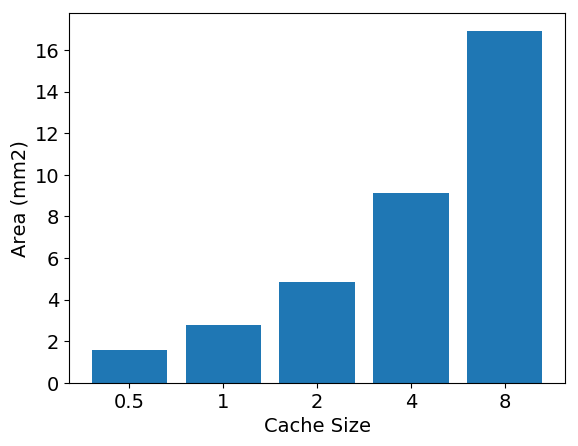
\includegraphics[width=\textwidth]{CacheArea.png}
        \caption{Cache Area vs. Cache Size}
    \end{subfigure}
    \begin{subfigure}[b]{0.5\textwidth}
        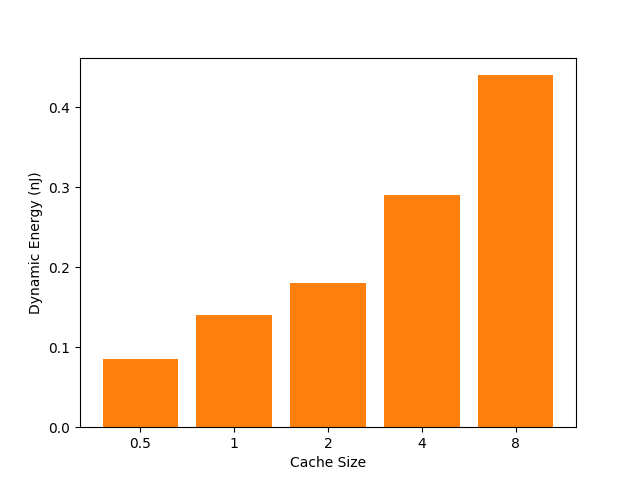
\includegraphics[width=\textwidth]{CacheEnergy.png}
        \caption{Dynamic Area vs. Cache Size}
    \end{subfigure}
    \begin{subfigure}[b]{0.5\textwidth}
        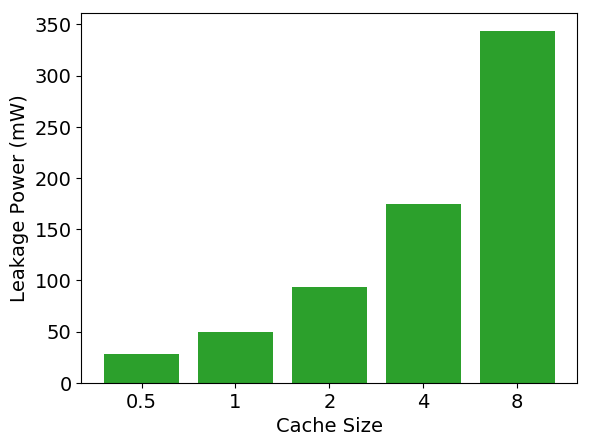
\includegraphics[width=\textwidth]{CachePower.png}
        \caption{Leakage Power vs. Cache Size}
    \end{subfigure}
    \begin{subfigure}[b]{0.5\textwidth}
        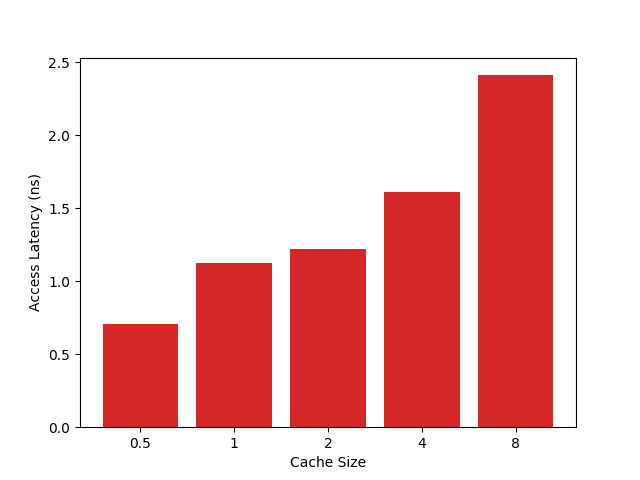
\includegraphics[width=\textwidth]{CacheLatency.png}
        \caption{Access Latency vs. Cache Size}
    \end{subfigure}
    \caption[Tradeoffs of Cache Size]{Showing how different cache traits are affected by cache size.}
    \label{fig:CacheSize}
\end{figure}
A different approach that has gained more popularity recently is to use compression to better utilize the existing cache space instead of increasing cache sizes. Cache compression allows caches to store more than their physical sizes, essentially acting like bigger size caches. However, they also impose more constraints on the compression and decompression design, requiring it to be very fast to not affect the cache performance. Previous proposals discussed and exploited data similarities and redundancies on different granularities. Some studies have found that applications can exhibit a lot of zero cache lines, some proposals were completely focused on zero compression~\cite{zca} while others treated zero lines as a special case in their compression schemes~\cite{fpc, hycomp, dedup}. Other proposals took advantage of the existence of data similarities of different granularities across caches. Such approaches used dictionaries for intra-line granularity~\cite{cpack, dish} or used deduplications~\cite{dedup} to take advantage of inter-line granularity similarities. Some studies opted to do data compression to decrease the data size on a line or smaller granularity rather than exploit existing cache wide data patterns~\cite{bdi, sc2, hycomp}.\par
The previously mentioned compression approaches do improve the utilization of cache space. However, each of those approaches focused on only one of two granularities to do compression. This first granularity was intra-line, only concerned about compressing data inside one data line to make the data line smaller and thus fit more than one data line in one physical cache line. The second granularity was inter-line, focusing only on reducing the total number of cache lines by getting rid of zero lines or deduplicating similar lines.\par
Some of today's applications can benefit from only one of those while others can benefit from both of them. For example, the dedup~\cite{parsec} benchmark is only inter-line compressible through deduplication~\cite{dedup}, the inversek2j~\cite{axbench} benchmark is only intra-line compressible, while the bwaves~\cite{spec} benchmark is compressible using both. It is obvious that only using one of the compressions on only one of the granularities is always missing some opportunity. Combining inter and intra-line compressions is the only way to gain the maximum possible compression and the highest benefits. But doing so also means that the cache organization is more complex, requires redesigning replacement policies, and more overhead. To our knowledge, no previous proposals have considered a compressed cache doing inter and intra-line compression at the same time.\par
In this work we pick two cache compression algorithms to cover inter and intra-line. We discuss their cache structures, compression, replacement policies, and their effect on different applications in Chapter~\ref{ch:BackgroundMotiv}. Then we describe how to combine both compression schemes in a cache in Chapter~\ref{ch:Design}. In the same chapter we also describe the effects and constraints it imposes on cache organization and replacement policies, and establish a roofline model for evaluation. In Chapter~\ref{ch:Results} we show the results of our implementation against the two selected algorithms, we also show how the performance of our cache varies with multiple design choices and parameters. Chapter~\ref{ch:Related Work} describes related cache compression techniques other than the two we picked.

%    2. Main body
% Generally recommended to put each chapter into a separate file
%% The following is a directive for TeXShop to indicate the main file
%%!TEX root = diss.tex

\chapter{Background and Motivation}
\label{ch:BackgroundMotiv}

%%%%%%%%%%%%%%%%%%%%%%%%%%%%%%%%%%%%%%%%%%%%%%%%%%%%%%%%%%%%%%%%%%%%%%
%%
%% Opportunity
%%
%%%%%%%%%%%%%%%%%%%%%%%%%%%%%%%%%%%%%%%%%%%%%%%%%%%%%%%%%%%%%%%%%%%%%%

\section{Opportunity}
\label{sec:Opportunity}
\begin{figure}
    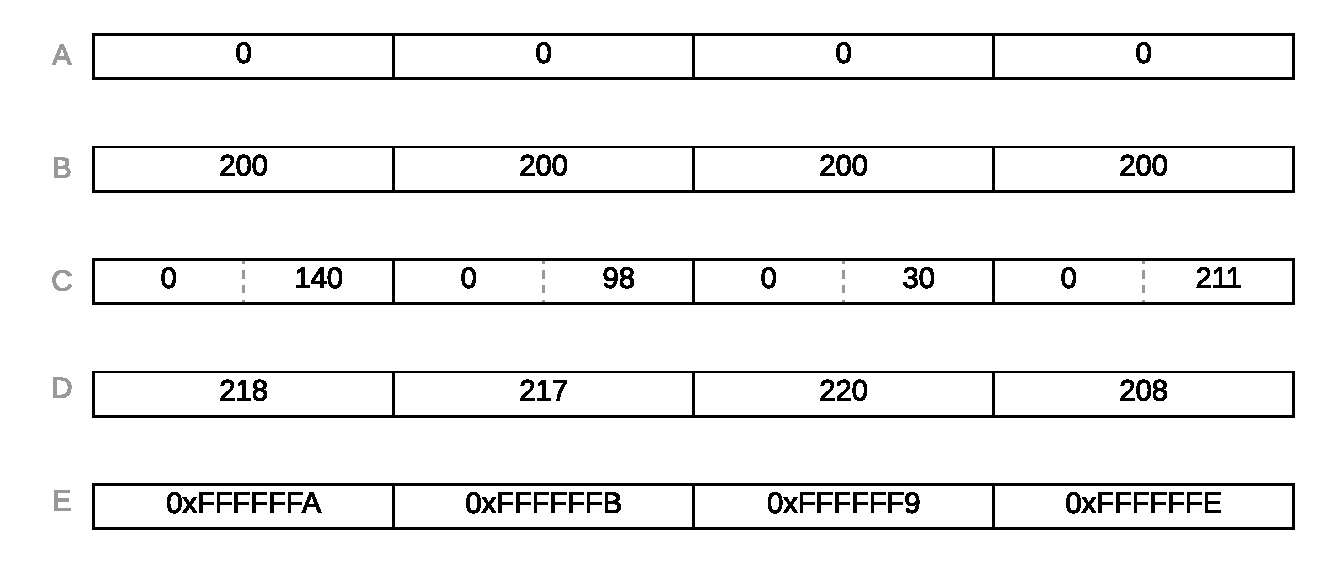
\includegraphics[width=\textwidth]{Patterns.pdf}
    \caption[Patterns in cache lines]{Some of the patterns observed in cache lines.}
    \label{fig:Patterns}
\end{figure}
\begin{figure}
    \begin{subfigure}[t]{\textwidth}
        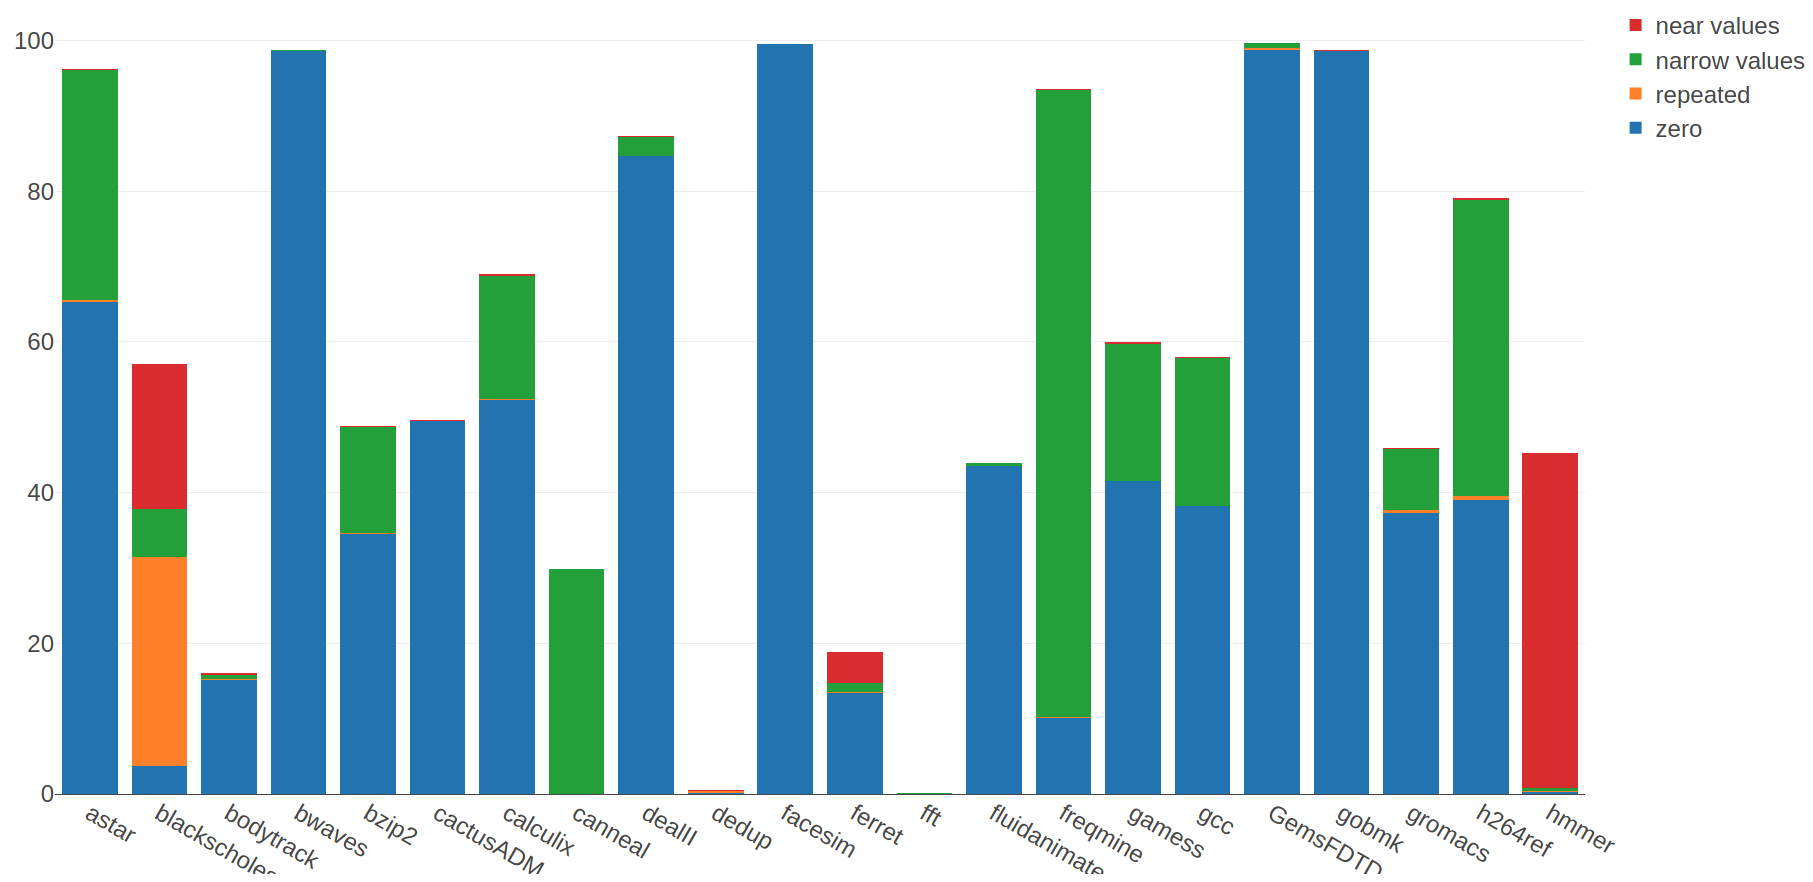
\includegraphics[width=\textwidth]{BDIPotential1.png}
    \end{subfigure}
    \begin{subfigure}[b]{\textwidth}
        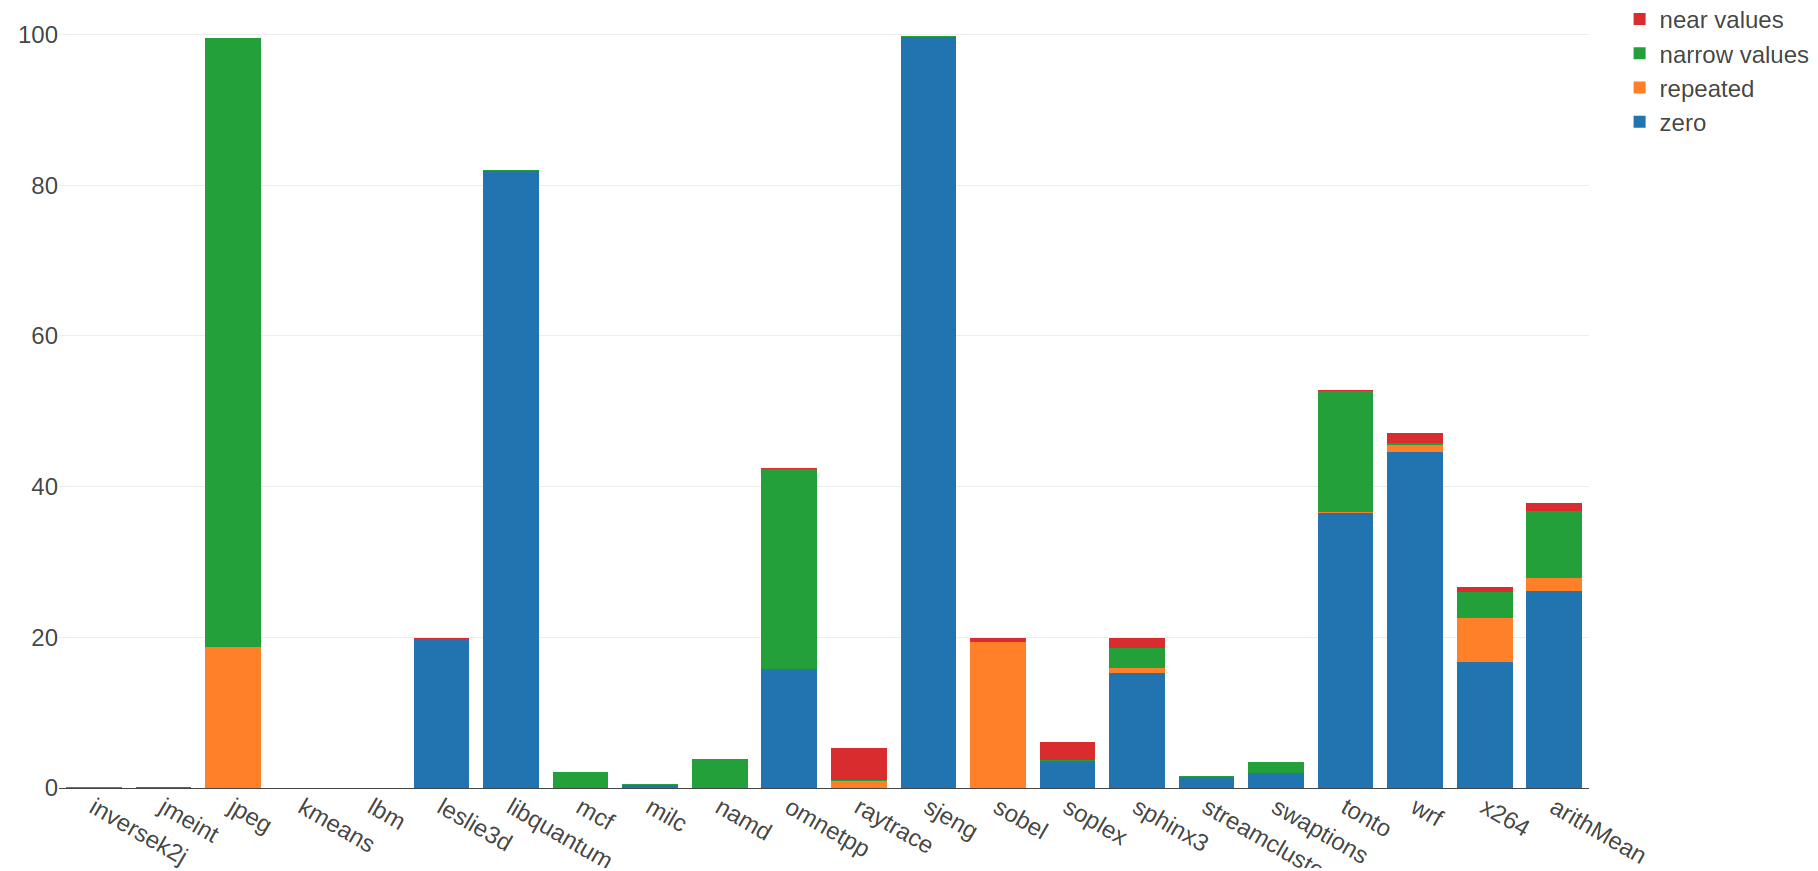
\includegraphics[width=\textwidth]{BDIPotential2.png}
    \end{subfigure}
    \caption[Intra-line Patterns]{The figure shows the percentage of cache lines that have one of the following patterns: zero, repeated values, narrow values, or near values. Recreated from \protect\cite{bdi}}
    \label{fig:BDIPotential}
\end{figure}
\begin{figure}
    \begin{subfigure}[t]{\textwidth}
        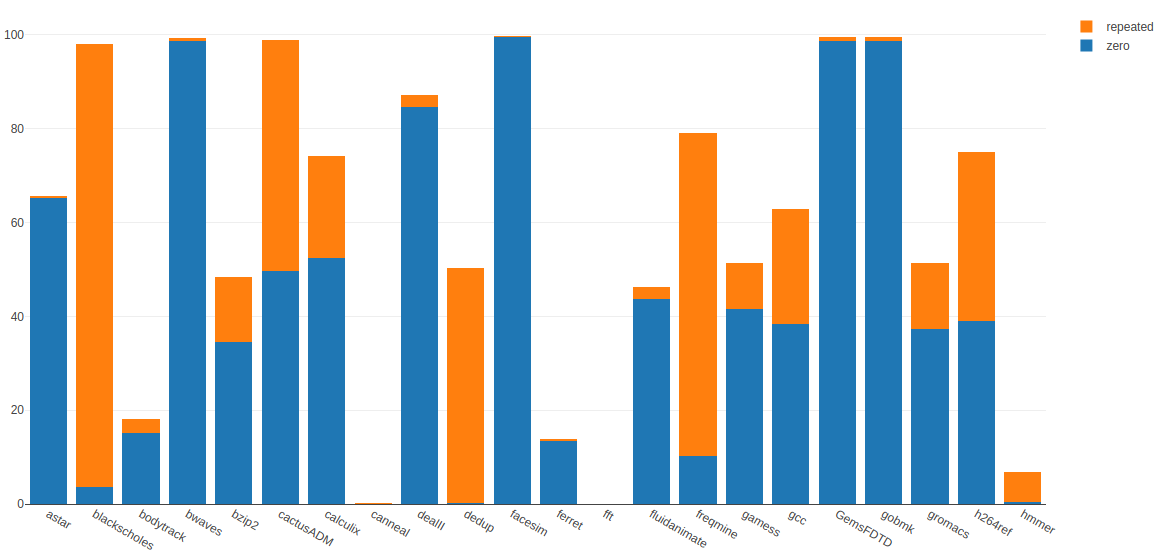
\includegraphics[width=\textwidth]{DedupPotential1.png}
    \end{subfigure}
    \begin{subfigure}[b]{\textwidth}
        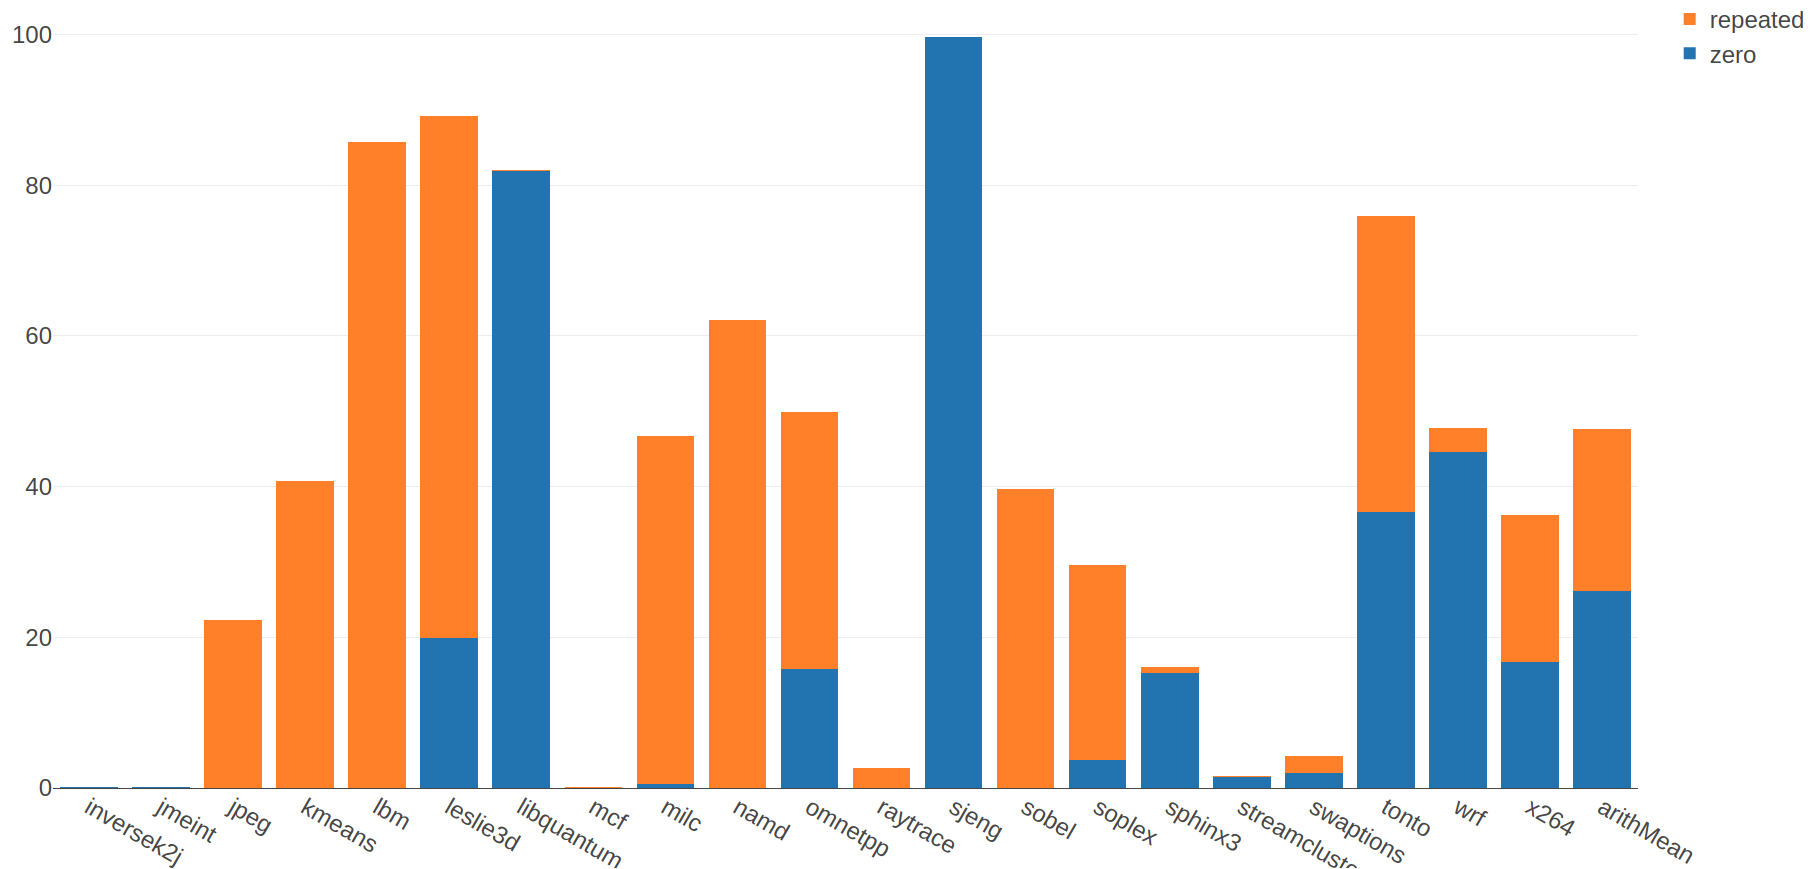
\includegraphics[width=\textwidth]{DedupPotential2.png}
    \end{subfigure}
    \caption[Inter-line Patterns]{The figure shows the percentage of similar cache lines in a cache, those present an opportunity for deduplication. Recreated from \protect\cite{dedup}}
    \label{fig:DedupPotential}
\end{figure}
Caches have been observed to have a great degree of redundancy when used with real world applications, those patterns can be observed on different granularities. We consider the patterns found on a cache line granularity, and on granularities smaller than a cache line. Some of those patterns are shown in Figure \ref{fig:Patterns} and are described as follows:
\begin{enumerate}
    \item \textbf{intra-line granularity:}
    \begin{enumerate}
        \item \textbf{Zeros:} A lot of cache data lines are fully zeros\cite{balakrishnan2003exploiting, ekman2005robust, yang2000frequent}. This is a very common case because zeros are usually used to initialize data structures. They're also very common in applications that deal with sparse matrices. Shown in part A of the figure.
        \item \textbf{Repeated Values:} Where a full cache line can contain the same value\cite{sazeides1997predictability, alameldeen2004adaptive}. This can be observed in applications that initialize large arrays to the same initial value, or in multimedia applications where adjacent pixels could hold the same colours. Shown in part B of the figure.
        \item \textbf{Narrow Values:} Programmers typically code for the worst case and thus have to pick larger data types while the majority of the values can fit in smaller narrower data types\cite{alameldeen2004adaptive, islam2010characterization, wilson1999case}. An example is a cache line of 32 bit integers where all the integer values are less than 256. A similar case is shown in part C of the figure.
        \item \textbf{Near Values:} Lines that contain values that are somewhat similar but not exactly, those are values that have high entropy in their lower bits but have the same higher bits. An example would be a list of pointers that are in the same memory regions, or pixels of an image that have almost similar colours\cite{wilson1999case, sun2008dhtc}. Part D and E of the figure show examples of this case.
    \end{enumerate}
    \item \textbf{inter-line granularity:}
    \begin{enumerate}
        \item \textbf{Zero lines:} Similar to the first pattern in the previous point, this case is about data lines being fully zeros. The only difference here is that we consider different zero lines instead of one line being fully zeroed.
        \item \textbf{Repeated lines:} Multiple cache lines can be exactly the same. This can happen in scientific benchmarks that have symmetry\cite{dedup}. For example the benchmark bwaves\cite{spec} simulates a spherical blast wave around an origin point, which involves perfect similarities.
    \end{enumerate}
\end{enumerate}
Figures \ref{fig:BDIPotential} and \ref{fig:DedupPotential} show the percentage of cache lines where those inter-line and intra-line patterns occur. A modified version of the zsim\cite{zsim} simulator have been used to dump snapshots of the L3 cache every 100,000 L3 accesses, with a maximum of 10 dumps per benchmark. The figures were created by statically analyzing the dumps for patterns.

%%%%%%%%%%%%%%%%%%%%%%%%%%%%%%%%%%%%%%%%%%%%%%%%%%%%%%%%%%%%%%%%%%%%%%
%%
%% BDI Cache
%%
%%%%%%%%%%%%%%%%%%%%%%%%%%%%%%%%%%%%%%%%%%%%%%%%%%%%%%%%%%%%%%%%%%%%%%

\section{Intra-line Compression}
\label{sec:BDI}
The BDI cache introduced in \cite{bdi} is a cache that takes advantage of similarities within data lines to compress those lines into smaller sizes. In the following section we discuss the BDI cache, it's compression, structure, and operation.
\subsection{Compression}
\label{Compression}
\subsubsection{Base Delta Compression}
In the previously mentioned patterns, the data in a cache line granularity have a low dynamic range, the difference between values in one cache line can be represented using fewer bytes than the original data type. A compression scheme was proposed to utilize this low dynamic range. It works by representing the data line using a base value, and an array of delta values. Since the delta values can be smaller in size than the original data elements, this allows for a lot of savings in the data line itself. If the delta size required to represent the delta is not smaller than the original size, the line is then not compressible and is left untouched.\par
Finding the right base is key to compress the data line optimally, and it happens in two steps:
\begin{itemize}
    \item \textbf{Finding the base size:} The right base size would affect the deltas and their sizes, and thus will affect the final compression size. Since caches have no knowledge of the data types stored in them, compression is not able to identify whether a specific data line is comprised of 16 bit integers or 32 bit floats and so the base size is not directly known. Choosing one base size statically would greatly reduce the opportunity for compression, so the authors opted to allow three different base sizes: 2, 4 and 8 bytes that can used simultaneously and the one that provides the best compression should be used.
    \item \textbf{Finding the base value:} Once a base size is chosen, the base value itself mush be found. Ideally, selecting the base value in a compressed line should be in the middle point between the minimum and the maximum values of a cache line. To avoid the hardware implementation complexity of finding the base, the authors opted to use the first value as base.
\end{itemize}
The allowed compression schemes and compressed sizes are shown in Figure \ref{fig:BaseDeltaCompression} and table \ref{tab:BDICompressionSizes}.
\begin{figure}
    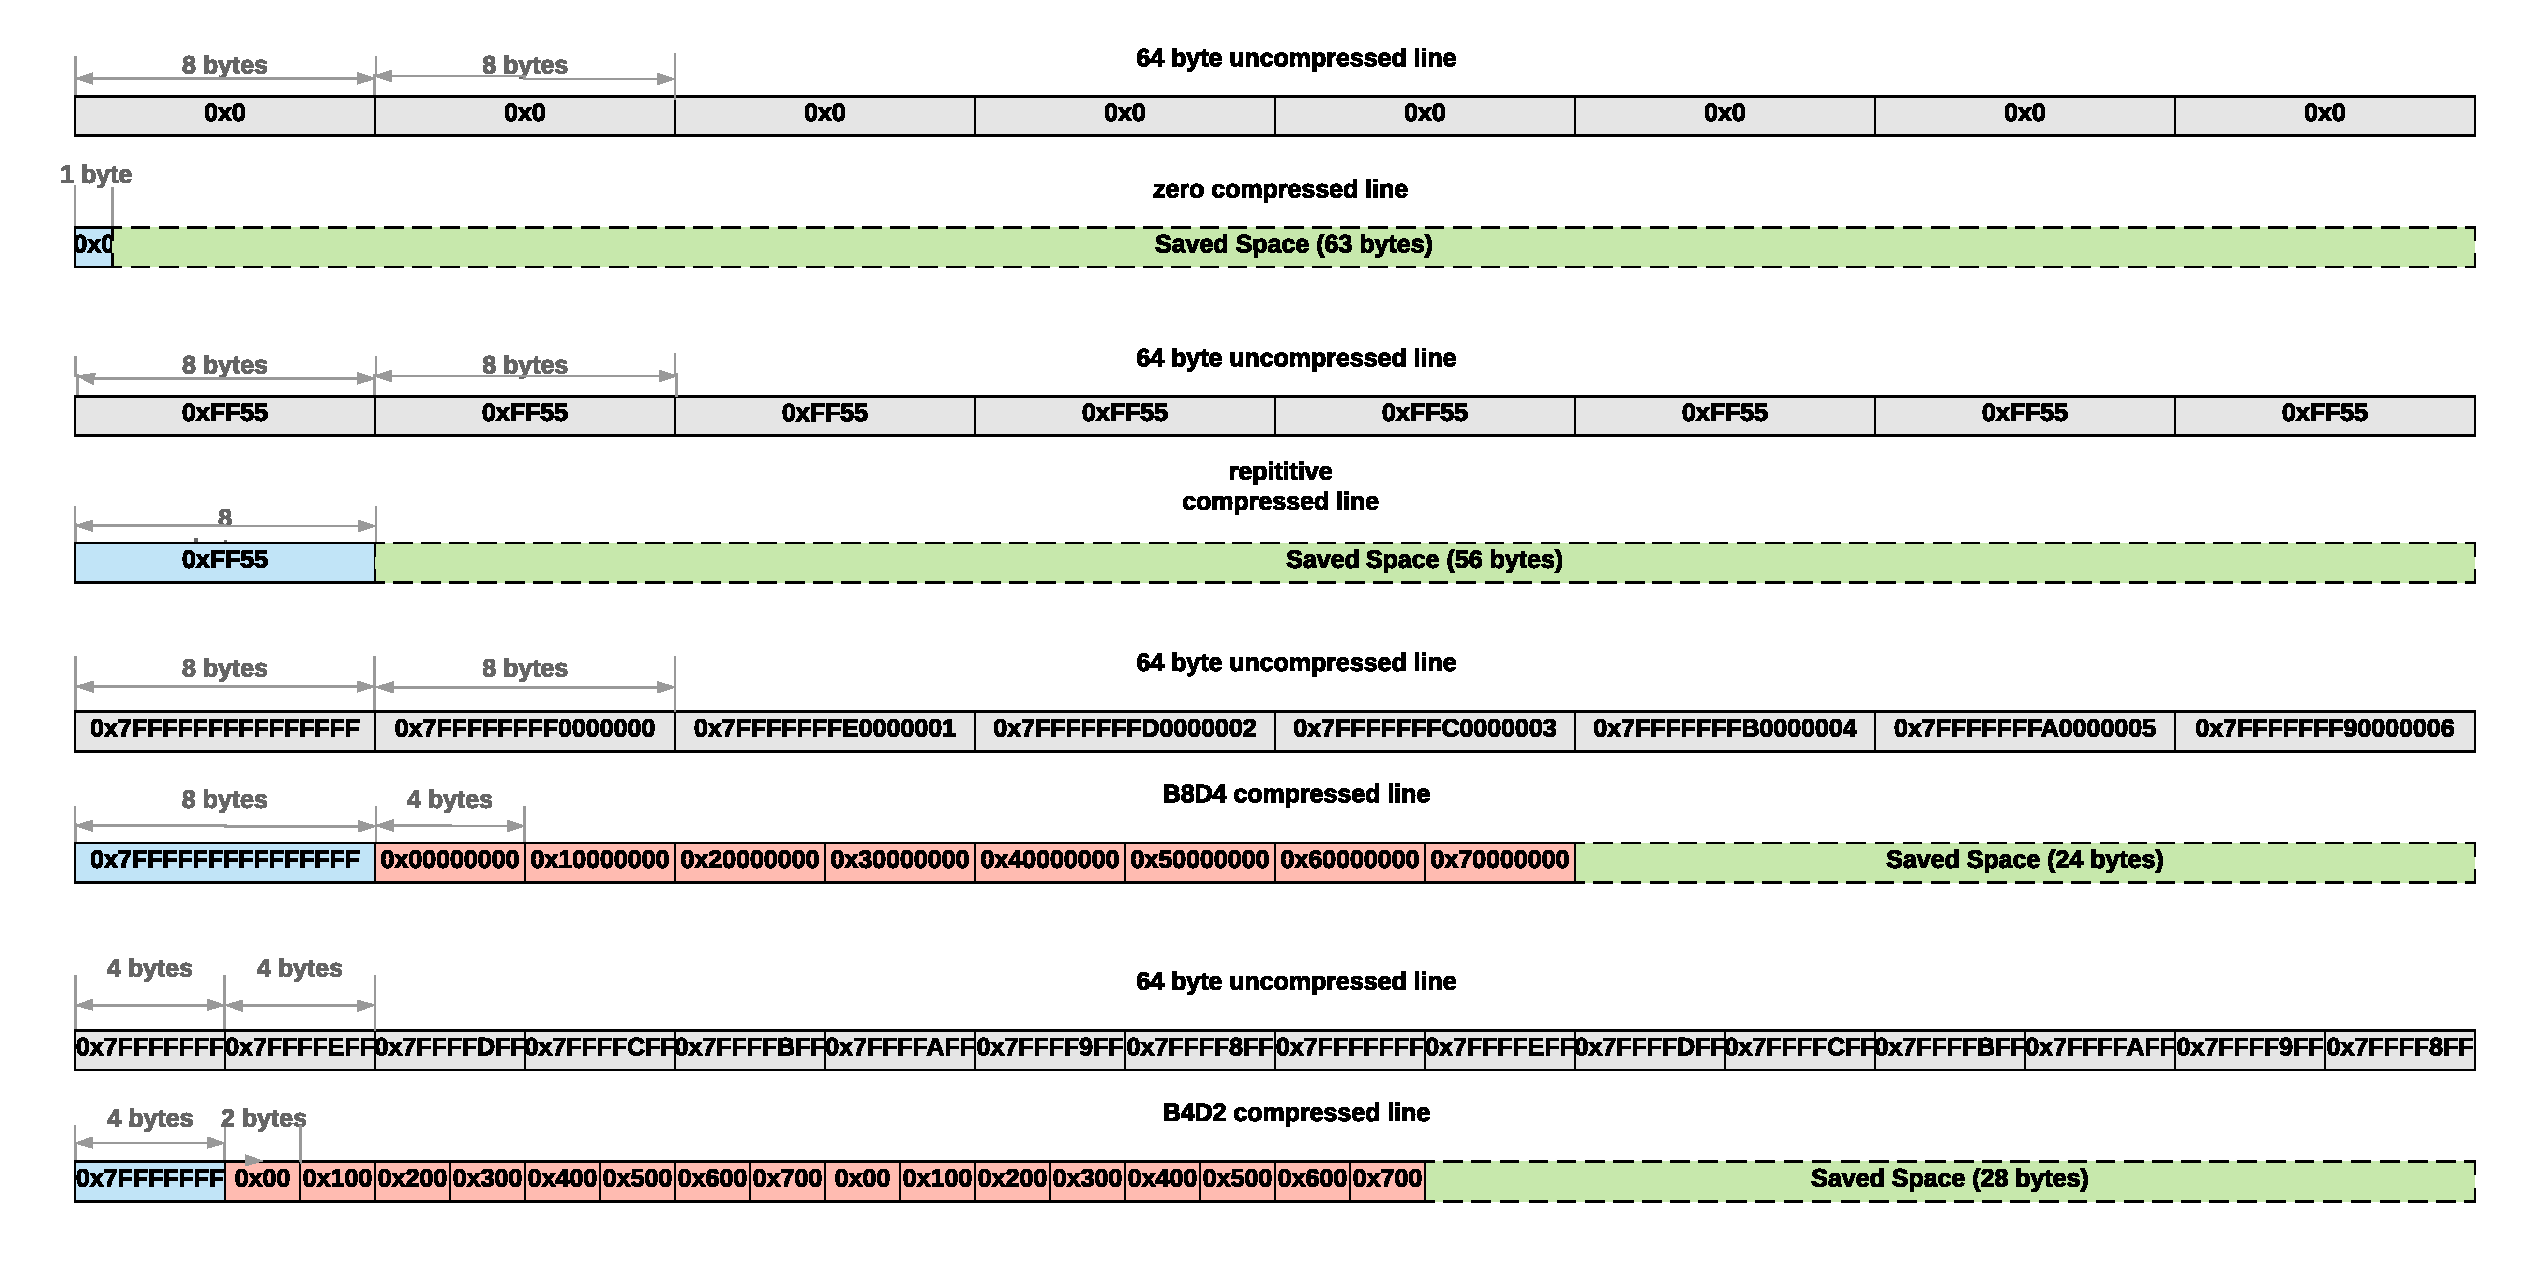
\includegraphics[width=\textwidth]{BaseDeltaCompression.pdf}
    \caption[Base Delta Compression Examples]{The figure shows examples of different cases of Base Delta compression.}
    \label{fig:BaseDeltaCompression}
\end{figure}
\subsubsection{Base Delta Immediate Compression}
Although one can gain a lot of compression from the base delta compression scheme, some patterns cannot be represented just by one base value. An example would be applications that use structs comprising of different data types. Because of this, allowing the base delta compression to use more than one base might help compress such lines. Based on experiments in \cite{bdi} it was clear that bases more than two do not provide much compression, so the authors selected two bases as their optimum number. To avoid the complexity of looking for a second base when compressing a data line, the authors opted to use the second base as an implicit zero. The intuition behind this is when structs are used in applications, they're likely to contain wide values with low dynamic range (e.g. Pointers) along with narrow values, the authors observe that using an implicit zero base captures most of the compression enabled by using an arbitrary second base.
\begin{table}[]
\centering
\caption[BDI Sizes]{The table shows BDI compression sizes, all sizes are in bytes. Original line size is 64 bytes.}
\label{tab:BDICompressionSizes}
\begin{tabular}{|c|c|c|c|c|}
\hline
\textbf{Name}         & \textbf{\begin{tabular}[c]{@{}c@{}}Base\\ Size\end{tabular}} & \textbf{\begin{tabular}[c]{@{}c@{}}Delta\\ Size\end{tabular}} & \textbf{\begin{tabular}[c]{@{}c@{}}Compression\\ Size\end{tabular}} & \textbf{\begin{tabular}[c]{@{}c@{}}Compression\\ Encoding\end{tabular}} \\ \hline
\textbf{Zero}         & 1                                                            & 0                                                             & 1                                                                   & 0000                                                                    \\ \hline
\textbf{Rep}          & 8                                                            & 0                                                             & 8                                                                   & 0001                                                                    \\ \hline
\textbf{B8D1}         & 8                                                            & 1                                                             & 16                                                                  & 0010                                                                    \\ \hline
\textbf{B8D2}         & 8                                                            & 2                                                             & 24                                                                  & 0011                                                                    \\ \hline
\textbf{B8D4}         & 8                                                            & 4                                                             & 40                                                                  & 0100                                                                    \\ \hline
\textbf{B4D1}         & 4                                                            & 1                                                             & 20                                                                  & 0101                                                                    \\ \hline
\textbf{B4D2}         & 4                                                            & 2                                                             & 36                                                                  & 0110                                                                    \\ \hline
\textbf{B2D1}         & 2                                                            & 1                                                             & 34                                                                  & 0111                                                                    \\ \hline
\textbf{Uncompressed} & N/A                                                          & N/A                                                           & 64                                                                  & 1111                                                                    \\ \hline
\end{tabular}
\end{table}
\subsubsection{Compression Hardware}
\label{sssec:BDICompressionHardware}
The compression hardware used for BDI consists of eight units that operate simultaneously in parallel, two for the zero and repetitive compression schemes and six units for the three different bases with their deltas. Each unit corresponds for one of the compression sizes described in Table \ref{tab:BDICompressionSizes}. Each unit outputs whether the line can be compressed in its scheme or not, and if it can be compressed it also outputs the compressed line. If multiple units can compress the line then the selection logic picks the one with the least compressed size.
A compression unit treats the line as elements of its corresponding base size. It picks the first element as the base and then subtracts all the elements from the it. If all the results can be represented in the required delta size then the line is compressed. Figure \ref{fig:BDIHardware} shows the compression hardware.
\begin{figure}
    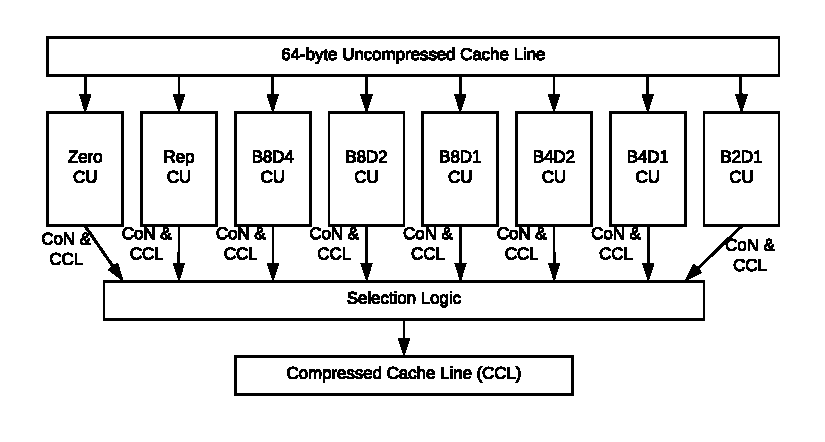
\includegraphics[width=\textwidth]{BDIHardware.pdf}
    \caption[BDI Compression Hardware]{The figure shows BDI compression hardware. CU: Compression Unit, CoN: Compressed or Not?, CCL: Compressed Cache Line. Recreated from \protect\cite{bdi}}
    \label{fig:BDIHardware}
\end{figure}

\subsection{Structure}
\label{ssec:BDIStructure}
\begin{figure}
    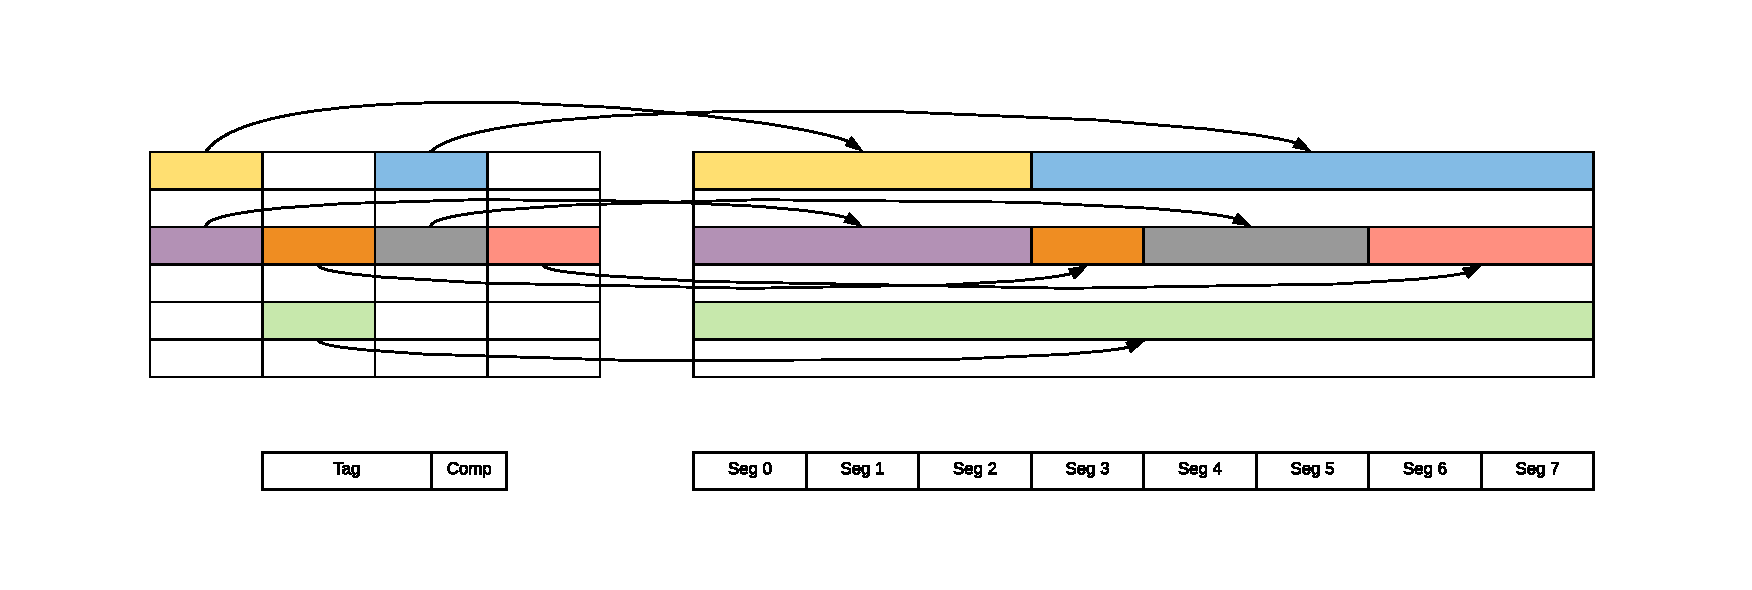
\includegraphics[width=\textwidth]{BDI.pdf}
    \caption[BDI Cache]{Conventional (up) vs BDI (down), showing one set of each. Tags doubled, Data size same but divided to segments.}
    \label{fig:BDI}
\end{figure}
The BDI cache builds upon the conventional cache design by adding some modifications to allow compression. Tag and data arrays are arranged in sets, and tag sets and data sets are coupled. The BDI cache structure is shown in Figure \ref{fig:BDI}
\subsubsection{Tag Array}
\label{sssec:BDITag}
Tag arrays in a BDI cache are no different than their counterparts in a conventional cache. The tags are arranged in sets and ways.\par
Along with its normal function, the tags also have two extra fields: A compression metadata field, and a Segment pointer. The compression metadata field describes the type of compression in the corresponding data line, it also contains a mask to distinguish which base is used for each delta. The segment pointer field is used to point to the first segment of the corresponding data line.\par
Other than the addition of compression metadata and segment pointer no other changes happen to the tag array. There are no constraint on its organization or replacement policy. However, because BDI potentially allows more data to be stored in the same cache size, more tags are needed to address this data. The tag array has to generally have more tags than data lines otherwise no benefits come out of compression.
\subsubsection{Data Array}
\label{sssec:BDIData}
Data lines in a BDI cache are logically divided into eight fixed size segments of eight bytes each (assuming a 64 byte cache line). A compressed data line can occupy any number of segments between one and eight. The data array does not save any metadata.\par
This general structure means the cache no longer has coupled tag and data \textit{lines} but it still maintains coupled data and tag \textit{sets}, i.e. A tag entry is no longer associated with a data entry in the corresponding location in the data array, but is associated with one of the segments in the corresponding set in the data array. The location of that segment depends on the compression encodings in the current selected tag set.

\subsection{Operations}
\label{ssec:BDIOperations}
\begin{figure}[h]
    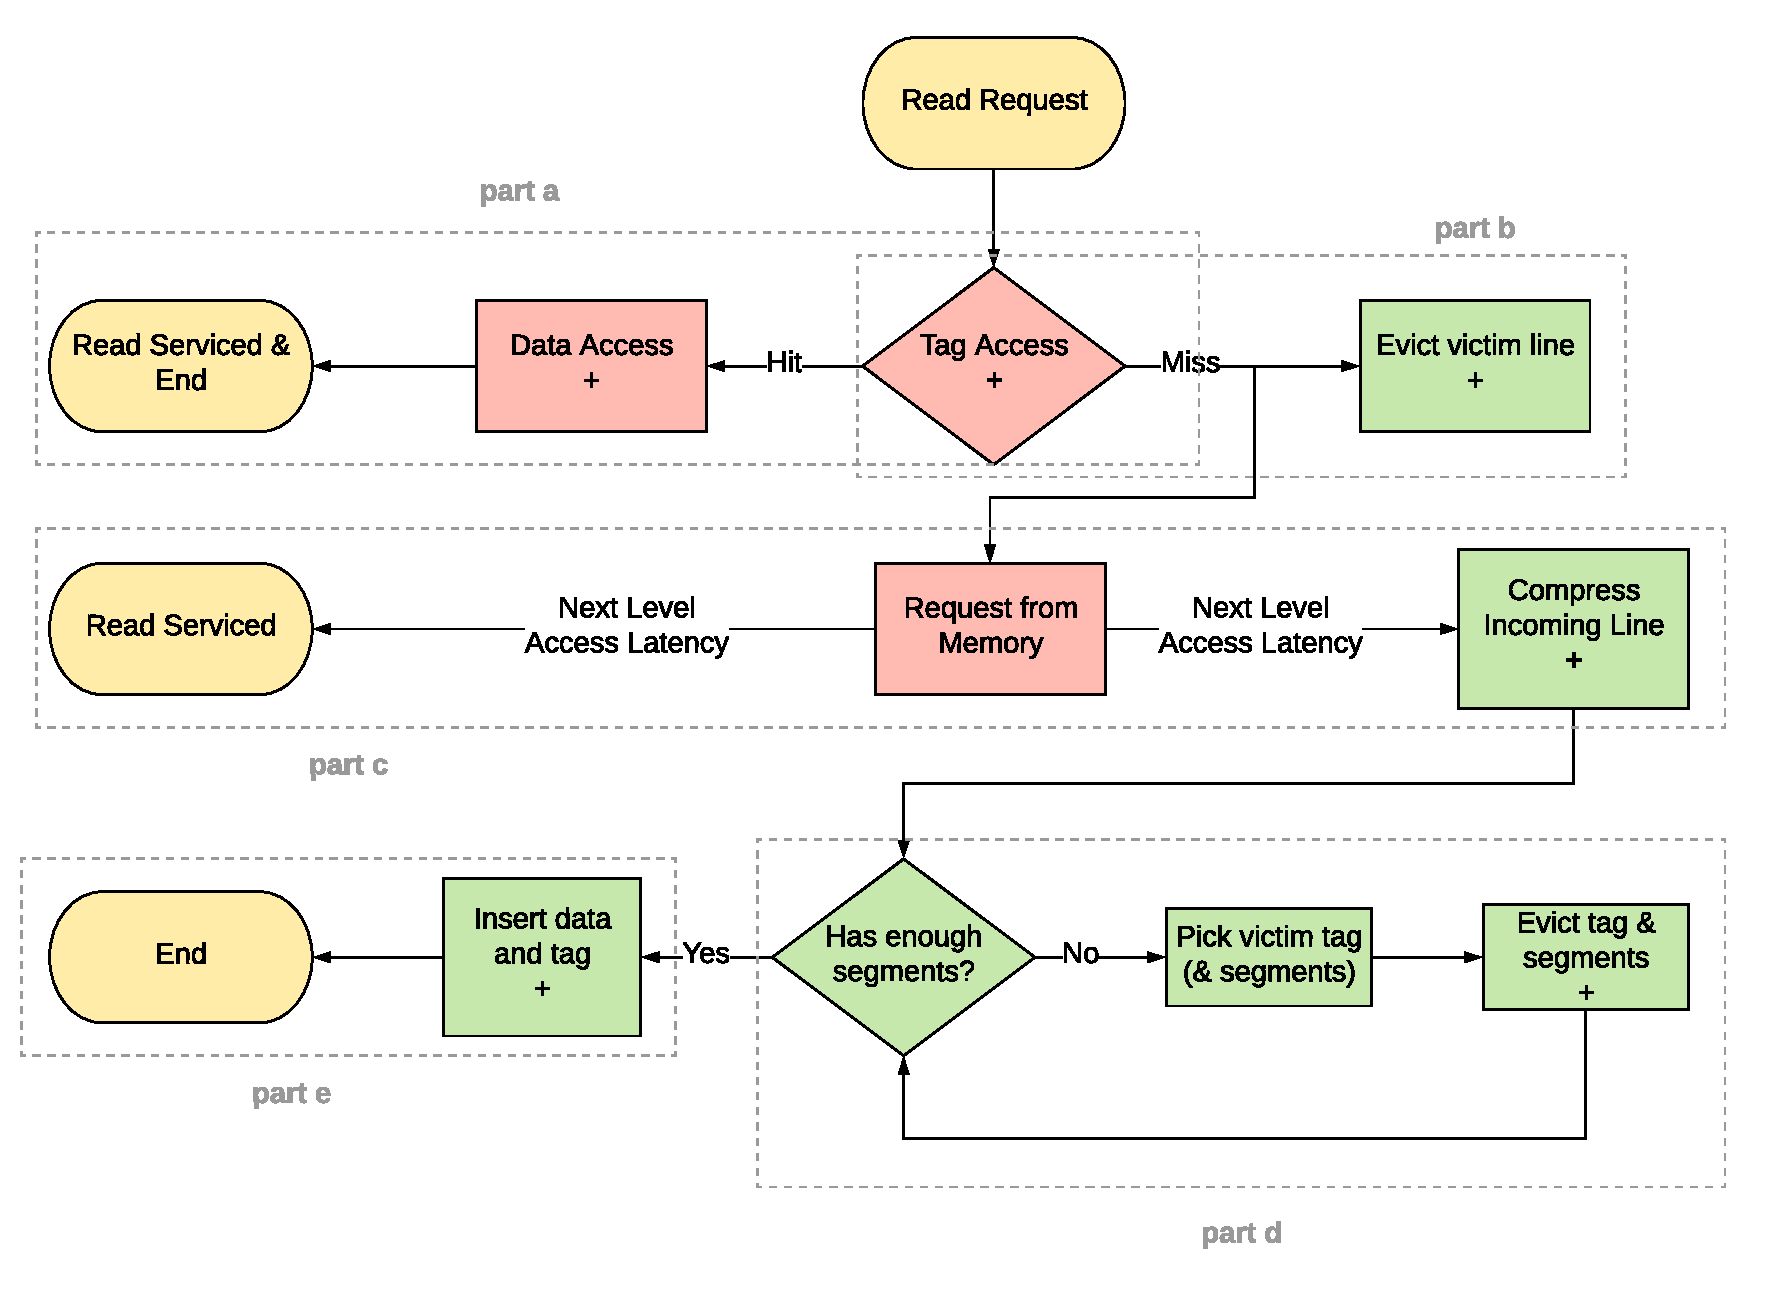
\includegraphics[width=\textwidth]{BDI_Read.pdf}
    \caption[BDI Read]{The flowchart shows the sequence of actions triggered by a read access to the BDI cache. Red blocks signify actions happening on the critical path, while green blocks mean actions happening off the critical path. Each + sign in any of the blocks signifies an extra latency for tag array access, data array access, or compression.}
    \label{fig:BDI_Read}
\end{figure}
\subsubsection{Cache Read}
A flowchart for the BDI cache read is shown in Figure \ref{fig:BDI_Read}. When the request first arrives the tag array is accessed. Part a in the figure shows the case when the tag access results in a hit, then the data line can be read, decompressed, and sent back to the requester right away. If the tag access is a miss, as shown in part b, the victim line is evicted. Then at the same time in parallel a request is sent to the next cache level (or main memory). Once the requested line comes back from the next level it can be used to service the requester right away, inserting the line itself into the cache happens after that and off the critical path, as shown in part c.\par
So far through the access everything is similar to a conventional cache, Only the insertion of the new line is going to be different. The insertion of the new line starts in part c in the figure. Once the requested line comes back from next level, and in parallel to serving the requester, the line is BDI compressed. Then before the line is actually written to the cache we must verify that there is enough space in the data set for it. If there's not enough segments we have to trigger extra evictions in the current set to free up more segments, those evictions happen according to the tag replacement policy. The size caused evictions are shown in part d, and the line can finally be inserted once enough segments are available as shown in part e.\par
To avoid segmentation, the authors assume compaction always happens in the data array before each insertion, this is in accordance with previous work.
\begin{figure}[h]
    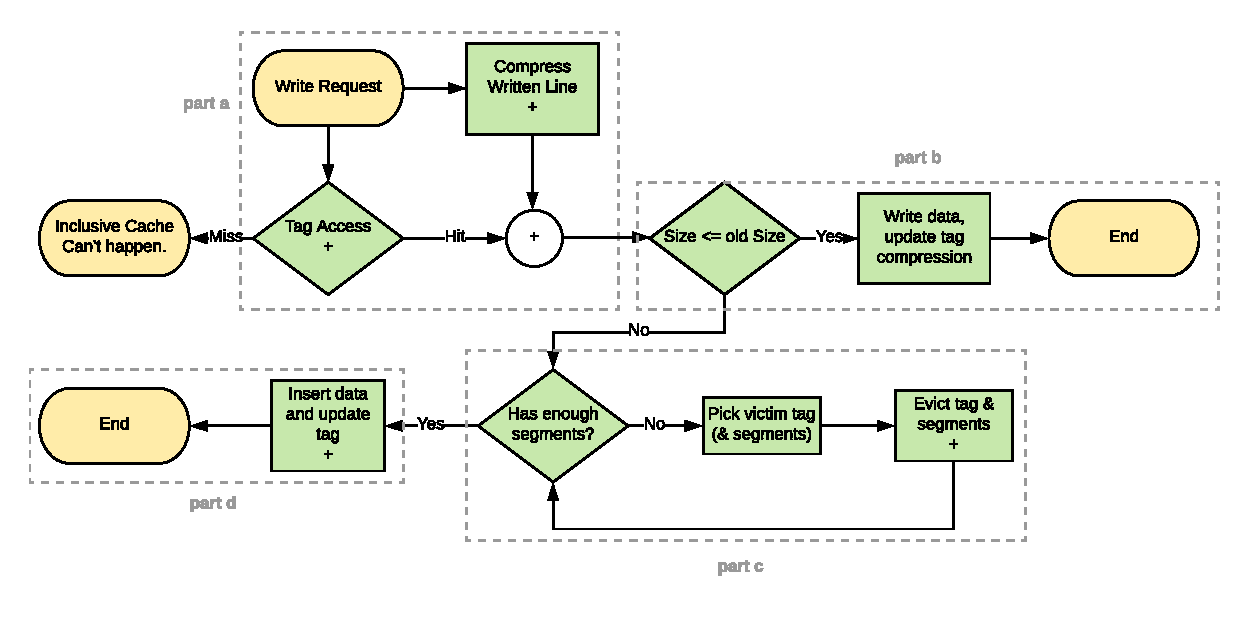
\includegraphics[width=\textwidth]{BDI_Write.pdf}
    \caption[BDI Write]{The flowchart shows the sequence of actions triggered by a write access to the BDI cache. All the blocks are shaded in green because any write request should be off the critical path of the processor regardless of its status in the cache (hit or miss). Each + sign in any of the blocks signifies an extra latency for tag array access, data array access, or compression.}
    \label{fig:BDI_Write}
\end{figure}
\subsubsection{Cache Write}
A flowchart of write access to a BDI cache is shown in Figure \ref{fig:BDI_Write}. Because we always use inclusive caches, if a line is in a lower level cache it must also be in it's parent. A cache miss on a write request thus can never happen and a tag array access on a write request will always yield a hit as shown in part a. In parallel to the tag access, the written data line can also be compressed. Once we know the size of the compressed line, we can check whether or not it fits in it's old size, if it's the same or requires a lower number of segments, shown in part b, it can be written right away and the compression metadata in the tag array must also be updated. If the new compressed size is bigger than the old size, insertion of the new written line will trigger size based evictions, the replacement policy will be consulted for tags and their segments to be evicted until enough space for the new data line is free, this is shown in part c. Once there's enough segments the line can finally be written and it's tag's metadata can be updated accordingly as shown in part d.
As mentioned previously, the authors assume compaction always happens in the data array before each insertion, this is in accordance with previous work.

%%%%%%%%%%%%%%%%%%%%%%%%%%%%%%%%%%%%%%%%%%%%%%%%%%%%%%%%%%%%%%%%%%%%%%
%%
%% Dedup Cache
%%
%%%%%%%%%%%%%%%%%%%%%%%%%%%%%%%%%%%%%%%%%%%%%%%%%%%%%%%%%%%%%%%%%%%%%%
\section{Inter-line Compression}
\label{sec:Dedup}
The Dedup cache was introduced in \cite{dedup}. The authors have found that in some applications, a lot of lines in the cache can be similar, as shown in Figure \ref{fig:DedupPotential}. Previous cache compression implementations have been proposed to take advantage of duplications, but only focused on special cases like zeros\cite{alameldeen2004adaptive, dusser2009zero}. The authors proposed and built a cache that takes full advantage of the line similarity by doing deduplication, getting rid of the redundant data copies and keeping only one. The structure and operation of such a cache is discussed in this section.
\subsection{Structure}
\label{ssec:DedupStructure}
\begin{figure}
    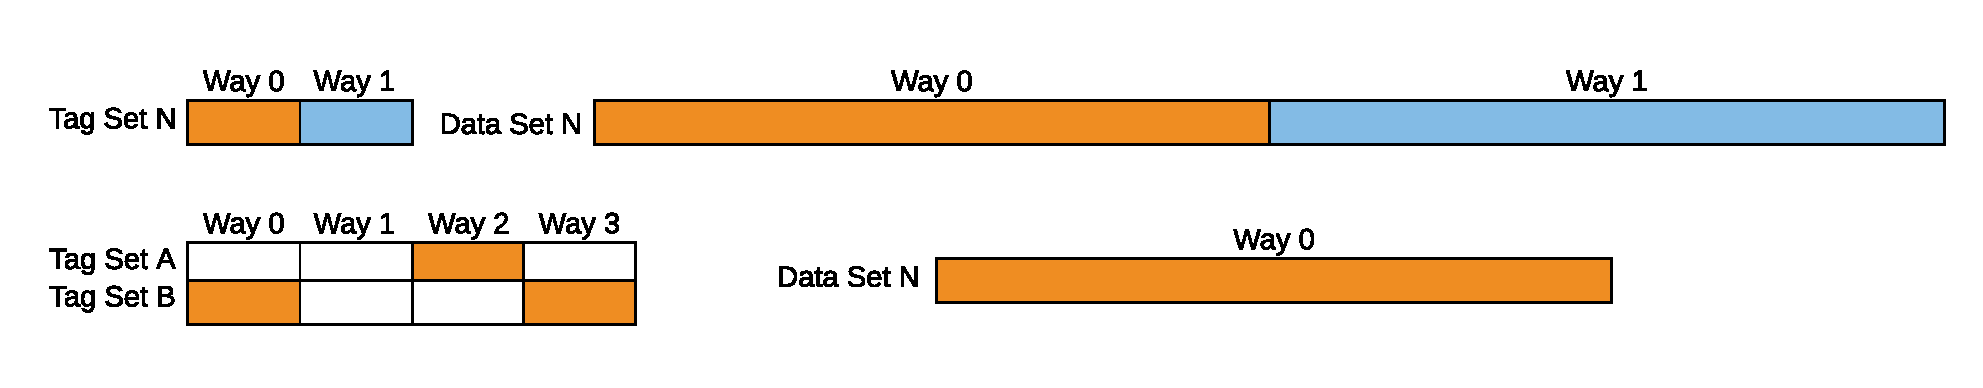
\includegraphics[width=\textwidth]{Dedup.pdf}
    \caption[Dedup Cache]{Conventional (up) vs Dedup (down), showing one set of tags and data from a conventional cache, but one set and related tags from a dedup cache. Tags doubled, Data size same but is now direct mapped.}
    \label{fig:Dedup}
\end{figure}
The Dedup cache introduces some major modifications on top of a conventional cache to support deduplication. The tag array is arranged as normal in sets and ways. The data array is no longer coupled with the tag array, instead it has to be explicitly accessed by pointers. So the data array has no constraints or requirements on its associativity, so it's simply left to be direct mapped. To take advantage of deduplications, the tag array must generally have more entries than the data array.\par
To facilitate finding and locating duplicate lines, a new structure is added to the cache, called the hash array. The hash array is a storage that saves hashes of data lines. Searching and comparing in the hash array makes it faster and cheaper than searching for duplicate lines directly in the data cache.

The Dedup cache structure is shown in Figure \ref{fig:BDI}

\subsubsection{Tag Array}
\label{sssec:DedupTag}
The Dedup tag array organization is no different than a tag array in a conventional cache, it's arranged in sets and ways.\par
To support deduplication, some other modifications to the tag array need to be made. Deduplication means more than one tag entry will share the same data entry. This poses two requirements on the Dedup cache: Tags must know which data line is the one they need, and if that data line gets evicted, all the tags that use it must be evicted too.\par
based on the previous requirements, some additions to the tag array entries must be made. For the tags to be able to address their corresponding data lines, a pointer to the data line must be added to the tag entry. Similarly, to facilitate eviction of all the tags connected to a data line when the line is evicted, those tags are organized in a linked list, so each tag entry has two previous and next pointers that point to the two tags before and after it in a linked list. Those pointers need to be big enough to only point to tag sets, since reading a tag requires reading the whole set, the required tag from that set can be resolved by comparing it's data pointer.\par
Other than the addition of the previous/next and data pointers, there are no other changes to the tag array, only that tags need to have more entries than data to take advantage of deduplication.
\subsubsection{Data Array}
\label{sssec:DedupData}
The data array in a Dedup cache is decoupled from the tag array, and thus it's not required to have the same associativity as the tag array. In fact, this means the data array is not required to have any associativity at all, it can be directly mapped.\par
To facilitate the eviction of the tags associated with the data line in case it gets evicted, the data lines have an extra metadata field, a tag pointer. This tag pointer is used to point to the first tag in the linked list associated with the data line, in case the data line is evicted the linked list is walked and all the tags in it are evicted.\par
The data line also includes an extra counter, this counter is used to track how many tags use this data line, this is useful to decide which data lines to evict.
\subsubsection{Hash Array}
\label{sssec:DedupHash}
The hash array in a Dedup cache is used to store hashes of some of the data lines, providing a way to facilitate finding similar lines and deduplicating them. The hash array is a simple set associative structure.\par
When a data line is hashed, its hash is split into two parts, one is used to index the hash array, while the other is saved in the hash array itself. This process is similar to how memory addresses access the tag array, where part of the address is used to index the array while the other part is saved in the array itself.\par
Along with each hash saved in the hash array, there's also a pointer to a data line that meets this hash, similar to the data pointers in tag arrays.\par
The hashes are computed through an XOR tree, based on experiments done in \cite{dedup}. The number of hash entries in the array is small. The authors in \cite{dedup} show that a small number of hash entries is enough to keep collisions less that 1\%.

\subsection{Replacement Policies}
\label{ssec:DedupRepl}
While the tag array in a Dedup cache maintains it's normal replacement policies, the data and hash array may have to be treated differently, since they're decoupled from the tag array.
\subsubsection{Data Array}
\label{sssec:DedupDataRepl}
The data array replacement policy can be split into two parts, the first part is uses a list to keep track of all free lines in the data array, this list is always consulted first for a free line to insert into. If the free list is empty, indicating that there are no free lines in the data array, the second part of the replacement policy is then used.\par
If no free lines are available, a random data line is selected, if that line is distinct (not deduplicated, has one tag), it's evicted and used for insertions, otherwise another random line is selected. This process is repeated up to four times, if after those four times no distinct line has been found, the line with the lowest deduplications is evicted and used for insertion.
\subsubsection{Hash Array}
\label{sssec:DedupHashRepl}
The hash array is indexed by a part of the hash, the selection of a victim hash set is thus dependant on the hash that needs to be inserted. Once that set is selected, a hash entry is then selected based on the number of deduplication on the data line it point to, if this data line is not deduplicated then this hash can be used and overwritten, otherwise it's not touched. The rationale behind this is to keep hashes pointing to deduplciated lines from getting evicted and causing the cache to miss extra deduplication in favour of a newly incoming line that might not be useful for deduplication.\par

\subsection{Operations}
\label{ssec:DedupOperations}
\begin{figure}[h]
    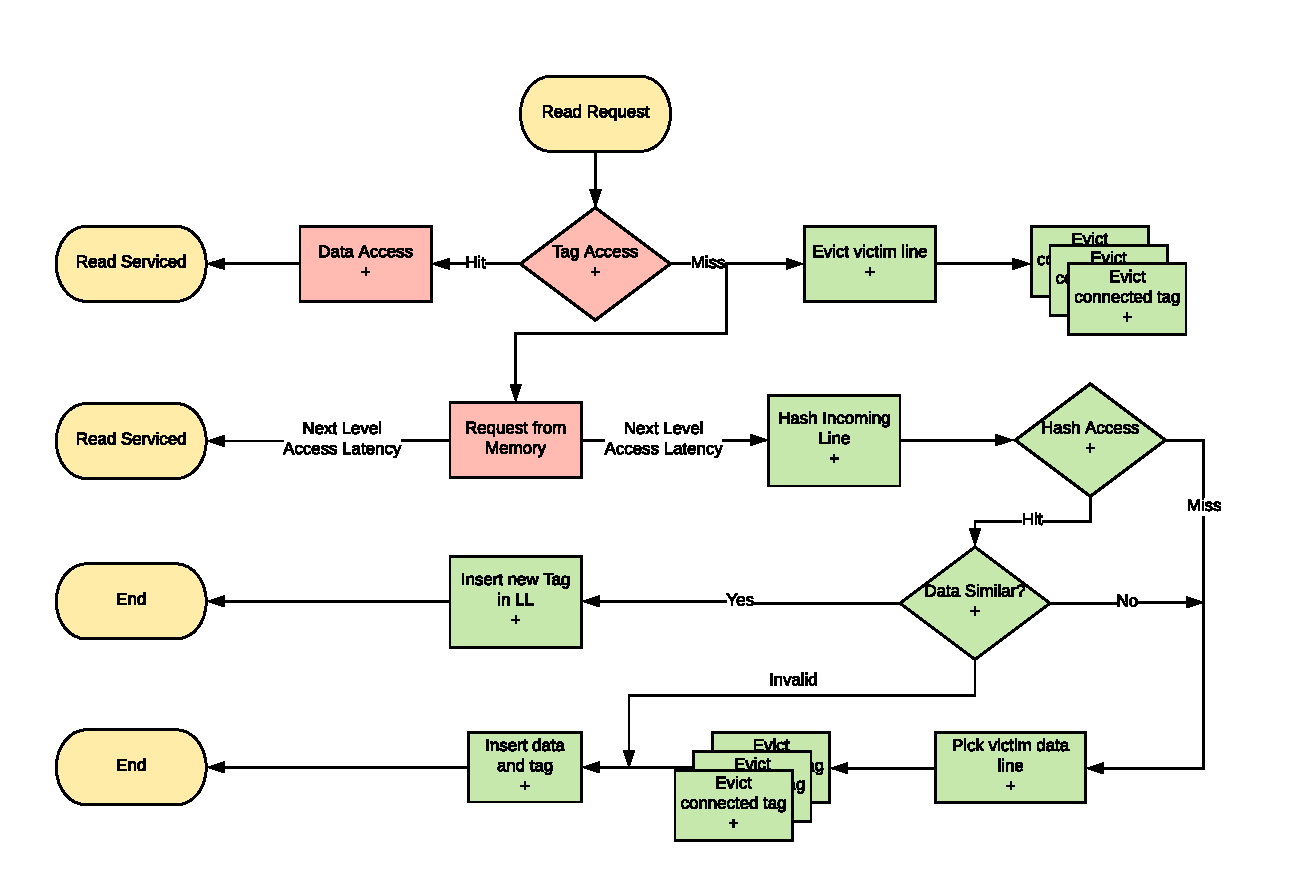
\includegraphics[width=\textwidth]{Dedup_Read.pdf}
    \caption[Dedup Read]{The flowchart shows the sequence of actions triggered by a read access to the Dedup cache. Red blocks signify actions happening on the critical path, while green blocks mean actions happening off the critical path. Each + sign in any of the blocks signifies an extra latency for tag array access, data array access, or compression.}
    \label{fig:Dedup_Read}
\end{figure}
\subsubsection{Cache Read}
A flowchart for the Dedup cache read is shown in Figure \ref{fig:Dedup_Read}. When the request first arrives the tag array is accessed. Part a in the figure shows the case when the tag access results in a hit, then the data line can be read and sent back to the requester right away. If the tag access is a miss, as shown in part b, a victim tag is evicted and it's linked list (if any) has to be updated (i.e. The pointers of the previous and next tags have to connect to each other instead of the victim.). At the same time and in parallel a request is sent to the next cache level (or main memory). Once the requested line comes back from the next level it can be used to service the requester right away, as shown in part c. Inserting the line itself into the cache happens after that and off the critical path.\par
So far through the access everything is similar to a conventional cache, Only the insertion of the new line is going to be different. The insertion of the new line starts in part d in the figure. Once the requested line comes back from next level, and in parallel to serving the requester, the line is hashed and the hash is used to access the hash array.\par
If the hash access hits, then the incoming line must be compared to the line pointed to by the hash, to make sure there are not collisions. There are four outcomes of this scenario, shown in part d:
\begin{itemize}
    \item \textbf{Hash Miss:} No similar hash is found, either because similar lines do not exist in the data array, or because the hash array is not big enough to keep track of all data lines. In this case we use the data replacement policy to evict a victim data line. The new tag is inserted and the tag and data lines have to point to each other, the tag will not point to other tags and will not create a linked list because no deduplication is happening yet. A new hash entry will be selected based on the hash replacement policy and will point to the newly inserted data line.
    \item \textbf{Hash Hit, Line Similar:} In which case the received data line can be deduplicated. It will use the same data line and hash entry. Only the new tag needs to be inserted. It is inserted as the head of the linked list and points to the deduplicated data line. The data line's tag counter (deduplication counter) has to be incremented and it has to point to the new linked list head.
    \item \textbf{Hash Hit, Line Invalid:} Because hashes point to data lines, but data lines do not point to hashes, when a data line is evicted, it's associated hash might not, causing a situation like this to arise. In this case, we utilize the invalid line right away instead of consulting the data replacement policy. The tag entry is inserted, it has to point to the data line, but it doesn't point to any other tags because the data line is not deduplicated yet and shouldn't have a linked list associated with it. The data line in return also points to the tag entry, the hash entry is not changed because it already points to the space we used for the data line.
    \item \textbf{Hash Hit, Line Different:} This case happens only on a hash collision, when two different data lines can be hashed to the same value. Once a collision happens, it's treated like a hash miss with one modification: a new hash insertion is not needed. The same hash entry will be changed to point to the newly inserted data line in only if the line it was previously pointing to was not deduplicated (i.e. Its tag counter is 1). Otherwise it remains untouched.
\end{itemize}

\begin{figure}[h]
    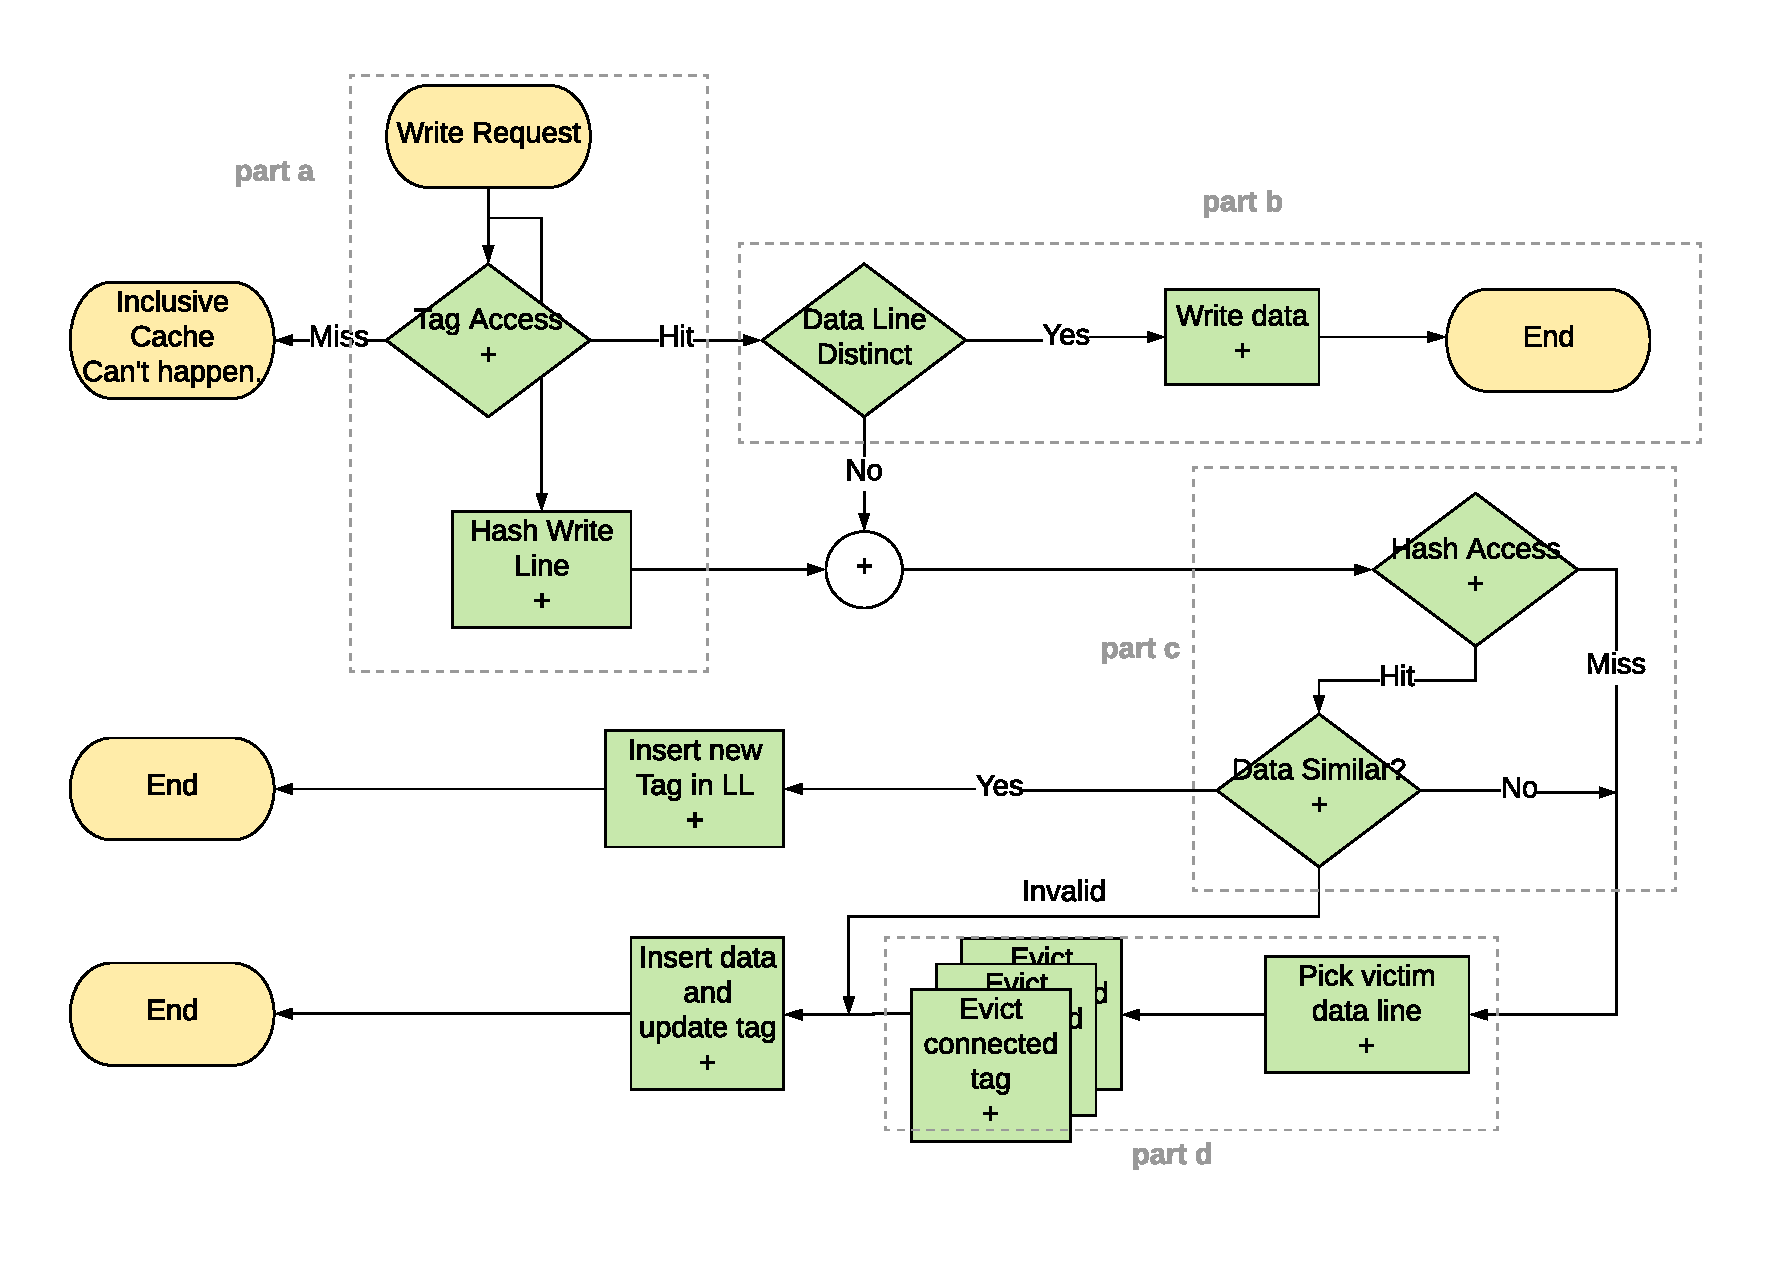
\includegraphics[width=\textwidth]{Dedup_Write.pdf}
    \caption[Dedup Write]{The flowchart shows the sequence of actions triggered by a write access to the Dedup cache. All the blocks are shaded in green because any write request should be off the critical path of the processor regardless of its status in the cache (hit or miss). Each + sign in any of the blocks signifies an extra latency for tag array access, data array access, or compression.}
    \label{fig:Dedup_Write}
\end{figure}
\subsubsection{Cache Write}
A flowchart of write access to a Dedup cache is shown in Figure \ref{fig:Dedup_Write}. Because we always use inclusive caches, if a line is in a lower level cache it must also be in it's parent. A cache miss on a write request thus can never happen and a tag array access on a write request will always yield a hit as shown in part a. In parallel to the tag access, the written data line can also be hashed.\par
Once the tag access is finished, we can find out whether the line was distinct or not. If the line is distinct and had no other tags associated with it, then it can be written to right away as shown in part b. If the line is deduplicated, then a write to the line can change it and cause that tag to lose similarity. The insertion of the written data line then can be handled similarly to a miss. It has to access the hash array and look for similar lines, this has one of the four outcomes described above as shown in parts c and d.

\section{Motivation}
\label{sec:Motivation}
Deduplication and base delta immediate compression work on two different domains, one is inter-line and works on a cache line granularity while the other works intra-line with a granularity of two, four, or eight bytes. This means that they can both be combined to deduplicate similar lines and compress each of those lines at the same time.
We look at four different benchmarks with different cache patterns and behaviours. One benchmark is very compressible by BDI, the second is compressible using deduplication, the third and fourth are completely incompressible and compressible by both, respectively. We analyze how these benchmarks respond to each type of compression and how a combination of both compression techniques can improve on them.\par
The four benchmarks are:
\begin{figure}
    \begin{subfigure}{\textwidth}
        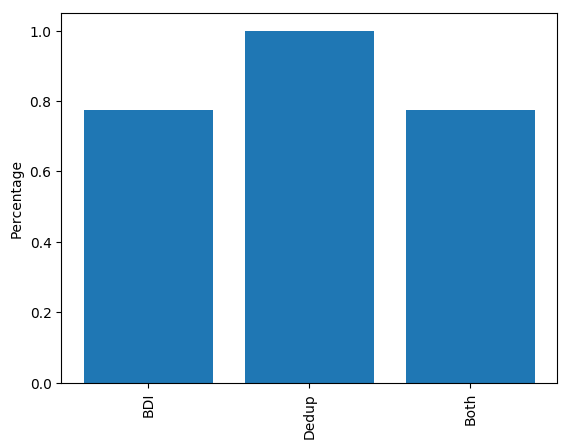
\includegraphics[width=\textwidth]{canneal.png}
        \caption{canneal}
        \label{fig:canneal}
    \end{subfigure}
    \begin{subfigure}{\textwidth}
        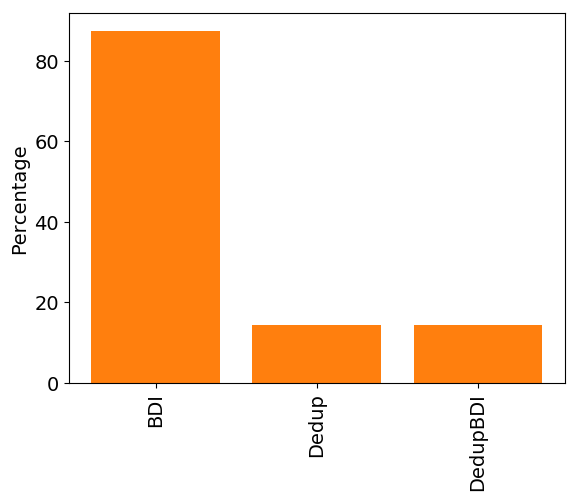
\includegraphics[width=\textwidth]{lbm.png}
        \caption{lbm}
        \label{fig:lbm}
    \end{subfigure}
    \begin{subfigure}{\textwidth}
        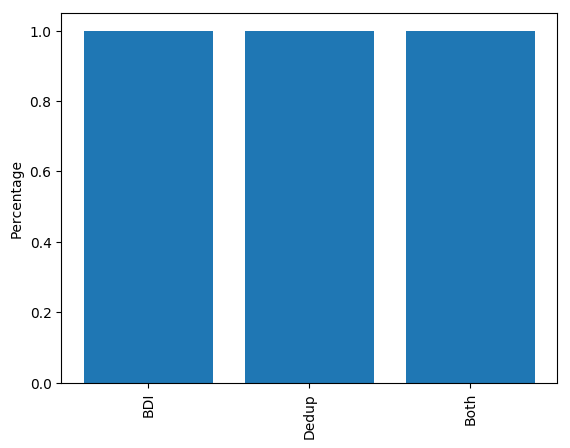
\includegraphics[width=\textwidth]{jmeint.png}
        \caption{jmeint}
        \label{fig:jmeint}
    \end{subfigure}
    \begin{subfigure}{\textwidth}
        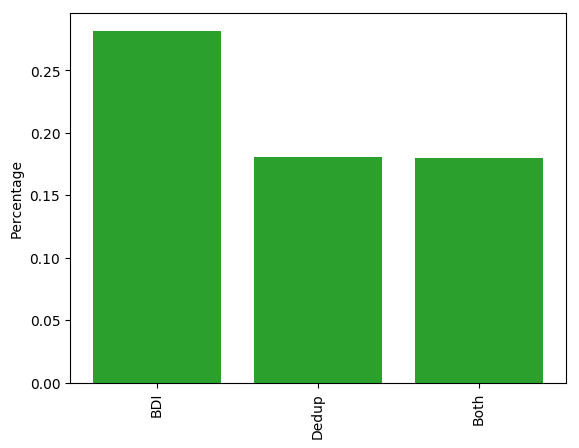
\includegraphics[width=\textwidth]{libquantum.png}
        \caption{libquantum}
        \label{fig:libquantum}
    \end{subfigure}
    \caption[Compression in benchmarks]{The figure shows the percentage of compressed data compared to original cache sizes.}
\end{figure}
\begin{itemize}
    \item \textbf{canneal:} The canneal benchmark\cite{parsec} is a cache-aware implementation of a simulated annealing algorithm used for routing in chip designs. canneal is BDI sensitive but doesn't have enough potential to benifit from deudplication. Figure \ref{fig:inversek2j} shows the Dedup, BDI, and Dedup+BDI compressed data size of canneal cache dumps as a percentage of the original size.
    \item \textbf{lbm:} The lbm benchmark\cite{spec} implements the "Lattice Boltzman Method" to simulate incompressible fluids in 3D. The output from lbm benchmark is values representing 3d velocity vectors for each cell in the simulation. Because of this, lbm is deduplication sensitive. Figure \ref{fig:lbm} shows the Dedup, BDI, and Dedup+BDI compressed data size of lbm cache dumps as a percentage of the original size.
    \item \textbf{jmeint:} The jmeint benchmark\cite{axbench} is a triangle intersection workload that is used in 3d gaming. It takes coordinates of two triangles as its input. This makes most of the data insensitive to BDI compression and deduplication. Figure \ref{fig:jmeint} shows the Dedup, BDI, and Dedup+BDI compressed data size of jmeint cache dumps as a percentage of the original size.
    \item \textbf{libquantum:} The libquantum library\cite{spec} is used to simulate quantum computers. Specifically it simulates the Shor factorization algorithm widely used for cryptanalysis. It contains (at least at the first few cache dumps) a lot of zero lines which are 2D compressible through deduplication and BDI. Figure \ref{fig:libquantum} shows the Dedup, BDI, and Dedup+BDI compressed data size of libquantum cache dumps as a percentage of the original size.
\end{itemize}
\begin{figure}
    \begin{subfigure}[t]{\textwidth}
        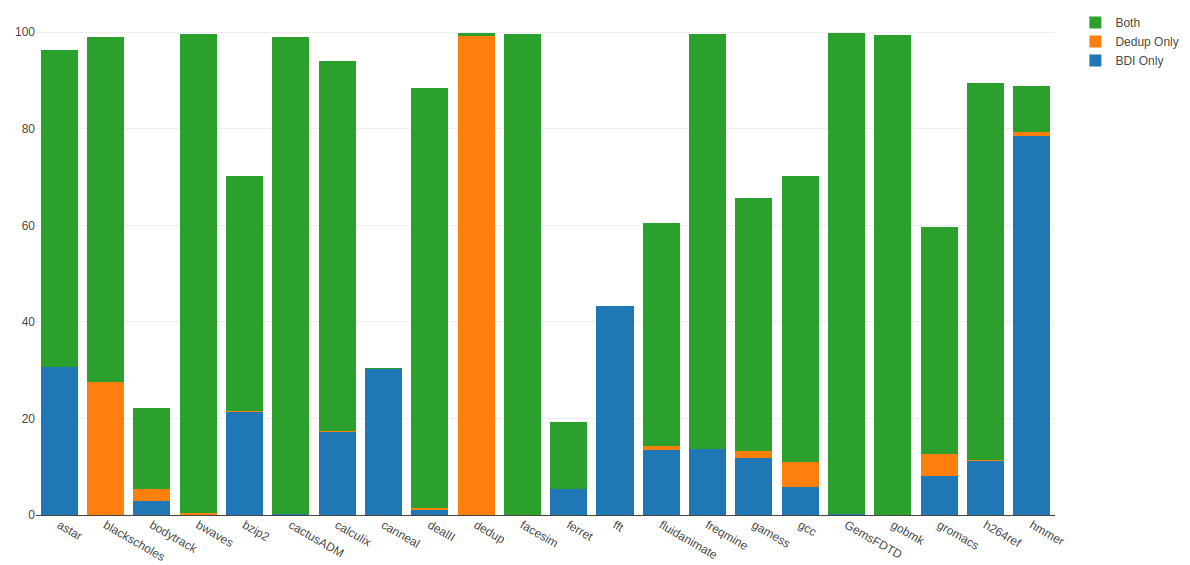
\includegraphics[width=\textwidth]{CompPotential1.png}
    \end{subfigure}
    \begin{subfigure}[b]{\textwidth}
        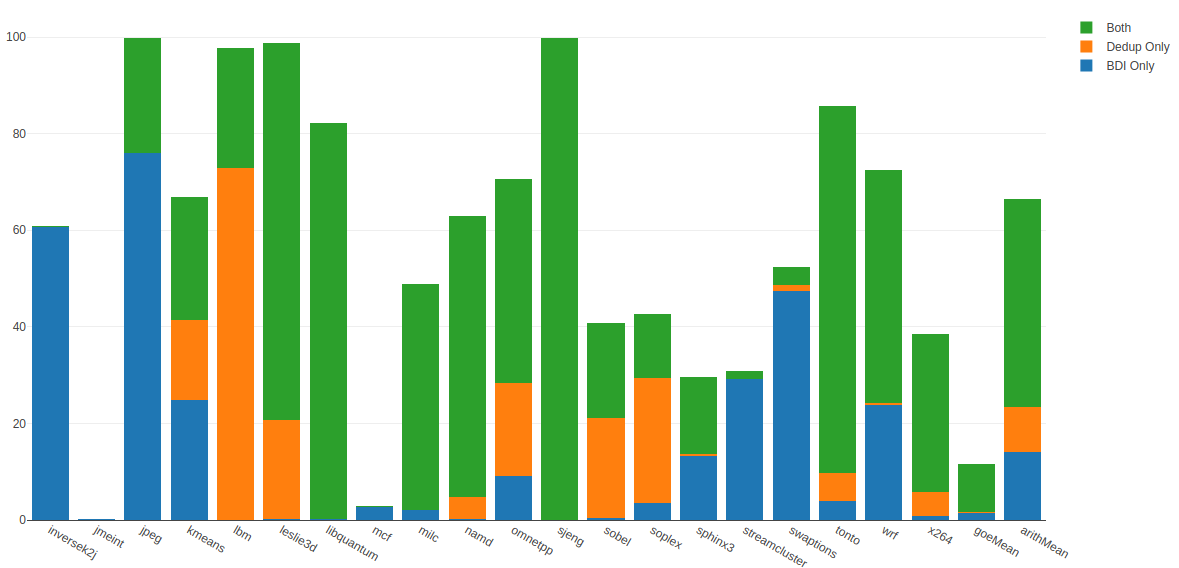
\includegraphics[width=\textwidth]{CompPotential2.png}
    \end{subfigure}
    \caption[Compressible lines]{The figure shows the percentage of cache lines that can be compressed using Dedup, BDI, or both techniques combined together.}
    \label{fig:CompPossibility}
\end{figure}
Generalizing on what we found. We used the same cache dumps to create Figure \ref{fig:CompPossibility} showing the percentage of cache lines that can be compressed by BDI, the percentage of cache lines that are similar and thus deduplicable, and the percentage of cache lines that can be compressed using both schemes.\par
As Figure \ref{fig:CompPossibility} shows, BDI and Deduplications are orthogonal to some degree. The existence of some cache lines that can be compressed by only one of both compression schemes means they can work separately without affecting each other. However, because there are lines that can be compressed by both schemes, BDI can lose some of it's improvements because of deduplication. For example, if ten lines were similar and compressible by BDI, using BDI will compress each of them on it's own, using deduplication will reduce all ten lines to only one line. Using both techniques means deduplication still compresses ten lines to one, but BDI now compresses only one line instead of 10. The improvements of BDI can thus be limited by deduplication.\par
\begin{figure}
    \begin{subfigure}[t]{\textwidth}
        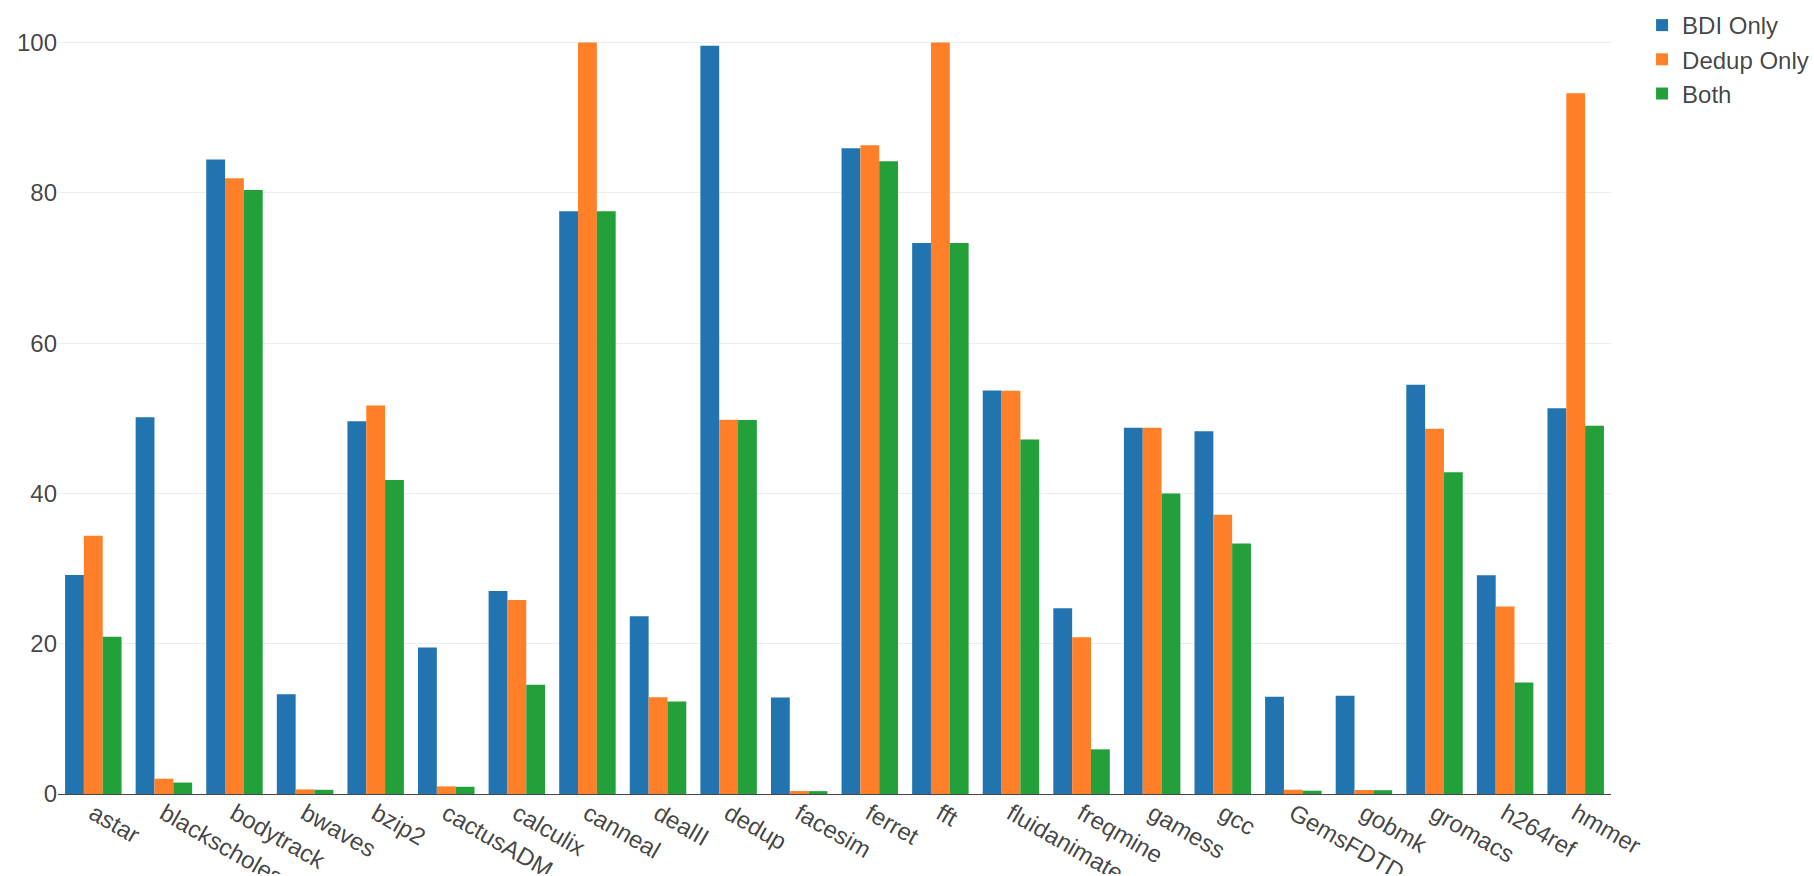
\includegraphics[width=\textwidth]{CompSize1.png}
    \end{subfigure}
    \begin{subfigure}[b]{\textwidth}
        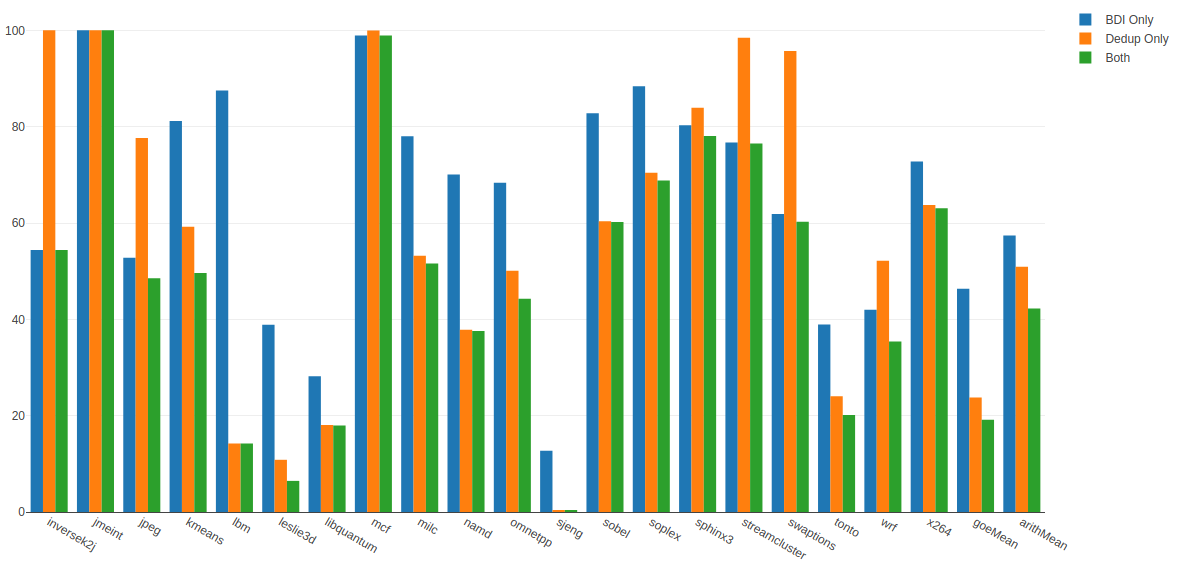
\includegraphics[width=\textwidth]{CompSize2.png}
    \end{subfigure}
    \caption[Size after compression]{The figure shows the size of data in a cache after using compression. BDI, Dedup, and a combination of both is shown.}
    \label{fig:CompSize}
\end{figure}
Nevertheless, combining BDI and Deduplication can still outperform each of them on its own. Figure \ref{fig:CompSize} shows the compressed data size when using BDI, Dedup, and Dedup+BDI. In its worst case Dedup+BDI performs the same as the best out of Dedup and BDI, in most cases it compresses even more on both. Note that the experiments used to create Figure \ref{fig:CompSize} are done statically on cache dumps and thus are completely missing the time dimension and its effect on compression. As time passes more requests to data lines can occur, with more requests the probability that compression can occur increases allowing for better compression.

%% The following is a directive for TeXShop to indicate the main file
%%!TEX root = diss.tex

\chapter{Design}
\label{ch:Design}



%%%%%%%%%%%%%%%%%%%%%%%%%%%%%%%%%%%%%%%%%%%%%%%%%%%%%%%%%%%%%%%%%%%%%%
%%
%% Naive Implementation
%%
%%%%%%%%%%%%%%%%%%%%%%%%%%%%%%%%%%%%%%%%%%%%%%%%%%%%%%%%%%%%%%%%%%%%%%
\section{Straightforward Implementation}
\label{sec:Straightforward Implementation}
In this section we propose an implementation of a cache that combines inter-line and intra-line compression techniques, this implementation is built simply by combining \hyperref[sec:Dedup]{Dedup} and \hyperref[sec:BDI]{BDI}, this cache is thus able to perform deduplication on BDI compressed blocks and uses the same infrastructure and a similar replacement policy to \hyperref[sec:Dedup]{Dedup}.

\subsection{Structure}
\label{ssec:DedupBDIStructure}
\begin{figure}
    \makebox[\textwidth][c]{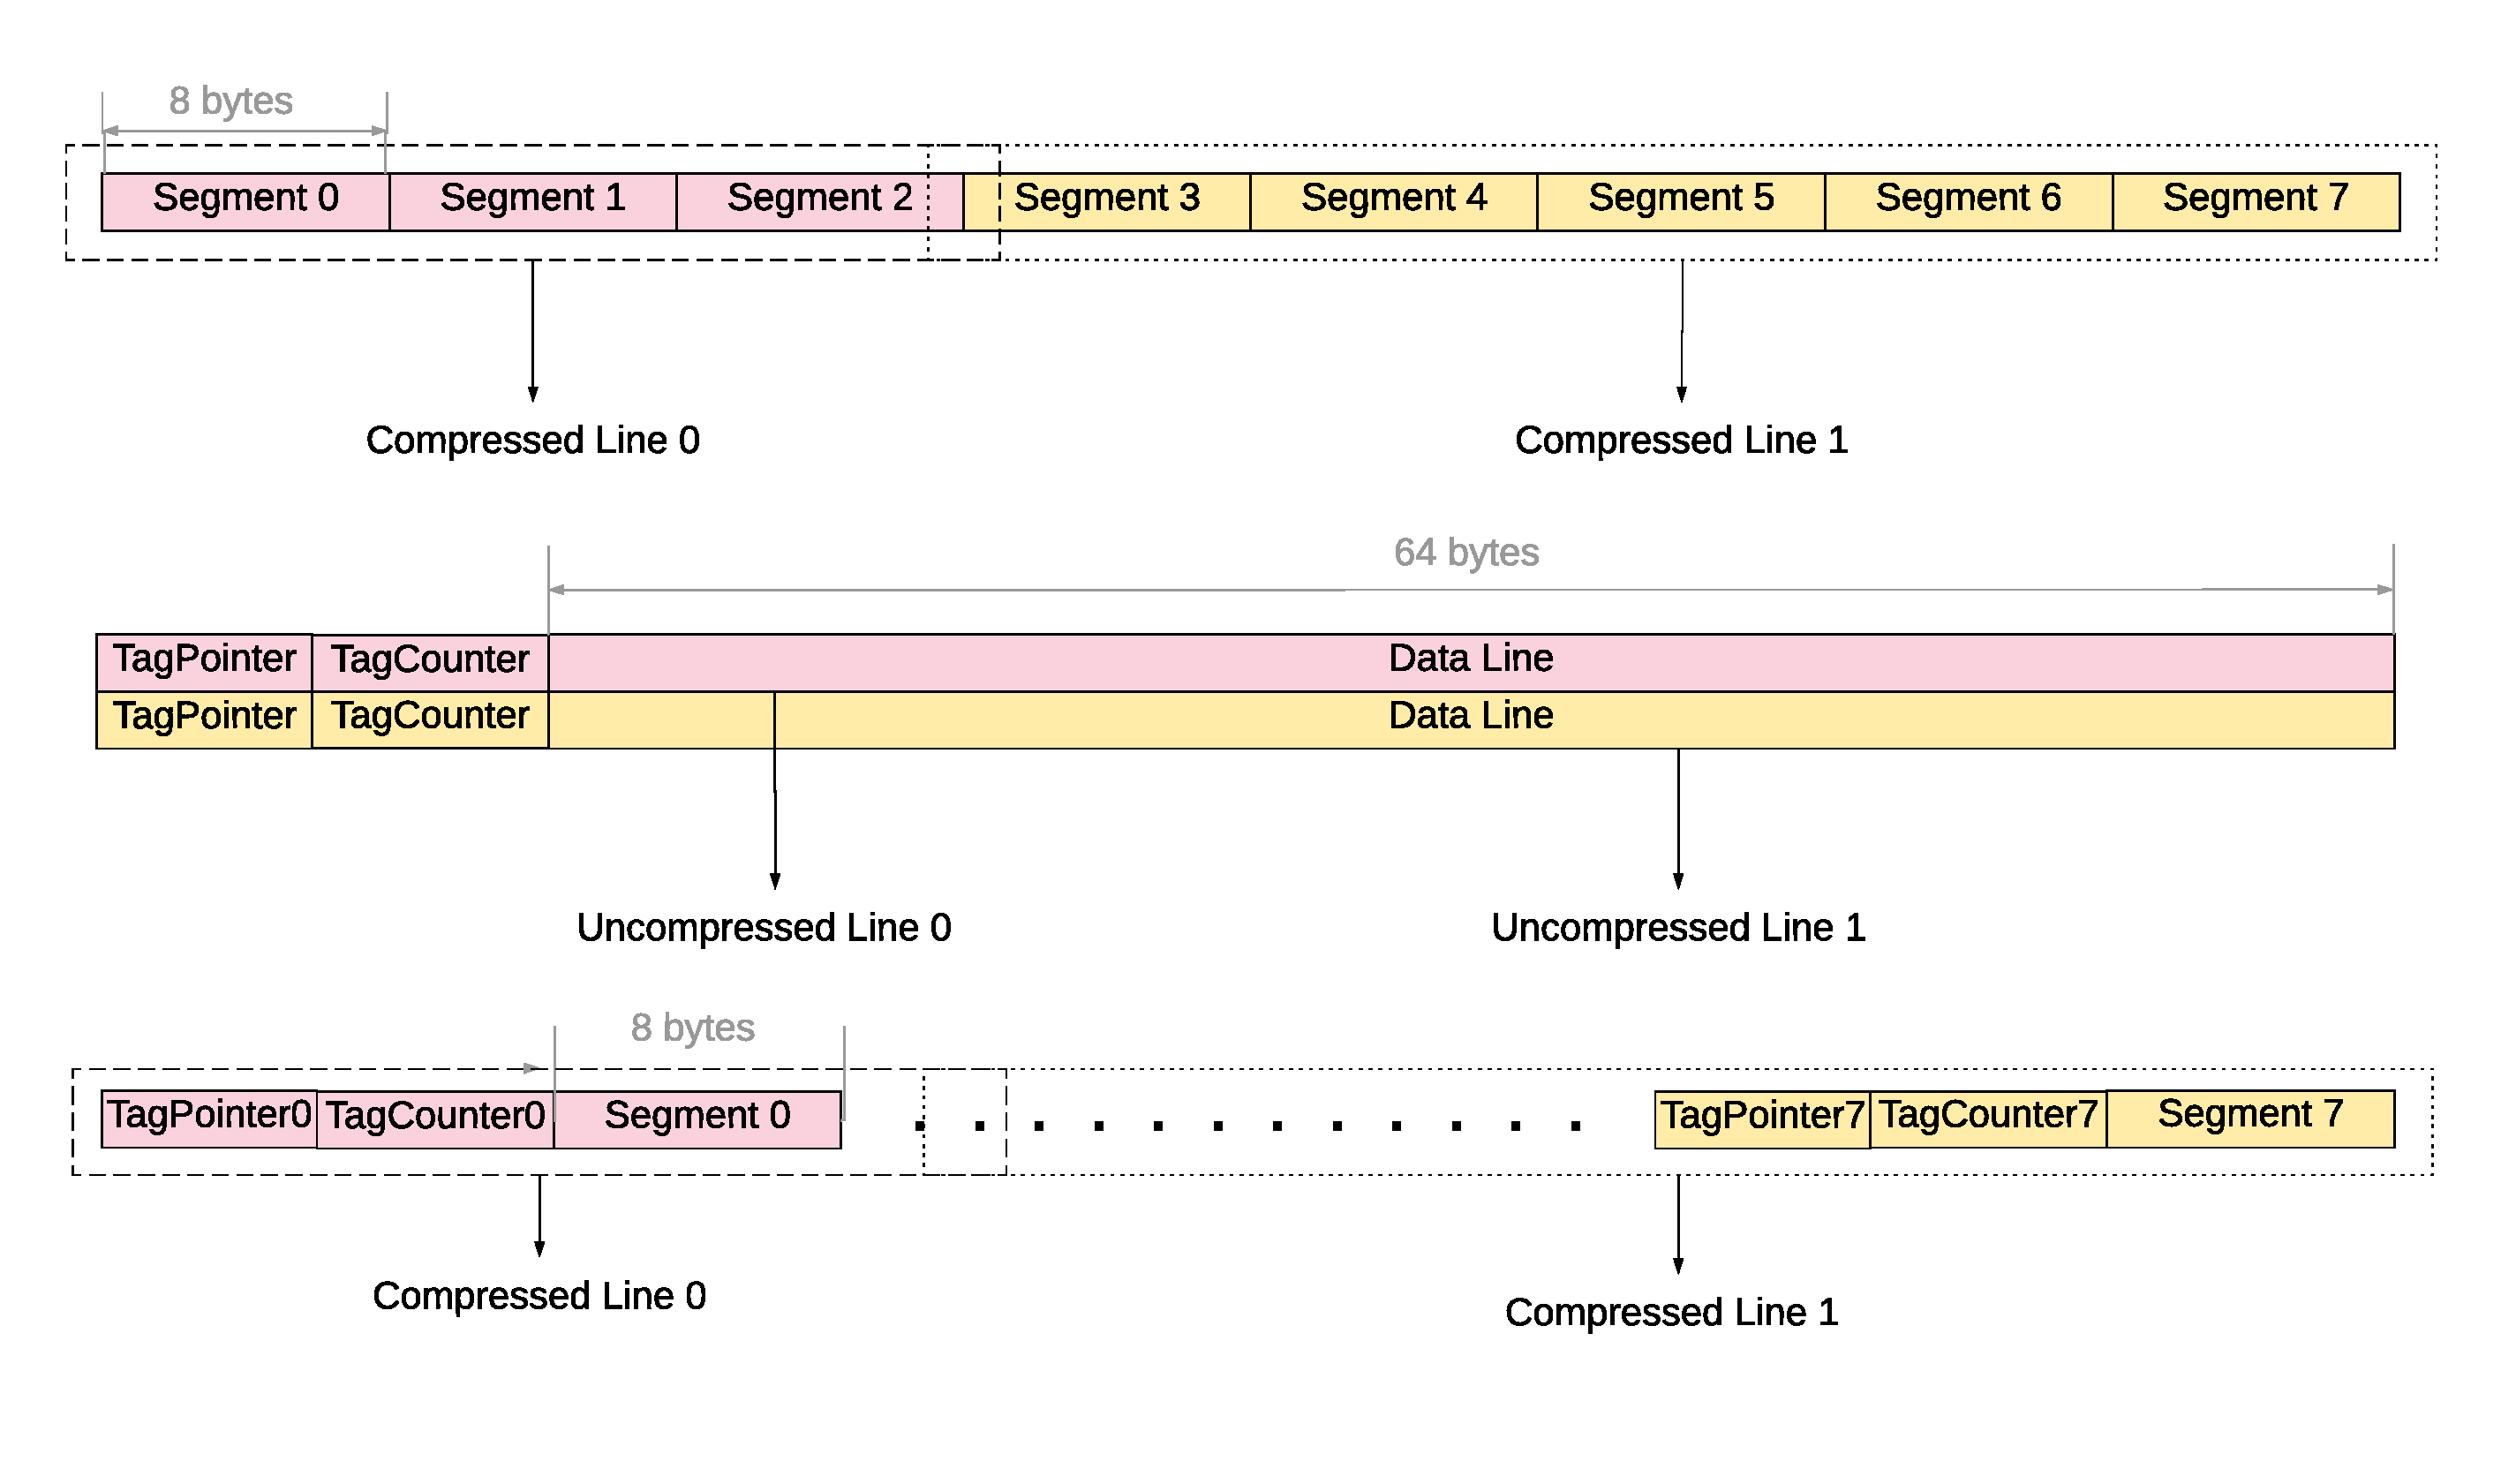
\includegraphics[width=1.5\textwidth]{BDIvsDedupvsDedupBDI_Data.pdf}}
    \label{fig:DedupBDI_Data}
    \caption[DedupBDI Data Array]{The figure shows three different data lines from the BDI, Dedup, and DedupBDI Caches. A data line in a BDI cache can be logically divided into 8 segments, a compressed data line can be represented by one to eight segments, and the data line doesn't hold any metadata. A data line in Dedup cache can only hold uncompressed data lines, so it needs its full 64 byte size, also since it's decoupled from its tag array it needs a tag pointer to be able to point to the tags associated with it, and a counter for its deduplication. A data line in a DedupBDI cache is a combination of both, it needs to be able to hold deduplicated compressed lines, so like a BDI data line it's also divided into 8 segments, but since each segment can hold a compressed line on its own, each segment must have space for the same metadata as a Dedup data line. If a group of segments represent a compressed line, only the metadata of the fist segment in the group is used.}
\end{figure}
\begin{figure}
    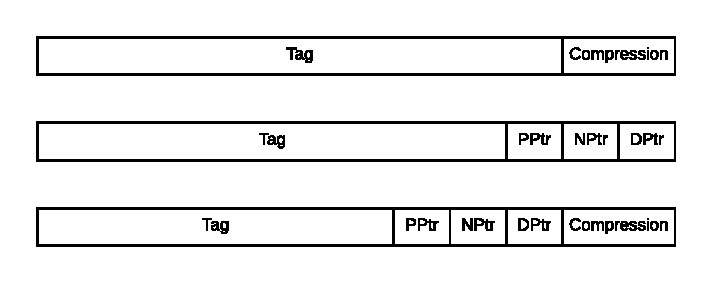
\includegraphics[width=\textwidth]{BDIvsDedupvsDedupBDI_Tag.pdf}
    \label{fig:DedupBDI_Tag}
    \caption[DedupBDI Tag Array]{The figure shows three tag lines from the BDI, Dedup, and DedupBDI Caches. In a BDI cache, tags and data sets are coupled, so each tag needs to know how big is the comressed data associated with it and where it begins, each tag has an extra metadata field that encodes the compression and its size. A Dedup cache allows multiple tags to have the same data line, those tags must be arranged in a linked list so each tag has a previous and a next pointer, all tags have a data pointer to point to their respective data line. In DedupBDI a tag entry must be able to allow deduplication as long as deal with compressed data lines, thus it has the same metadata as a tag entry of a BDI and Dedup cache. The data pointer in DedupBDI must be wider to allow a granularity of data segments not just data lines.}
\end{figure}
\begin{figure}
    \makebox[\textwidth][c]{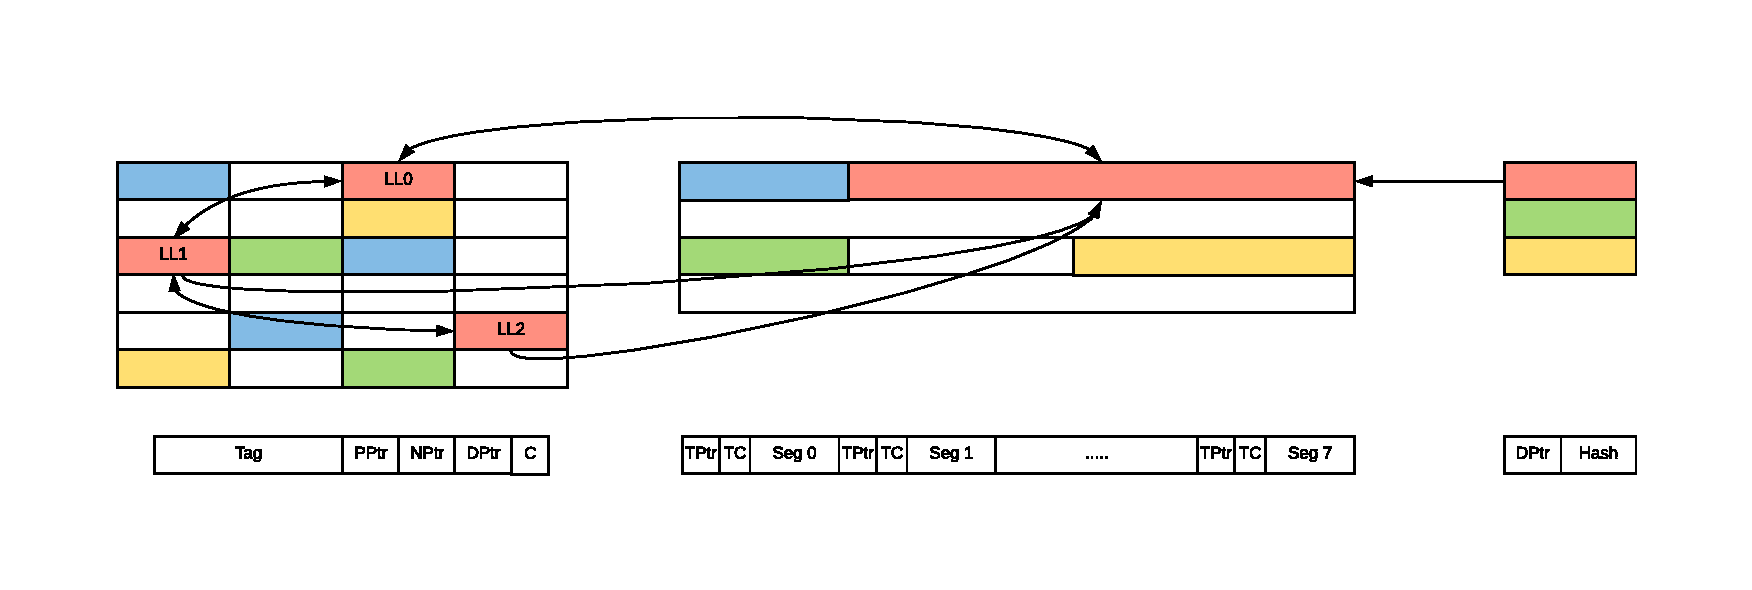
\includegraphics[width=1.5\textwidth]{DedupBDI.pdf}}
    \label{fig:DedupBDI}
    \caption[DedupBDI Cache]{General structure of a DedupBDI Cache, tags that have the same data line are organized together in a linked list using previous and next pointers (PPtr \& NPtr) and they all point to their compressed data line using DPtr and save it's compression data, the compressed data line in return only points to the head tag of the linked list using TPtr and keeps count of how many tags are associated with it using TCount, the hashes in the hash array point to corresponding compressed data lines, if any.}
\end{figure}
The cache consists of three arrays:
%\begin{itemize}
%    \item \textbf{Tag Array: } is a normal tag array, in addition to saving compression and deduplication metadata. Decoupled from the data array, tags connect to data lines through pointers.
%    \item \textbf{Data Array: } is a normal data array that must be able to handle compressed data lines, data lines connect to their tags through pointers.
%    \item \textbf{Hash Array: } used to save hashes of data lines saved in the data array, the hashes facilitate finding similar lines and deduplication
%\end{itemize}
a tag array, a data array, and a hash array. Unlike a normal cache and similar to a \hyperref[sec:Dedup]{Dedup} cache, the tag and data arrays are decoupled and do not have a one to one mapping, instead related tags and data entries have to be able to point to each other. On top of it's normal operation, the tag array is also used to save compression and deduplication metadata. The hash array is needed to facilitate searching for similar data lines to enable deduplication.

The general structure of the cache is shown in Figure \ref{fig:DedupBDI}.
\subsubsection{Tag Array}
\label{sssec:DedupBDITag}
The DedupBDI tag array is a normal, set associative array with no limitations on its associativity or organization. It incorporates extra features from \hyperref[sssec:DedupTag]{Dedup} and \hyperref[sssec:BDITag]{BDI} to support dealing with deduplicated and compressed data lines. Deduplication in its essence means that multiple tags that have similar data lines will be allowed to only save one copy of this data, this breaks the conventional one to one relationship between tags and data in a normal cache making the tag and data caches decoupled. Because of this, a tag entry needs an extra pointer to its corresponding data entry, unlike \hyperref[sssec:DedupTag]{Dedup tag array}'s data pointer, this pointer needs to be able to point to compressed data lines that are smaller in size than normal cache lines, the pointer essentially needs to be larger in size to be able to address lines of smaller granularity. It is actually divided into two pointers: a data set pointer, and a segment pointer, allowing the tag to point to a compressed line anywhere withing the data array boundaries. The tag entries also need to save compression encoding to be able to resolve the size of the compressed data it points to. Similarly to \hyperref[sssec:DedupTag]{Dedup}, tag entries that share the same deduplicated data line are arranged in a linked list, facilitating their eviction in case that data line is evicted. So each tag entry has two extra previous/next pointers to allow them to form a linked list, those pointers need to be big enough to point to tag sets, since reading a tag requires reading the whole set, the required tag from that set can be resolved by comparing it's data pointer. The use of a linked list is necessary in case of data line eviction. In general, the tag array must have more tag entries than the data array, otherwise it wouldn't be able to utilize compression and deduplication. The structure and difference between tag entries in Dedup, BDI, and DedupBDI is shown in Figure \ref{fig:DedupBDI_Tag}
\subsubsection{Data Array}
\label{sssec:DedupBDIData}
The DedupBDI data array is similar to that of a \hyperref[sssec:BDIData]{BDI} cache, each data line in the DedupBDI data array is logically divided into eight segments of eight bytes each (assuming a 64 byte cache line), a compressed data line can occupy any number of segments between one and eight, in the best case scenario all lines will be compressed into one segment each. The data array is decoupled from the tag array because it must also support deduplication, In case a compressed data line is evicted, all the tags associated with it must also be evicted, the compressed data line then must be able to point to the tag linked list and to know how long that list is. Accounting for the best case scenario where each line is compressed into one segment, each segment must have two metadata fields: a pointer to the head of the tag linked list that's associated with this line, and a counter of the tags in that linked list. Both those fields are useful in case an eviction of a data line happens. The pointer needs to be big enough to only point to a tag set, the target tag from this set can be known by comparing its data pointer. The counter only needs to be two bits large, it represents zero/one/two/more, in cases of eviction it can be determined if the count is less than 3 by checking only one tag entry for previous and next pointers. The structure and difference between tag entries in Dedup, BDI, and DedupBDI is shown in Figure \ref{fig:DedupBDI_Data}
\subsubsection{Hash Array}
\label{sssec:DedupBDIHash}
The hash array is a simple set associative structure, it's used to store hashes of some of the data lines providing a way to facilitate finding similar lines and deduplicate them. It is the same as that of a \hyperref[sssec:DedupHash]{Dedup} cache. When a data line is hashed the hash is split into two parts, one is used to index the hash array, while the other is saved in the hash array itself, similar to the tag part of the address being saved in data array. With each entry in the hash array there's also a pointer to a data line that meets this hash, just like the data pointers in the tag array, the pointer is actually two parts, one points to the data set, and the other to the segment in that set. The hash itself is computed like \hyperref[sssec:DedupHash]{Dedup}, through an XOR tree, based on experiments done in \cite{tian2014last} this is enough to keep hash collisions less than 1%.

\subsection{Operations}
\label{ssec:DedupBDIOperations}
\begin{figure}
    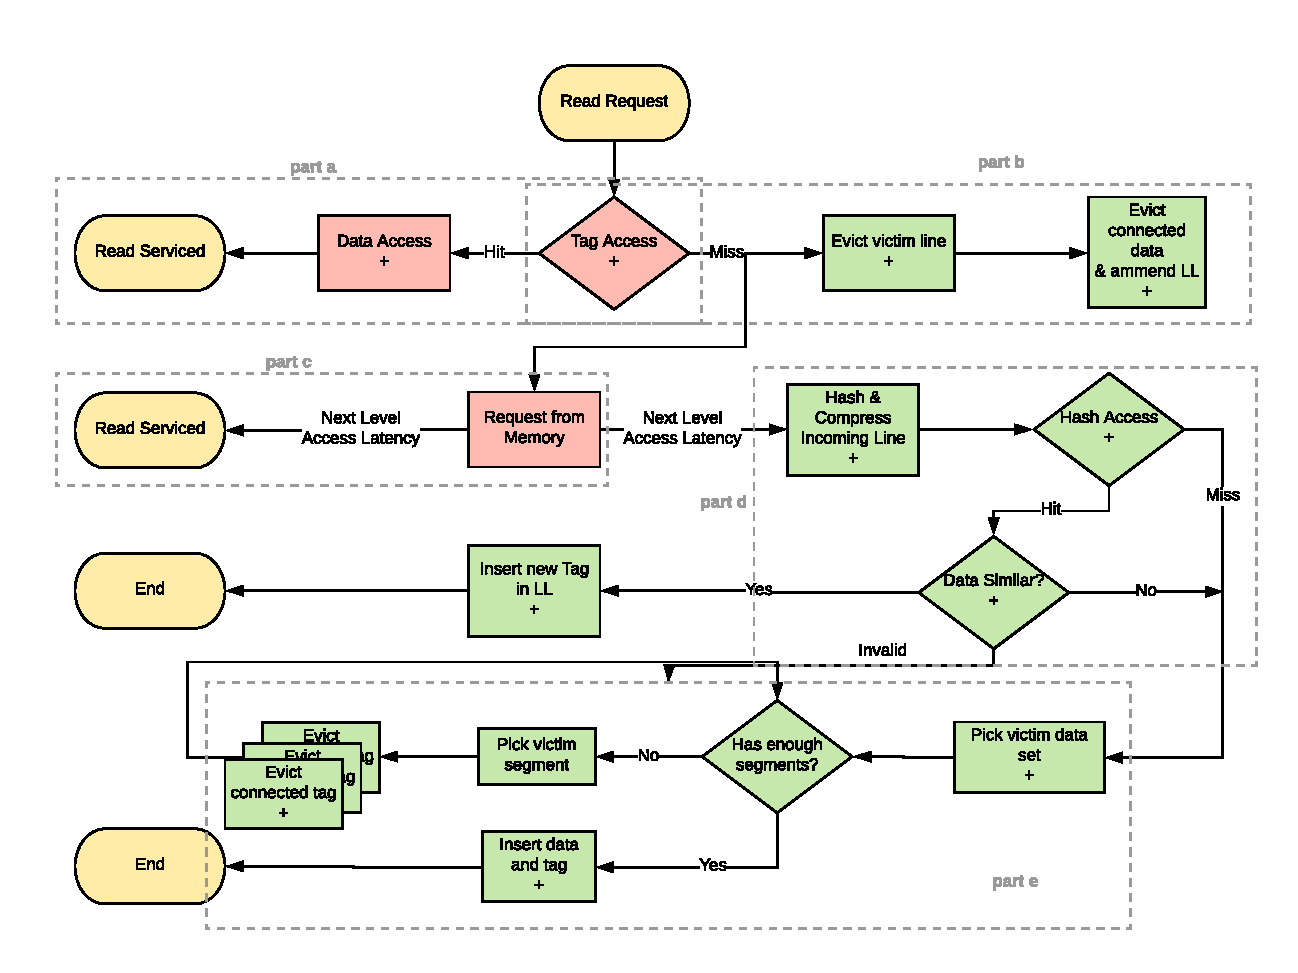
\includegraphics[width=\textwidth,height=\textheight]{DedupBDI_Read.pdf}
    \label{fig:DedupBDI_Read}
    \caption[DedupBDI Read]{Read access flowchart.}
\end{figure}
\begin{figure}
    \contcaption{The flowchart shows the sequence of actions triggered by a read access to the DedupBDI cache. Red blocks signify actions happening on the critical path, while green blocks mean actions happening off the critical path. The blue shaded blocks are actions happening off the critical path but only exist in the straightforward implementation and not the final one. Each + sign in any of the blocks signifies an extra latency for tag array access, data array access, or compression}
\end{figure}
\begin{figure}
    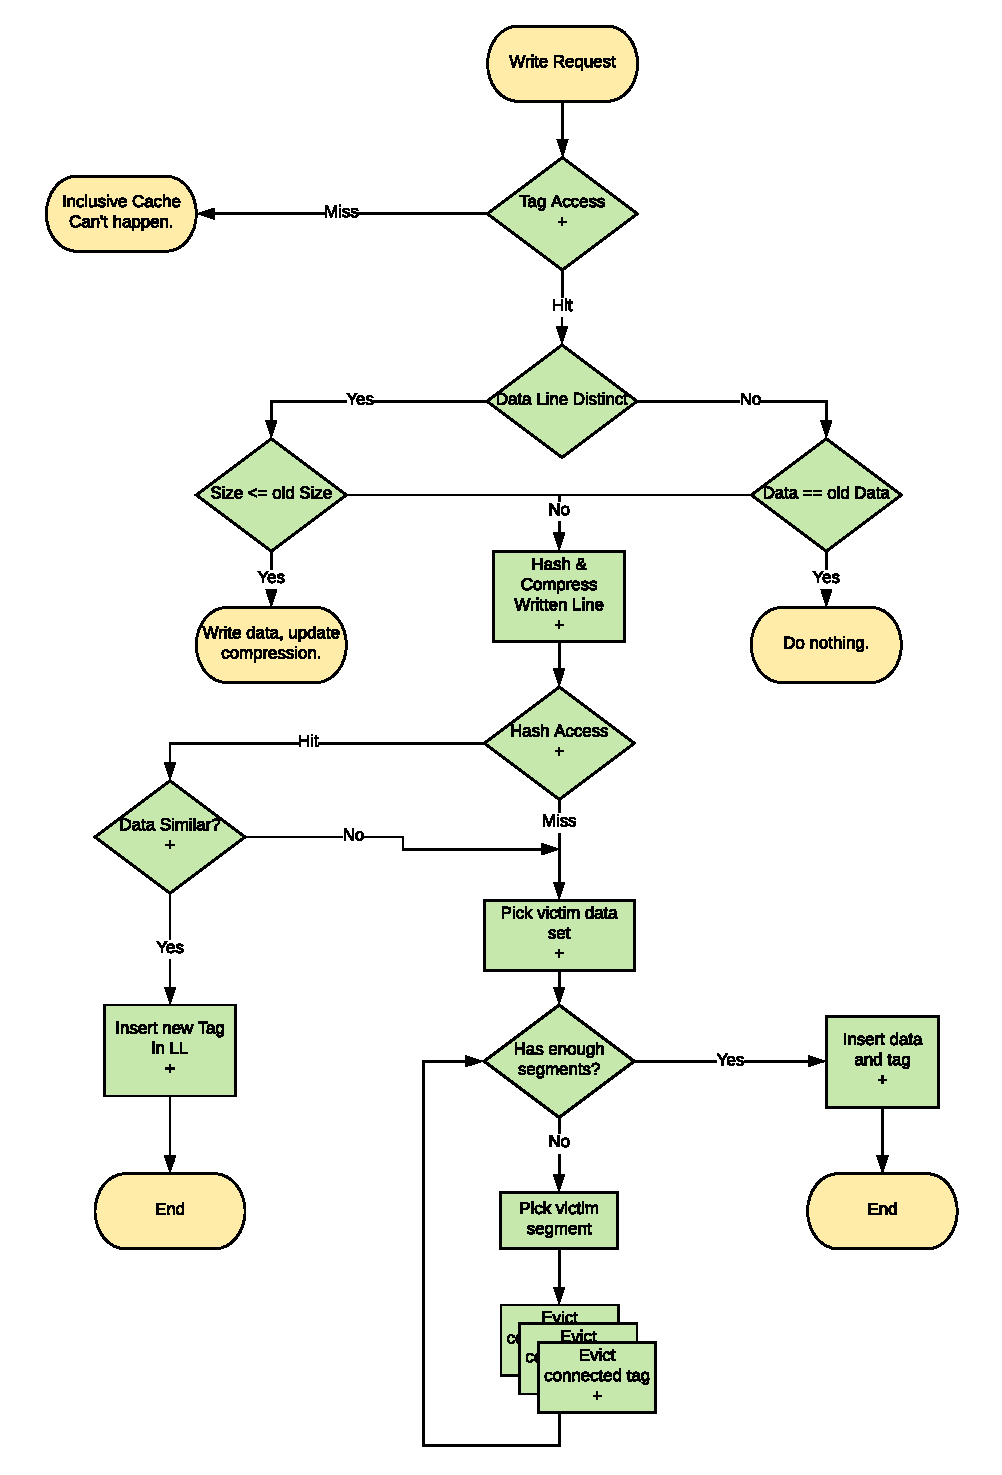
\includegraphics[width=\textwidth,height=\textheight]{DedupBDI_Write.pdf}
    \label{fig:DedupBDI_Write}
    \caption[DedupBDI Write]{Write access flowchart.}
\end{figure}
\begin{figure}
    \contcaption{The flowchart shows the sequence of actions triggered by a write access to the DedupBDI cache. All the blocks are shaded in green because any write request should be off the critical path of the processor regardless of it's status in the cache (hit or miss). The blue shaded blocks are actions happening off the critical path but only exist in the straightforward implementation and not the final one. Each + sign in any of the blocks signifies an extra latency for tag array access, data array access, or compression}
\end{figure}

\subsubsection{Tag Miss}
%% TODO: Cite something for the cache inclusion?
We always assume inclusive caches, so a write request can never miss. On a read tag miss, just like a normal cache, a request for the missed address is forwarded to the next cache level. Meanwhile a victim tag line has to be selected according to the tag replacement policy (e.g. LRU) and evicted if necessary. This eviction may or may not trigger a data line eviction, depending on whether the tag was single (no deduplication) or part of a linked list (deduplication), if the tag is part of linked list then the tags before and after it have to be updated (i.e. Have to point to each other instead of pointing to the victim).

Once the requested line is received, it can be used to service the miss request right away, then placement of the new line can start off the critical path. The received line is first hashed and BDI compressed, the hash is used to compare against the existing hash array, if it hits then the received line has to be compared against the line pointed to by the hash entry, this is needed to make sure because the lines could be different but their hashes are similar (i.e. Hash collision). There are four possible outcomes for this scenario, similar to \hyperref[sssec:DedupOperations]{Dedup}:
\begin{itemize}
    \item \textbf{Hash Miss:} No similar hash is found, either because similar lines do not exist in the data array, or because the hash array is not big enough to keep track of all data lines. In this case we use the data replacement policy to evict victim data line(s) until a sufficient area for the compressed line exists. The new tag is inserted and the tag and data lines have to point to each other, the tag will not point to other tags and will not create a linked list because no deduplication is happening yet. A new hash entry will be selected based on the hash replacement policy and will point to the newly inserted data line.
    \item \textbf{Hash Hit, Line Similar:} In which case the received data line can be deduplicated, it will use the same data line and hash entry. Only the new tag needs to be inserted, it's inserted as the head of the linked list and points to the deduplicated data line. The data line's tag counter (deduplication counter) has to be incremented and it has to pint to the new linked list head.
    \item \textbf{Hash Hit, Line Invalid:} Because hashes point to data lines, but data lines do not point to hashes, when a data line is evicted, it's associated hash might not, causing a situation like this to arise. In this case, we utilize the invalid space right away instead of consulting the data replacement policy. This is similar to the same case in \hyperref[sssec:DedupOperations]{Dedup} with one minor difference, if the invalid space is not enough for the compressed line, we use the data replacement policy to start evicting from the current data set until a sufficient area is enough for the compressed data line to be inserted. The tag entry is also inserted, it has to point to the data line, but it doesn't point to any other tags because the data line is not deduplicated yet and shouldn't have a linked list associated with it. The data line in return also has to point to the tag entry, the hash entry is not changed because it already points to the space we used for the data line.
    \item \textbf{Hash Hit, Line Different:} This case happens only on a hash collision, once a collision happens, it's treated like a hash miss with one modification, a new hash insertion is not needed, the same hash entry will be changed to point to the newly inserted data line in only if the line it was previously pointing to was not deduplicated (i.e. Its tag counter is 1), otherwise it remains untouched. This follows the same policy used in \hyperref[sssec:DedupOperations]{Dedup}.
\end{itemize}
\subsubsection{Tag Hit}
A tag hit has to be treated differently depending on whether it's a read or write request, a read hit is simple, after accessing the tag, the tag's data pointer can be used to access the data line and service the request, a write hit however can be complicated because it can cause the data line to change and thus change it's compressed size and/or hash. If the line was distinct (i.e. Had a tag counter of 1) and the new written size is the same or less than the original size then it can be overwritten right away with the tag updated accordingly, otherwise, the tag disconnects from the data line causing its eviction if it's not deduplicated or causing its counter to decrement and then the request is treated as a tag miss and can follow one of the four cases mentioned above.

\subsection{Replacement Policies}
\label{ssec:Replacement Policies}
Some parts of the DedupBDI cache like the tag array can still operate in the same way with the same replacement policies, the tag array can use one of the known replacement policies like LRU. Other parts of the cache have to be treated differently, since the data and hash array are decoupled from the tag array each one of them needs it's own replacement policy.
\subsubsection{Data Array}
\label{sssec:DedupBDIData}
The data array uses a somewhat similar replacement policy to \hyperref[sssec:DedupDataRepl]{Dedup data replacement policy}, a free list keeping track of free data sets (not lines) is used, whenever needed an entry of this list was used to insert a line. If the list if empty then up to four data sets are picked at random, if any of the sets have enough segments for insertion of the line then it's selected right away, otherwise the one with the least sum of deduplication counters is picked. The picked data set then is used for the second part of the replacement policy, in which a segment (or group of segments representing a compressed data line) with the lowest deduplication counter is selected for eviction, segments keep evicted as necessary until a large enough space is freed for the insertion. Each segment or group of segments evicted can trigger a chain of evictions for the tag linked list associated with it.
\subsubsection{Hash Array}
\label{sssec:DedupBDIHash}
The hash array is indexed by a part of the hash, the selection of a victim hash set is thus dependant on the hash that needs to be inserted, once that set is selected, a hash entry is then selected based on the number of deduplication on the data line it point to, if this data line is not deduplicated then this hash can be used and overwritten, otherwise it's not touched. The rationale behind this is to keep hashes pointing to deduplciated lines from getting evicted and causing the cache to miss extra deduplication for a newly incoming line that might not be useful for deduplication.



%%%%%%%%%%%%%%%%%%%%%%%%%%%%%%%%%%%%%%%%%%%%%%%%%%%%%%%%%%%%%%%%%%%%%%
%%
%% Upper Bound
%%
%%%%%%%%%%%%%%%%%%%%%%%%%%%%%%%%%%%%%%%%%%%%%%%%%%%%%%%%%%%%%%%%%%%%%%
%% TODO: should we discuss "How did we decide what to idealize?". I think we
%% should have a results section for each implementation, to motivate the
%% section after it!
\section{Establishing an Upper Bound}
\label{sec:Upper Bound}
To be able to evaluate the straightforward design we discussed in the previous section, an upper bound must be established, we try to get the upper bound of enhancements by idealizing the design choices we have selected. There are two aspects we can idealize in this design:
\begin{itemize}
    %TODO: Dump data lines, show missed dedup and quantify.
    \item \textbf{Finding a similar line:} Finding a similar line in the DedupBDI cache has two sources of possible error: The first is the hashing itself, because hashing data lines to a smaller space means it will never be perfect and collisions are inevitable. The second limitation is the size of hash array, because the number of entries in the hash array is less than that of the data array, there's a chance that an opportunity for deduplication is missed because the hash array was too small and couldn't keep its hash. Finding a similar line can be idealized by directly searching through the data array and comparing each line until a similar data line is found.
    %TODO: Show figure of data utilization here.
    %TODO: Show L2 Back Invs and use NMRU as ideal instead of LRU?
    \item \textbf{Replacement of data lines:} Imperfections in the replacement policy of data array comes from two sources: the first is the free list, since we cannot make the free list keep track of all free segments in the data array because it would be impractically large, it can only keep track of free sets, that means even if only one segment is used from a set that set is not kept in the free list anymore. The second source is the random selection of data lines whenever the free list is empty, our experiments show that the random selection causes utilization of the data array to be less than a 100\% as shown in \ref{ch:Results}, selecting 4 random sets might now always yield a set with enough free segments, selecting more than 4 can be time inefficient. We idealize the replacement policy by directly searching the whole data cache for free segments that are enough to insert a new compressed line, this ensures a 100\% utilization of the data array, if no free segments are available we use data array wide LRU to pick a victim segment(s) instead of doing it randomly.
\end{itemize}
with the use of perfect deduplication and data insertion, a hash array is no longer needed, and the tag array is no different than a normal cache. The \ref{ch:Results} chapter shows the performance of both the straightforward implementation and the idealized one.



%%%%%%%%%%%%%%%%%%%%%%%%%%%%%%%%%%%%%%%%%%%%%%%%%%%%%%%%%%%%%%%%%%%%%%
%%
%% Final Implementation
%%
%%%%%%%%%%%%%%%%%%%%%%%%%%%%%%%%%%%%%%%%%%%%%%%%%%%%%%%%%%%%%%%%%%%%%%
\section{Final Implementation}
\label{sec:Final Implementation}
In order to improve on the naive implementation and towards the upper bound, we propose the following realistic improvements on the straightforward implementation.
\begin{itemize}
    %TODO: Quantify this
    \item \textbf{Deduplication:} while any realistic deduplication will still depend on the existence of a hash array. The hash array used in the straightforward was the same as \hyperref[sssec:DedupHash]{Dedup}, the hash array was enough to cover deduplications in the data array of \ref{sec:Dedup}, but because of the use of compression in DedupBDI, each line can hold up to eight times the amount of data, the same hash array with the same number of entries might not be enough to cover that amount of deduplication efficiently. In the \ref{ch:Results} we show how varying the number of hash array entries can affect the performance of deduplication in DedupBDI cache.
    \item \textbf{Data free list:} To keep track of all free segments in the data array, a modification to the free list was made, the free list is now divided into multiple free lists, each of which can keep track of data sets with a certain amount of free segments, namely we have eight free lists, the first keeps track of data sets with one free segment and the second with two, until the last which keeps track of data sets with eight or more free segments, whenever a data line needs to be inserted, the free list corresponding to its size is looked up first, if it's empty then the larger ones are searched one by one, if no empty segments exist then we return to the second part of the replacement policy.
    %TODO: Results of L2 back invs.
    %TODO: Need to quantify LRU vs Rand vs NMRU
    %TODO: Quantify how it hurts
    \item \textbf{Replacement of data lines:} Two modifications of the replacement policy were introduced. The first is ignoring the replacement policy in case of a tag miss, hash hit, but invalid data line was found to be hurting the performance as in some cases the space of the invalid line might not be enough but another enough space might exist, the better alternative is to always consult the replacement policy. The second change I cannot write about until I quantify.
\end{itemize}


%% The following is a directive for TeXShop to indicate the main file
%%!TEX root = diss.tex

\chapter{Results}
\label{ch:Results}

In this chapter we show results for the \hyperref[sec:BDI]{BDI}, \hyperref[sec:Dedup]{Dedup}, and \hyperref[sec:Final Implementation]{DedupBDI} caches along with the \hyperref[sec:Upper Bound]{roofline model} we established for DedepBDI. We show how those four cache designs affect compression, MPKI, and speedup.

\section{Methodology}
\label{sec:Methodology}
\begin{table}[]
    \centering
    \begin{tabular}{ll}
        Component & Configuration                                                                                                                                            \\ \hline
        CPU       & x86\_64, 2.6GHz, 4-wide OoO, 80 entry ROB.                                                                                                               \\
        L1I       & 32KB, 4 way, 3 cycle access lat, 64B lines, LRU.                                                                                                         \\
        L1D       & 32KB, 8 way, 4 cycle access lat, 64B lines, LRU.                                                                                                         \\
        L2        & Private, 256KB, 8 way, 11 cycle access lat, 64B lines, LRU.                                                                                              \\
        L3        & \begin{tabular}[c]{@{}l@{}}Shared, 0.5MB-8MB (or similar tag array size if compressed),\\  16 way, 39 cycle access lat, 64B lines, 8 banks.\end{tabular} \\
        Mem       & DDR3-1066, 1GB.                                                                                                                                         
        \end{tabular}
    \caption{The simulated system}
    \label{tab:simsys}
\end{table}
\begin{table}[]
    \centering
    \begin{tabular}{|l|l|l|l|}
    \hline
    Compression                   & Cache & Data Entries & Tag Entries \\ \hline
    \multirow{5}{*}{Conventional} & 0.5MB & 8192         & 8192        \\ \cline{2-4} 
                                  & 1MB   & 16384        & 16384       \\ \cline{2-4} 
                                  & 2MB   & 32768        & 32768       \\ \cline{2-4} 
                                  & 4MB   & 65536        & 65536       \\ \cline{2-4} 
                                  & 8MB   & 131072       & 131072      \\ \hline
    \multirow{5}{*}{COMP-2}       & 0.5MB & 4096         & 8192        \\ \cline{2-4} 
                                  & 1MB   & 8192         & 16384       \\ \cline{2-4} 
                                  & 2MB   & 16384        & 32768       \\ \cline{2-4} 
                                  & 4MB   & 32768        & 65536       \\ \cline{2-4} 
                                  & 8MB   & 65536        & 131072      \\ \hline
    \multirow{5}{*}{COMP-4}       & 0.5MB & 2048         & 8192        \\ \cline{2-4} 
                                  & 1MB   & 4096         & 16384       \\ \cline{2-4} 
                                  & 2MB   & 8192         & 32768       \\ \cline{2-4} 
                                  & 4MB   & 16384        & 65536       \\ \cline{2-4} 
                                  & 8MB   & 32768        & 131072      \\ \hline
    \end{tabular}
    \caption{All cache configurations.}
    \label{tab:simcache}
\end{table}
We used the zsim\cite{zsim} simulator to design and implement the four target caches: BDI, Dedup, DedupBDI, and Ideal DedupBDI along with a baseline conventional (uncompressed) cache. We used an out-of-order core timing model based on a medium-size x86 core, with detailed timing for all critical-path and off-critical-path events. We simulated a system with a 3 level cache hierarchy, with private L1 and L2 caches and a shared L3 cache. The simulated system is listed in Table \ref{tab:simsys}.\par 
We simulated different conventional L3 cache sizes ranging from 0.5MB to 8MB. We also simulated the four compressed caches at the same tag array sizes, but with data arrays half and one quarter of the size. For example, a 4MB-2 BDI cache has the same number of tags as a conventional 4MB cache, but its tag to data ratio is 2 so its data array size is half of its conventional counterpart. The LLC cache configurations are shown in \ref{tab:simcache}. The workloads used are all the benchmarks from the AxBench\cite{axbench} benchmark suite, the Parsec\cite{parsec} benchmark suite with simmedium inputs, and the Spec\cite{spec} benchmark suite with train inputs (mid-size inputs). All the benchmarks were simulated until end or 3 billion instructions.

\section{Case Study}
\label{sec:case_study}
In this section we describe the four benchmarks we picked in \ref{sec:Motivation}. The benchmarks have different cache patterns and behaviors. During the static analysis done in \ref{sec:Motivation} canneal was only compressible by BDI, dedup was compressible using deduplication, jmeint was uncompressible while libquantum was compressible by both. We analyze how these benchmarks behave when simulated in a real computing system with compressed caches.\par
\begin{figure}
    \begin{subfigure}{0.5\textwidth}
        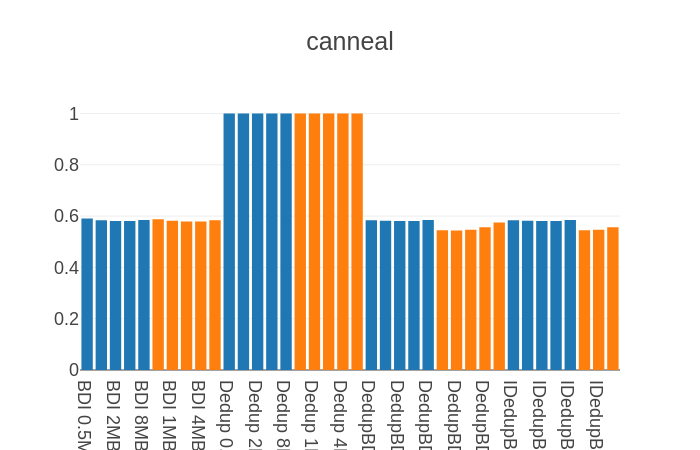
\includegraphics[width=\textwidth]{canneal-compratio.png}
        \caption{canneal}
    \end{subfigure}
    \begin{subfigure}{0.5\textwidth}
        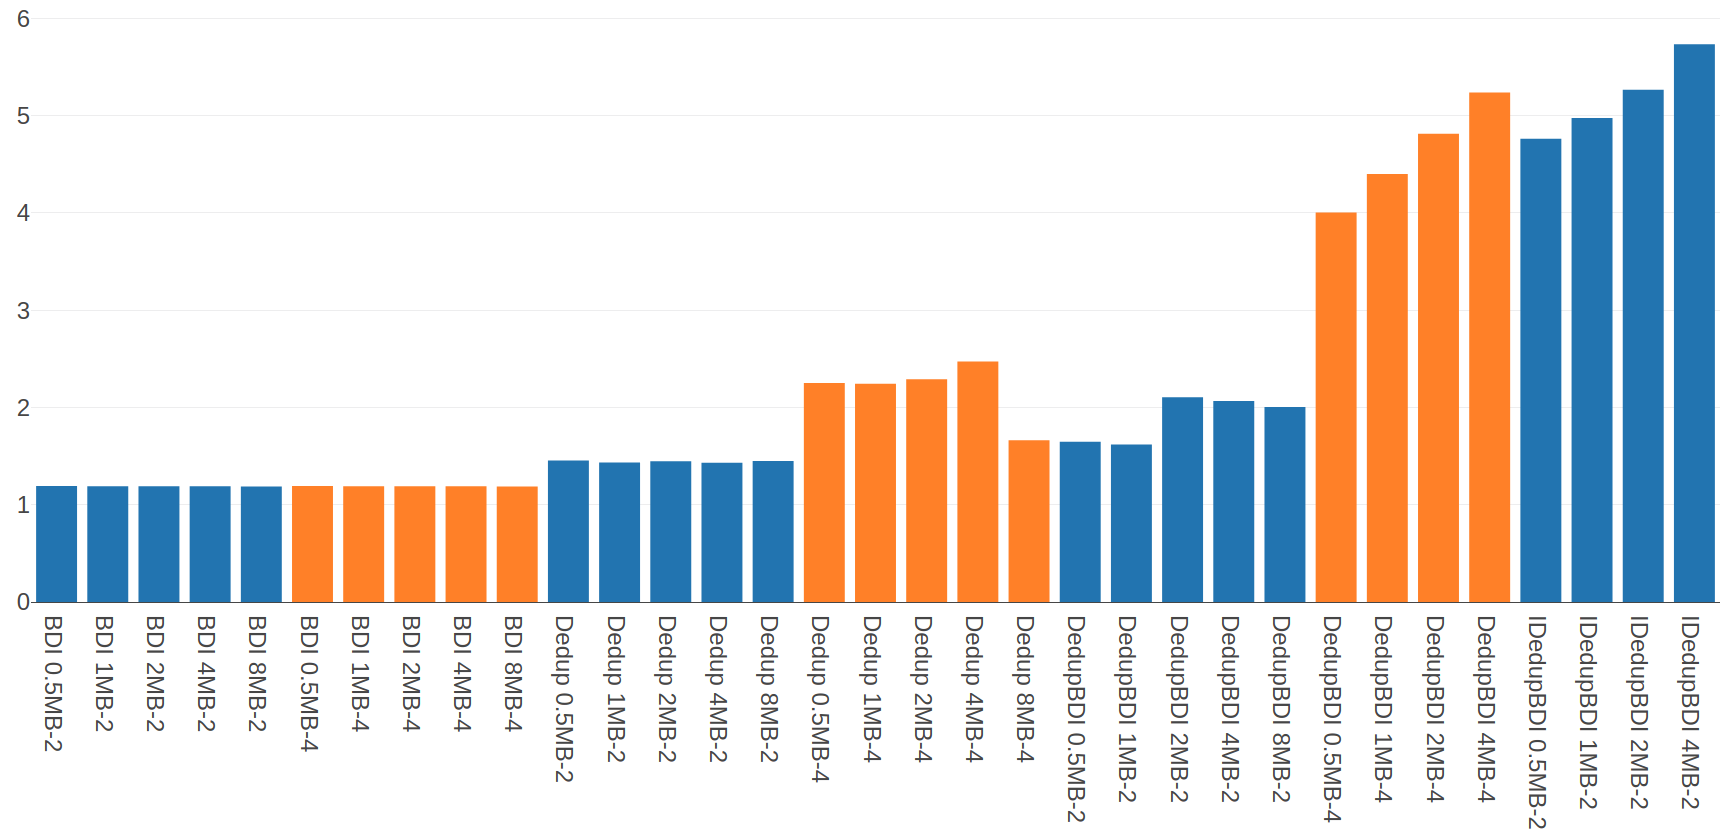
\includegraphics[width=\textwidth]{lbm-compratio.png}
        \caption{lbm}
    \end{subfigure}
    \begin{subfigure}{0.5\textwidth}
        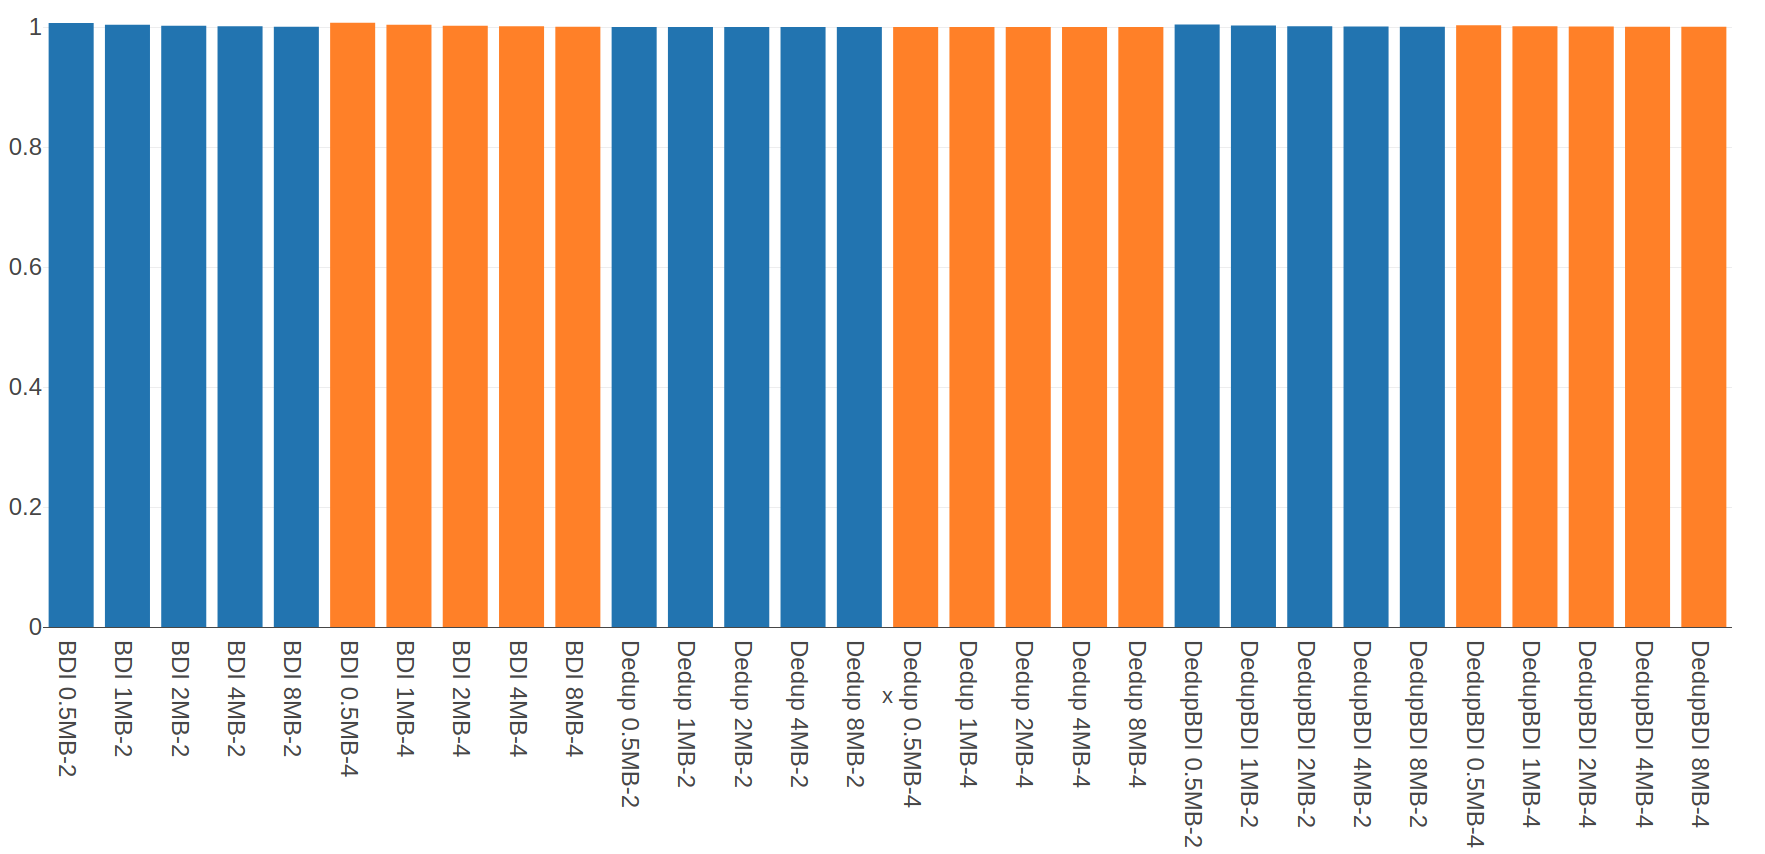
\includegraphics[width=\textwidth]{jmeint-compratio.png}
        \caption{jmeint}
    \end{subfigure}
    \begin{subfigure}{0.5\textwidth}
        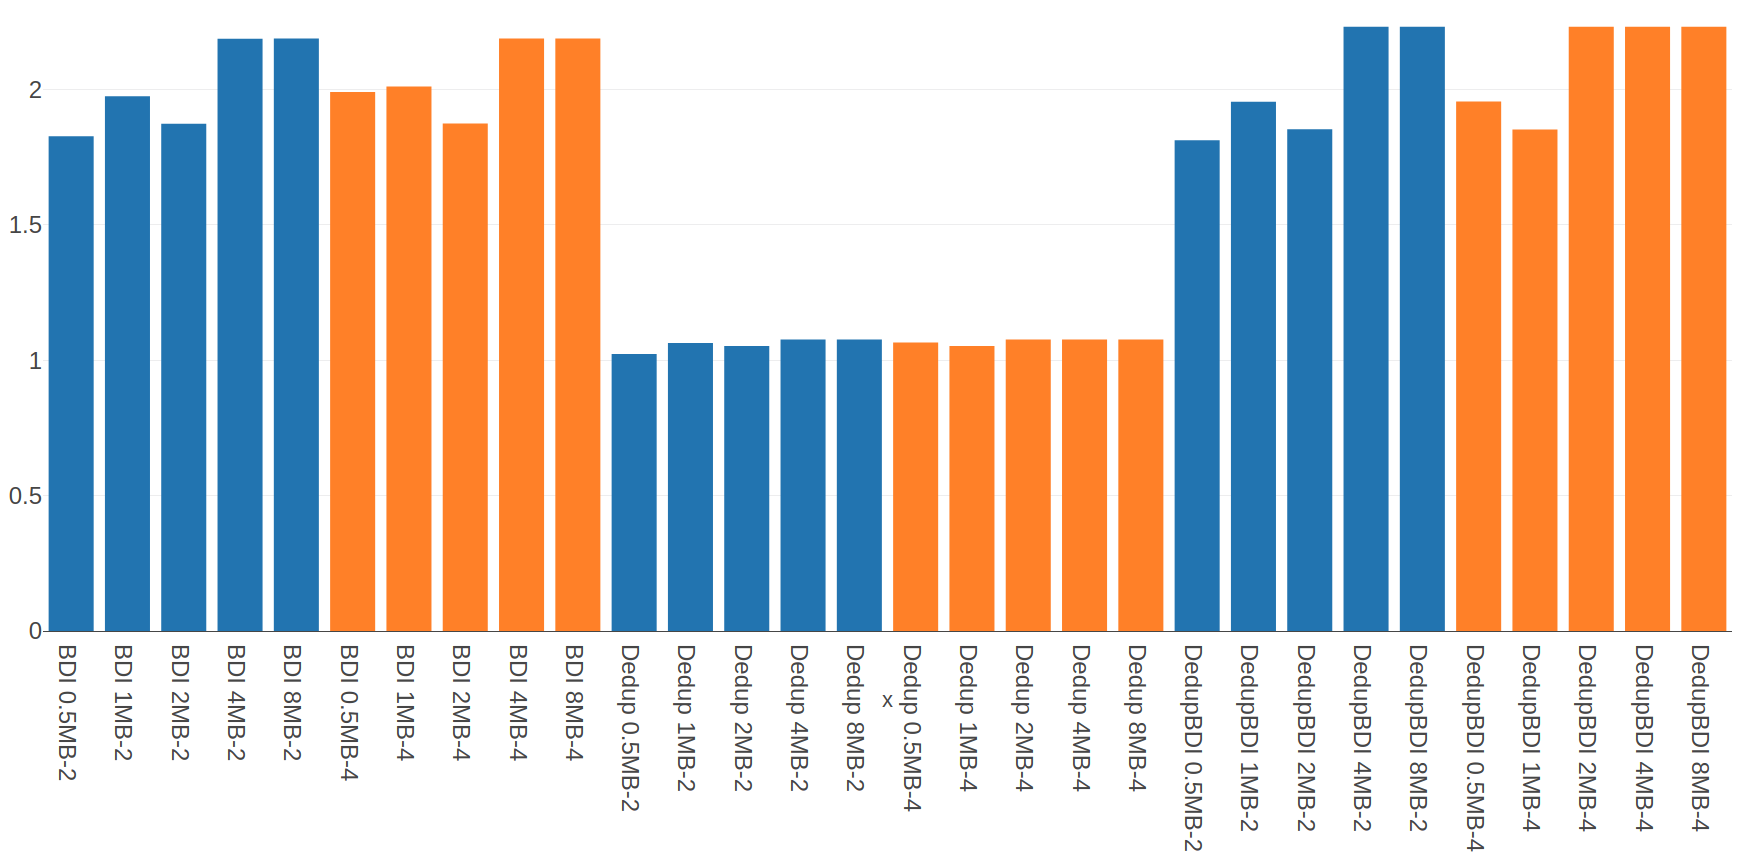
\includegraphics[width=\textwidth]{libquantum-compratio.png}
        \caption{libquantum}
    \end{subfigure}
    \caption[Case Study: Compression]{Showing four benchmarks and their compression ratio using different compressed caches.}
    \label{fig:case_compratio}
\end{figure}
Figure \ref{fig:case_compratio} shows the compression ratio of the four benchmarks. Compression ratio is calculated as the ratio between valid tags and valid data entries. The blue columns are caches with tag entries double the data entries, while the orange ones have tags four times the data entries. As expected, canneal shows some compression with BDI but nothing with Dedup, lbm shows compression using Dedup but not using BDI, jmeint shows no compression using any of the caches, while libquantum shows compression using all of them. The DedupBDI cache combines the best of both worlds and either outperforms or at least does as good as BDI or Dedup.\par
Figures \ref{fig:case_mpki} and \ref{fig:case_speedup} show the MPKI and Speedup for the four benchmarks under all cache configurations. Apart from the incompressible jmeint, all the benchmarks show huge speedups (up to 70\% in case of libquantum). DedupBDI is the best performing cache in canneal, lbm and libquantum. But it's slightly worse (0.01\% slowdown) than a conventional cache in jmeint.
\begin{figure}
    \begin{subfigure}{0.5\textwidth}
        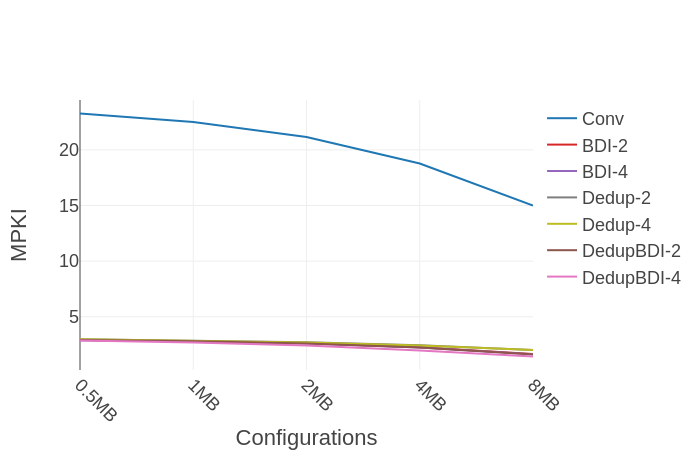
\includegraphics[width=\textwidth]{canneal-mpki.png}
        \caption{canneal}
    \end{subfigure}
    \begin{subfigure}{0.5\textwidth}
        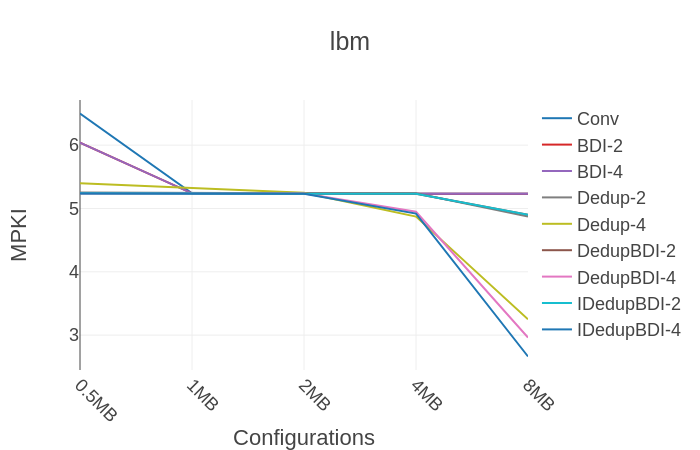
\includegraphics[width=\textwidth]{lbm-mpki.png}
        \caption{lbm}
    \end{subfigure}
    \begin{subfigure}{0.5\textwidth}
        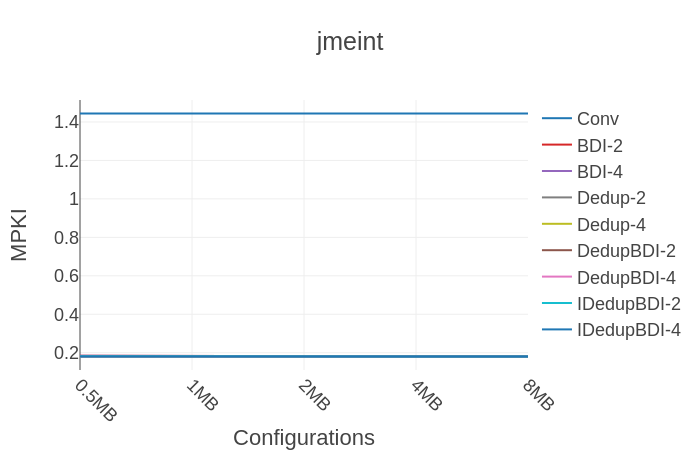
\includegraphics[width=\textwidth]{jmeint-mpki.png}
        \caption{jmeint}
    \end{subfigure}
    \begin{subfigure}{0.5\textwidth}
        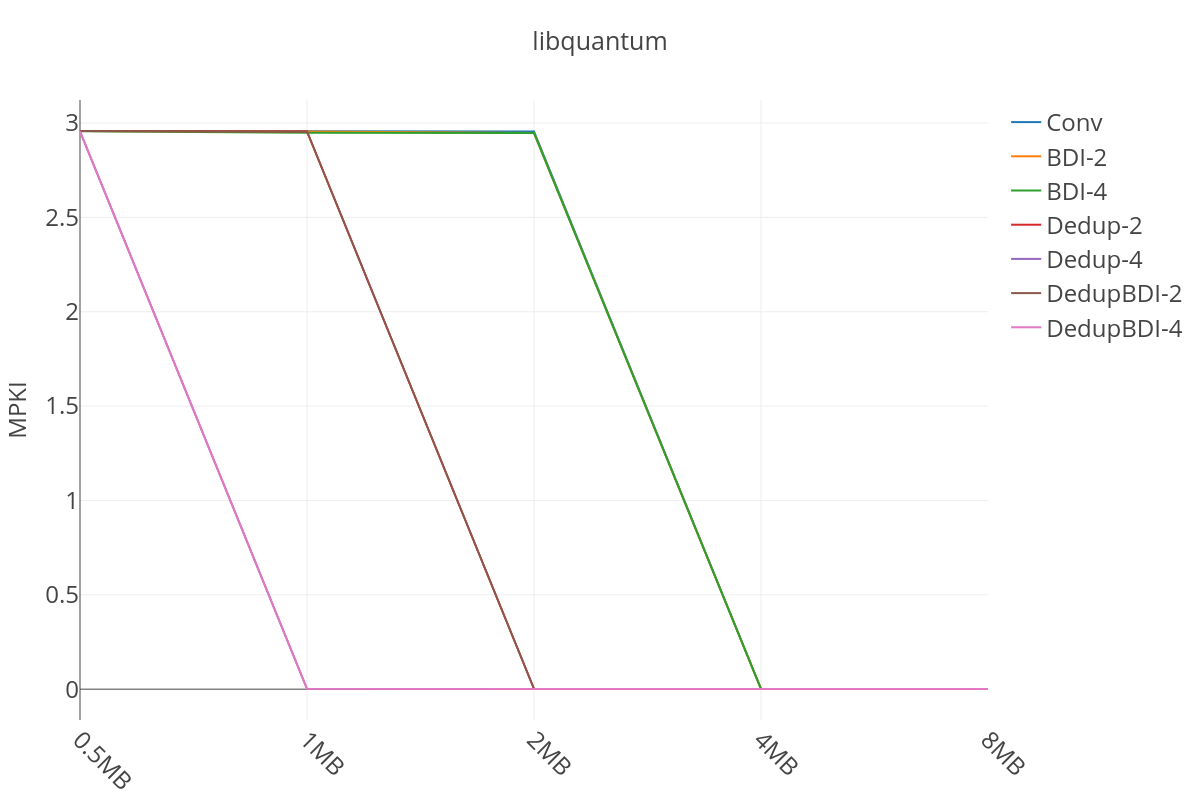
\includegraphics[width=\textwidth]{libquantum-mpki.png}
        \caption{libquantum}
    \end{subfigure}
    \caption[Case Study: MPKI]{Showing four benchmarks and their MPKI using different compressed caches.}
    \label{fig:case_mpki}
\end{figure}
\begin{figure}
    \begin{subfigure}{0.5\textwidth}
        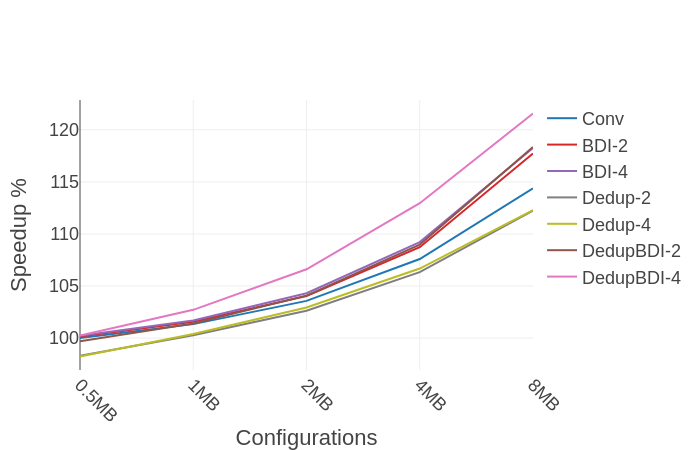
\includegraphics[width=\textwidth]{canneal-speedup.png}
        \caption{canneal}
    \end{subfigure}
    \begin{subfigure}{0.5\textwidth}
        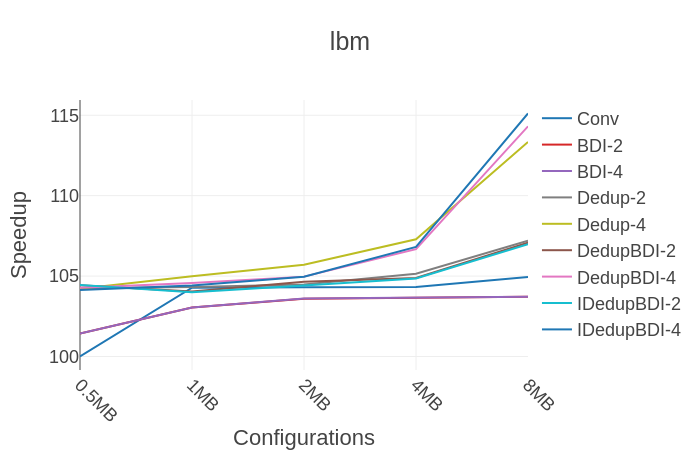
\includegraphics[width=\textwidth]{lbm-speedup.png}
        \caption{lbm}
    \end{subfigure}
    \begin{subfigure}{0.5\textwidth}
        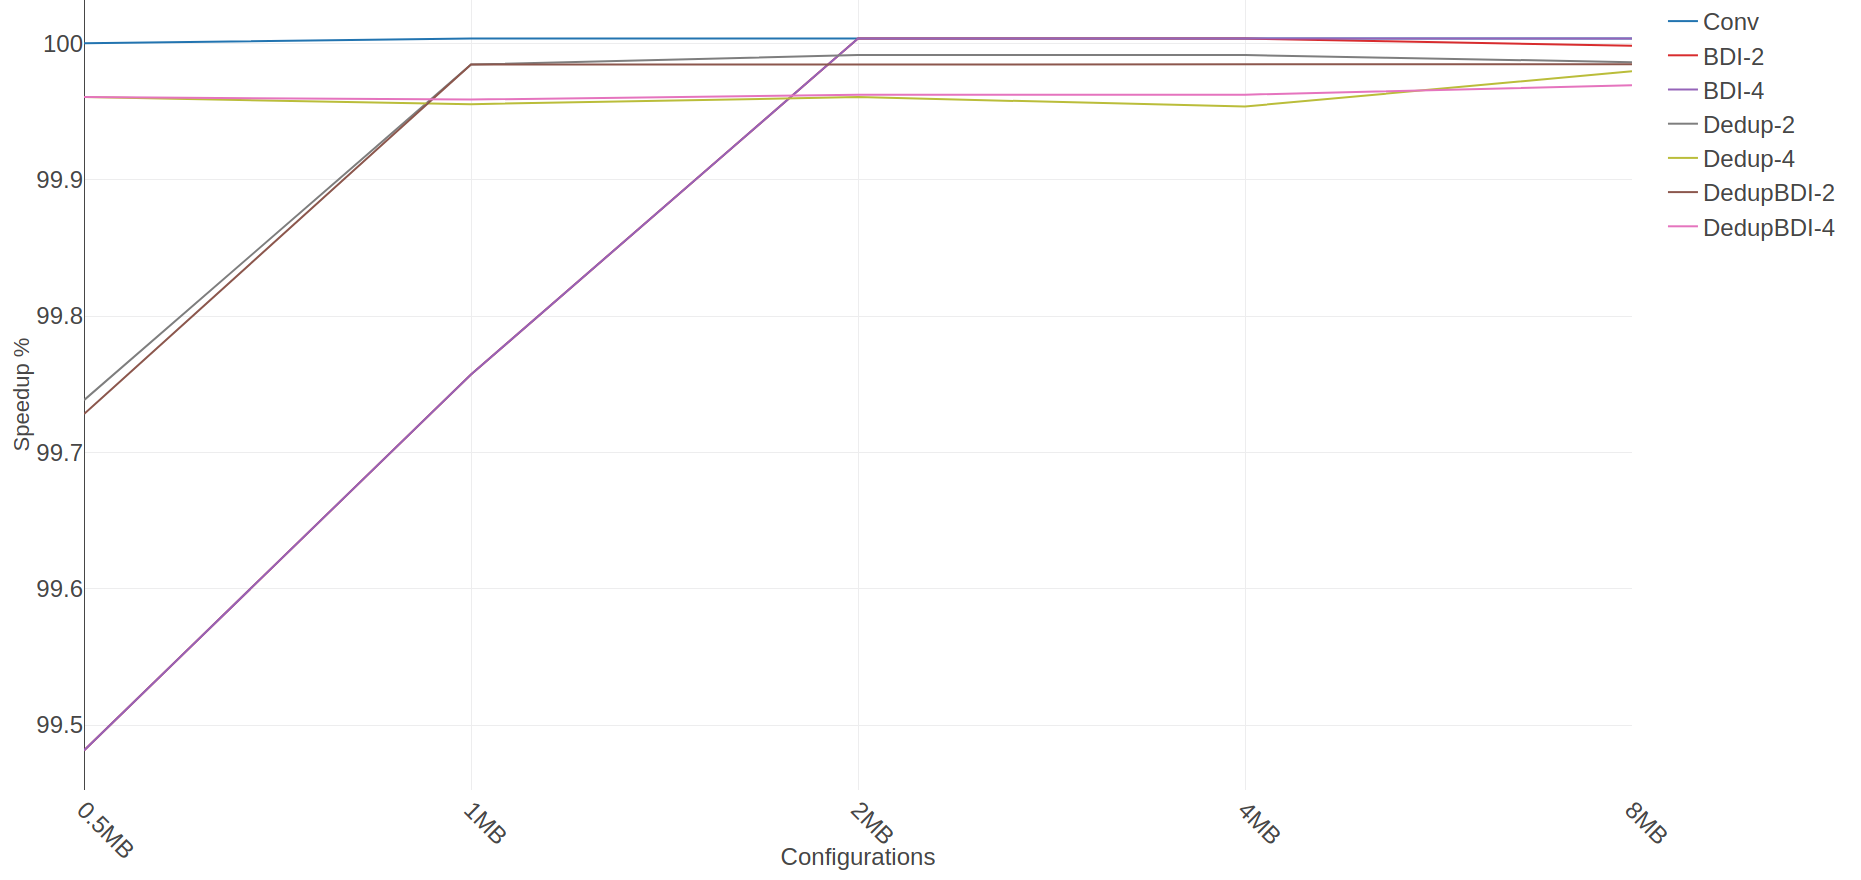
\includegraphics[width=\textwidth]{jmeint-speedup.png}
        \caption{jmeint}
    \end{subfigure}
    \begin{subfigure}{0.5\textwidth}
        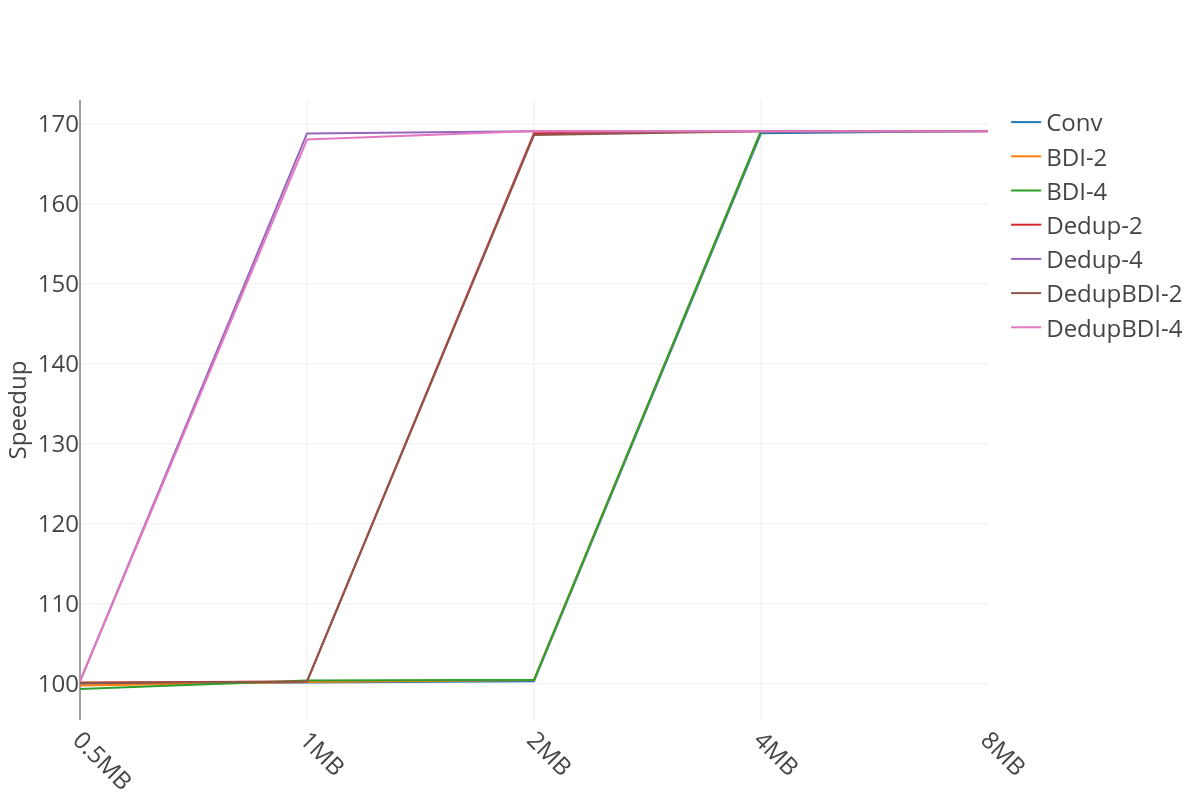
\includegraphics[width=\textwidth]{libquantum-speedup.png}
        \caption{libquantum}
    \end{subfigure}
    \caption[Case Study: Speedup]{Showing four benchmarks and their speedup using different compressed caches.}
    \label{fig:case_speedup}
\end{figure}

\section{Compression}
\label{sec:Compression}
Figure \ref{fig:all_compratio} shows the compression ratio for all the benchmarks when simulated with a compressed 4MB LLC with tags four times the data lines. It's shown that DedupBDI performs either better than BDI and Dedup, or at least similar to the dominant one. There're no cases in which DedupBDI compressed worse than BDI or Dedup.\par
It can also be seen that the difference between DedupBDI and the roofline model (IDedupBDI) is minimal in most cases. Only in bwaves and fft benchmarks the roofline perform a lot better than the real world implementation.\par
However, the compression ratio does not tell the full story. If a cache contains 512 valid tags out of 1024, and 256 valid data lines out of 256 then it has a compression ratio of 0.5 but it's not being fully utilized. Normal conventional caches usually have near 100\% utilization unless the working data set is very small to entirely fit inside a cache. Figure \ref{fig:all_util} shows the tag and data array utilization for all benchmarks. Most of the benchmarks can be divided into two categories:
\begin{itemize}
    \item \textbf{tag limited:} Those are benchmarks that have very high tag utilization, but lower than 100\% data utilization. GemsFDTD is an obvious example. Those benchmarks are highly compressible and thus are bound by the size of the tag array. Evictions in such benchmarks are mainly caused by the tag array replacement policy.
    \item \textbf{data limited:} Those benchmarks reach 100\% utilization of their data arrays before the tag array is full. This is because they have a lower degree of compressibility. Evictions in those benchmarks are prominently caused by the data array replacement policy.
\end{itemize}
\begin{figure}
    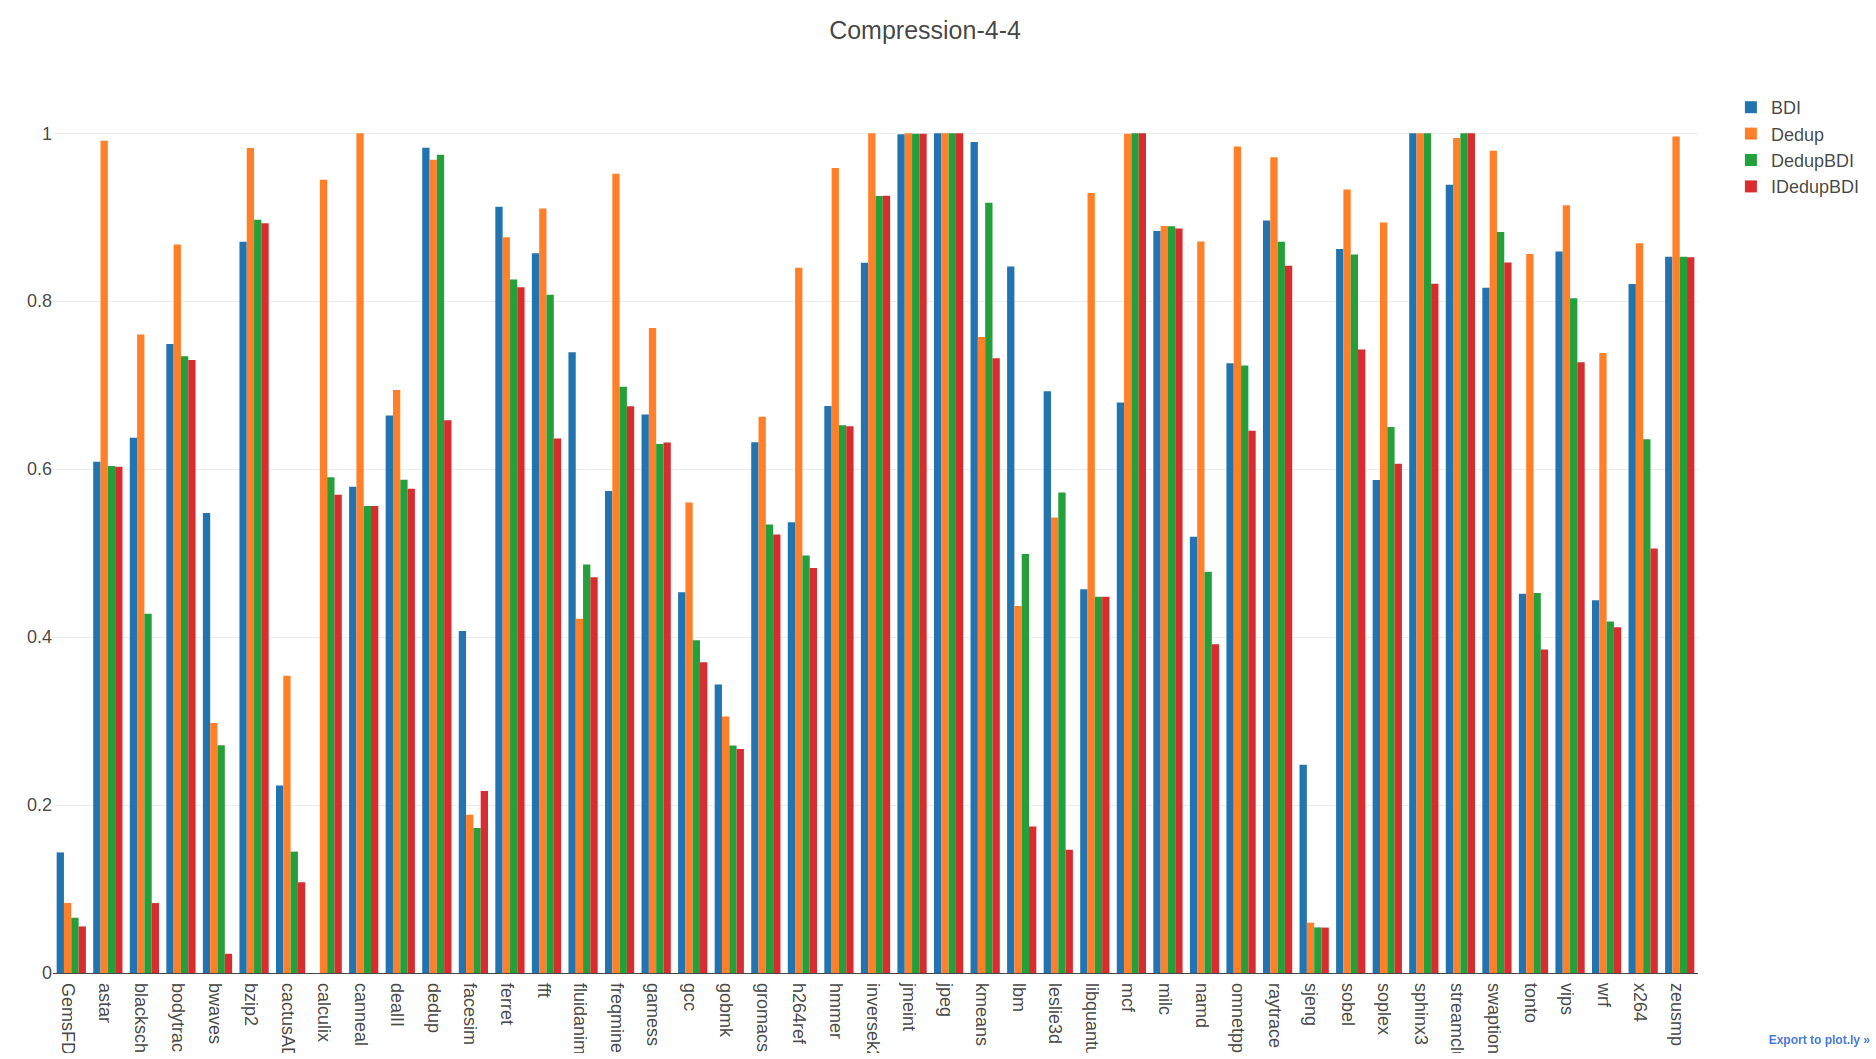
\includegraphics[width=\textwidth]{all-compratio.png}
    \caption[All benchmarks: Compression]{Showing compression ratio for all benchmarks using all types of compressed 4MB caches with tags four times data.}
    \label{fig:all_compratio}
\end{figure}
\begin{figure}
    \begin{subfigure}{\textwidth}
        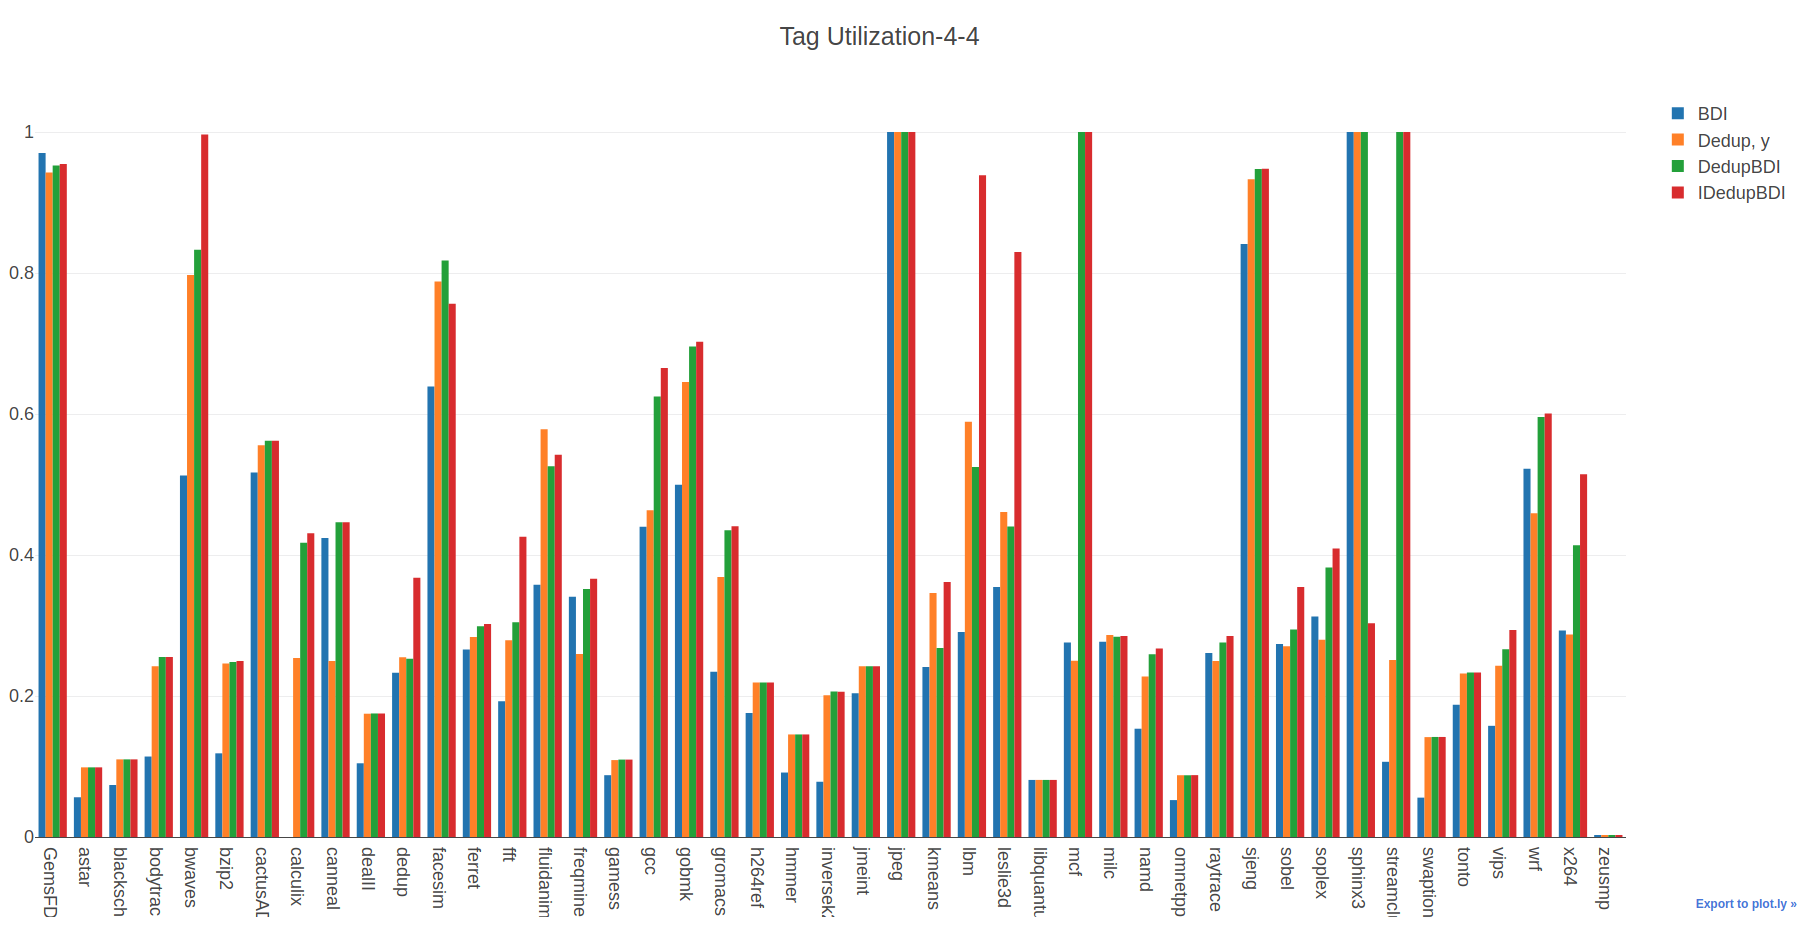
\includegraphics[width=\textwidth]{all-tagutil.png}
    \end{subfigure}
    \begin{subfigure}{\textwidth}
        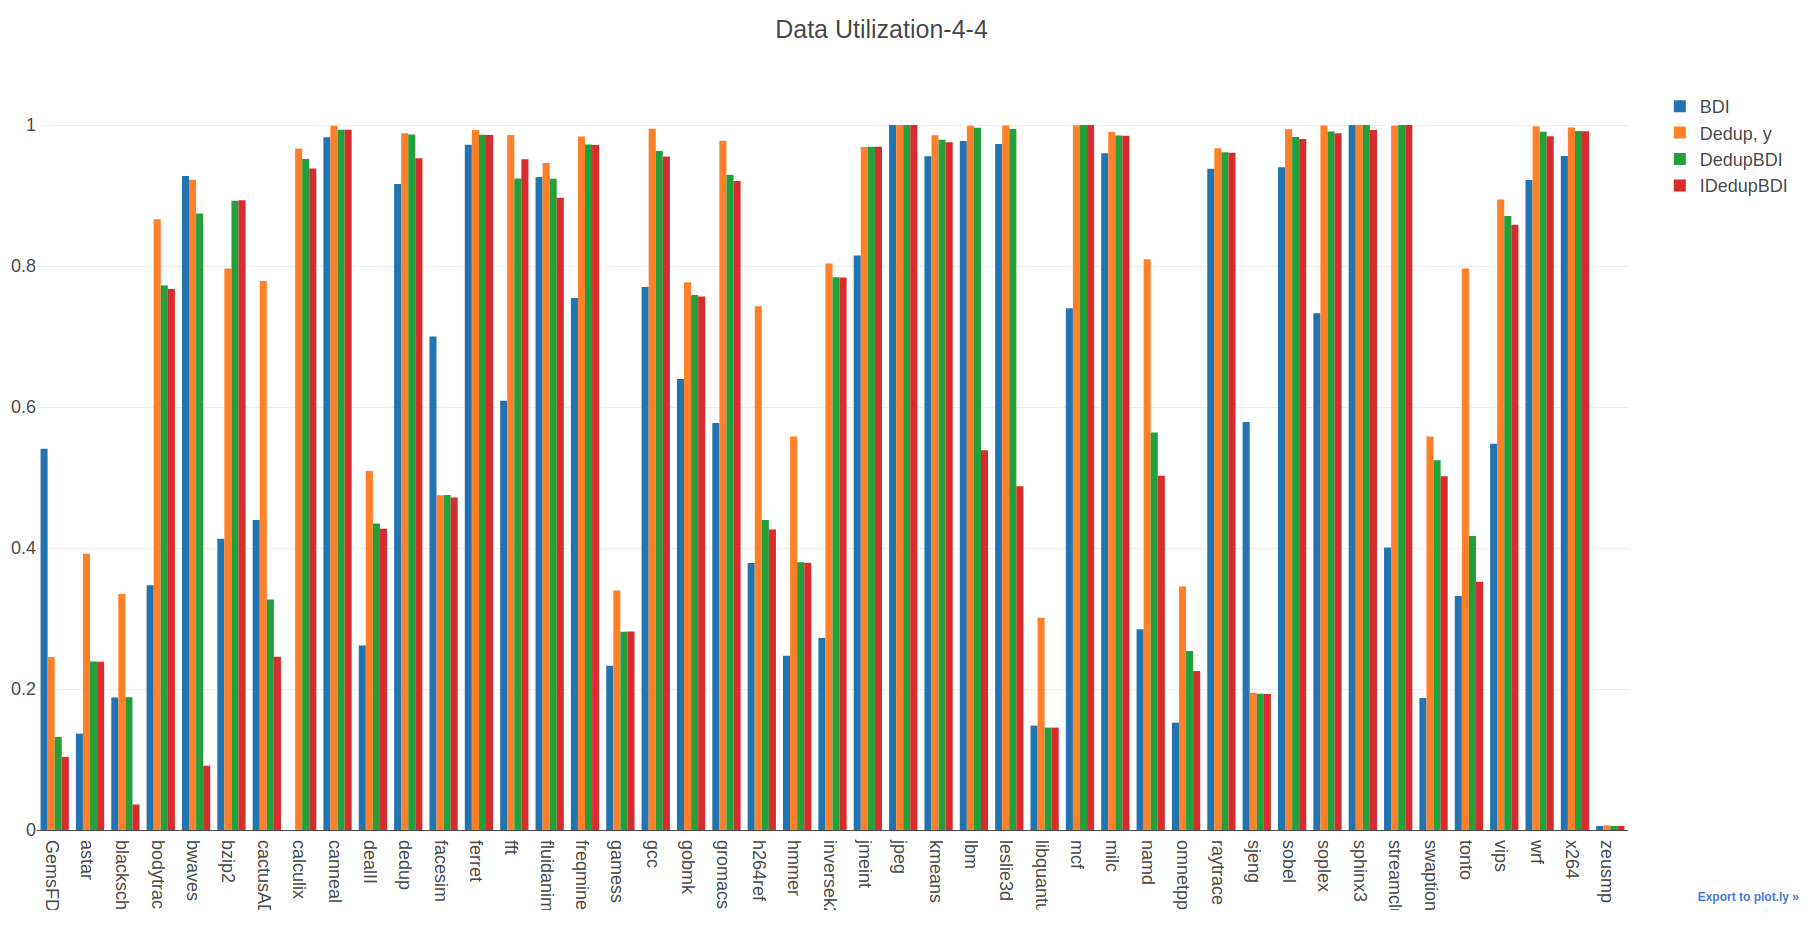
\includegraphics[width=\textwidth]{all-datautil.png}
    \end{subfigure}
    \caption[All benchmarks: Utilization]{Showing tag and data utilization ratio for all benchmarks using all types of compressed 4MB caches with tags four times data.}
    \label{fig:all_util}
\end{figure}
Results generated from other cache sizes (ranging from 0.5MB to 8MB) are very similar, we have chosen the 4MB-4 as a representative.

\section{Performance}
\label{sec:Performance}
\begin{table}[]
    \centering
    \small
    \setlength\tabcolsep{2pt}
    \begin{tabular}{|l|l|l|l|l|l|l|l|}
        \hline
        \textbf{Benchmark} & \textbf{Cache Sensitive}                                    & \textbf{Benchmark} & \textbf{Cache Sensitive}                                      & \textbf{Benchmark} & \textbf{Cache Sensitive}                                     & \textbf{Benchmark} & \textbf{Cache Sensitive}                                      \\ \hline
        fft                & \begin{tabular}[c]{@{}l@{}}Big Sizes \\ (Semi)\end{tabular} & fluidanimate       & None                                                          & gromacs            & \begin{tabular}[c]{@{}l@{}}Small Sizes \\ (Semi)\end{tabular} & wrf                & All                                                           \\ \hline
        inversek2j         & None                                                        & freqmine           & None                                                          & cactusADM          & \begin{tabular}[c]{@{}l@{}}All \\ (Semi)\end{tabular}         & bzip2              & All                                                           \\ \hline
        jmeint             & None                                                        & raytrace           & None                                                          & leslie3d           & \begin{tabular}[c]{@{}l@{}}Big Sizes \\ (Semi)\end{tabular}   & gcc                & All                                                           \\ \hline
        jpeg               & None                                                        & streamcluster      & None                                                          & namd               & None                                                          & mcf                &                                                               \\ \hline
        kmeans             & None                                                        & swaptions          & None                                                          & dealII             & Small Sizes                                                   & gobmk              & \begin{tabular}[c]{@{}l@{}}Small Sizes \\ (Semi)\end{tabular} \\ \hline
        sobel              & None                                                        & vips               & \begin{tabular}[c]{@{}l@{}}Small Sizes \\ (Semi)\end{tabular} & soplex             & \begin{tabular}[c]{@{}l@{}}All \\ (Semi)\end{tabular}         & hmmer              & \begin{tabular}[c]{@{}l@{}}Small Sizes \\ (Semi)\end{tabular} \\ \hline
        blackscholes       & None                                                        & x264               & None                                                          & calculix           & Small Sizes                                                   & sjeng              & None                                                          \\ \hline
        bodytrack          & None                                                        & bwaves             & None                                                          & GemsFDTD           &                                                               & libquantum         & Mid Sizes                                                     \\ \hline
        canneal            & \begin{tabular}[c]{@{}l@{}}All \\ (Semi)\end{tabular}       & gamess             & \begin{tabular}[c]{@{}l@{}}Small Sizes \\ (Semi)\end{tabular} & tonto              & \begin{tabular}[c]{@{}l@{}}Small Sizes \\ (Semi)\end{tabular} & h264ref            &                                                               \\ \hline
        dedup              & None                                                        & milc               &                                                               & lbm                & None                                                          & omnetpp            & Small Sizes                                                   \\ \hline
        facesim            & None                                                        & zeusmp             & None                                                          & sphinx3            & Big Sizes                                                     & astar              & All                                                           \\ \hline
        ferret             & \begin{tabular}[c]{@{}l@{}}All\\ (Semi)\end{tabular}        &                    &                                                               &                    &                                                               &                    &                                                               \\ \hline
        \end{tabular}
    \caption{All benchmarks and their cache behavior}
    \label{tab:cachesense}
\end{table}
\begin{figure}
    \begin{subfigure}{\textwidth}
        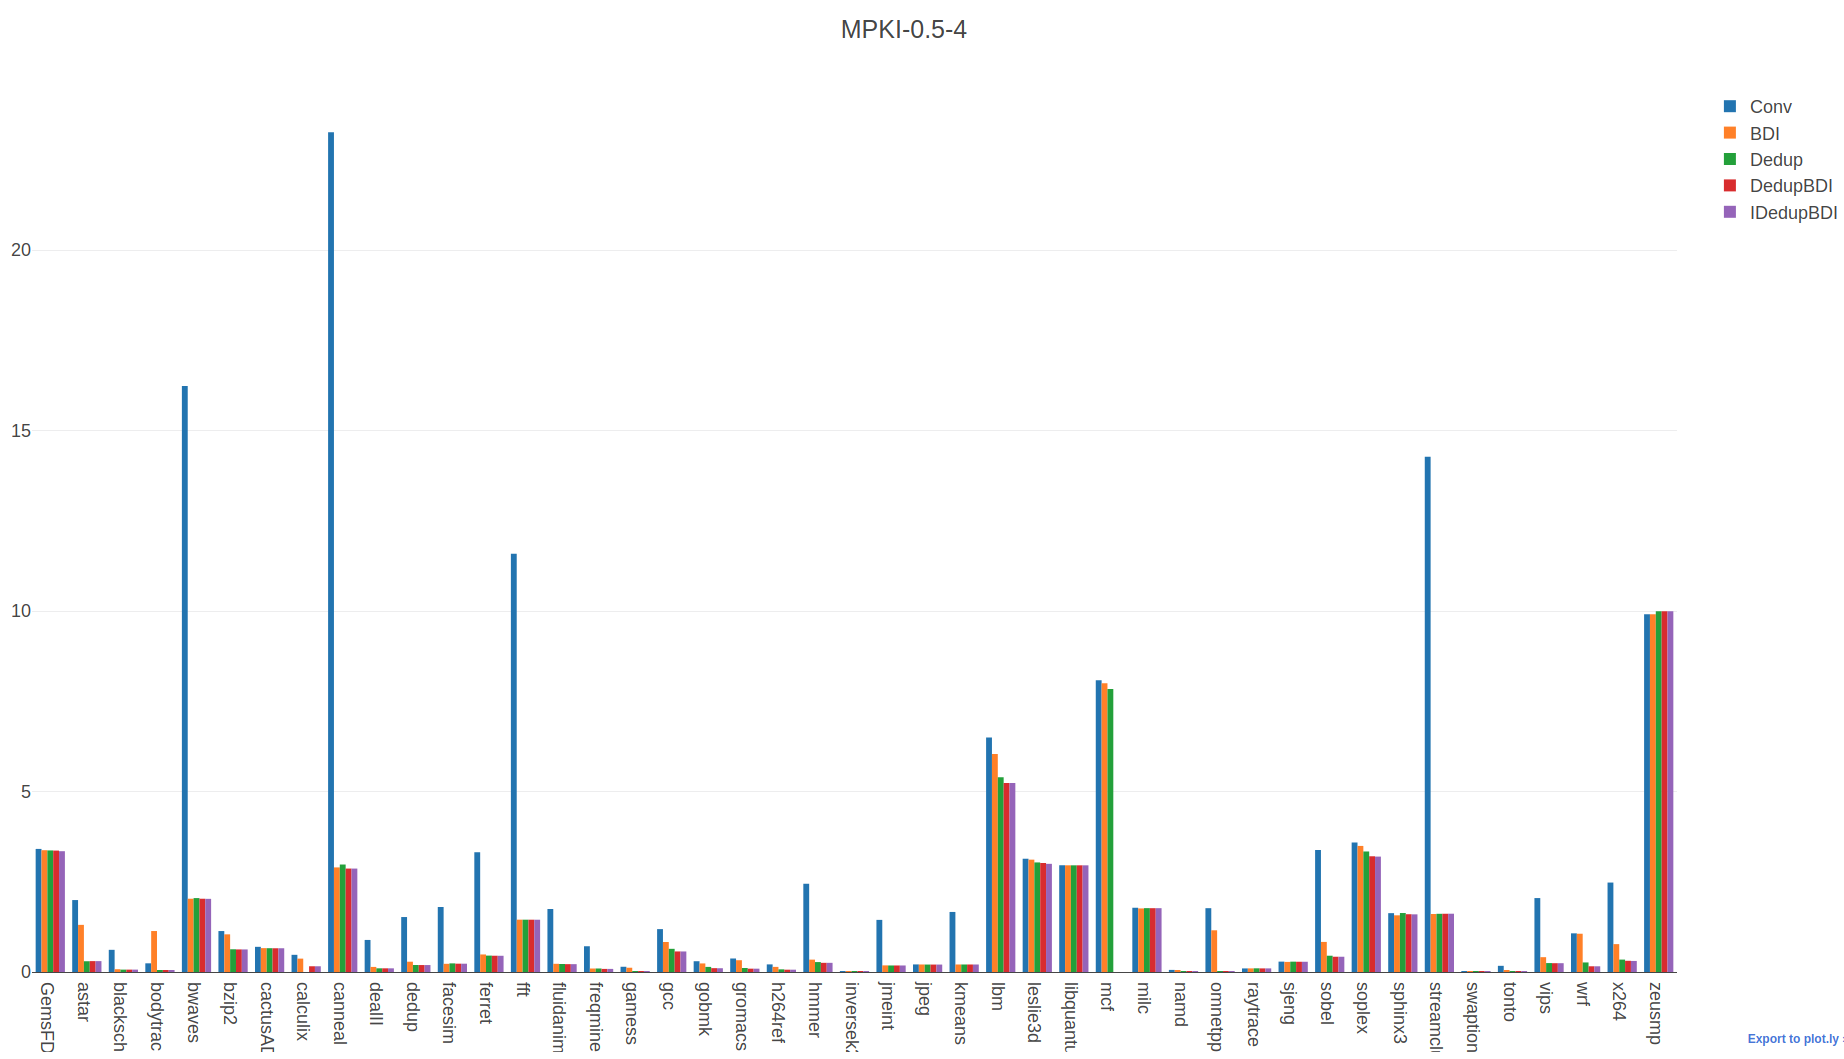
\includegraphics[width=\textwidth]{all05-mpki.png}
    \end{subfigure}
    \begin{subfigure}{\textwidth}
        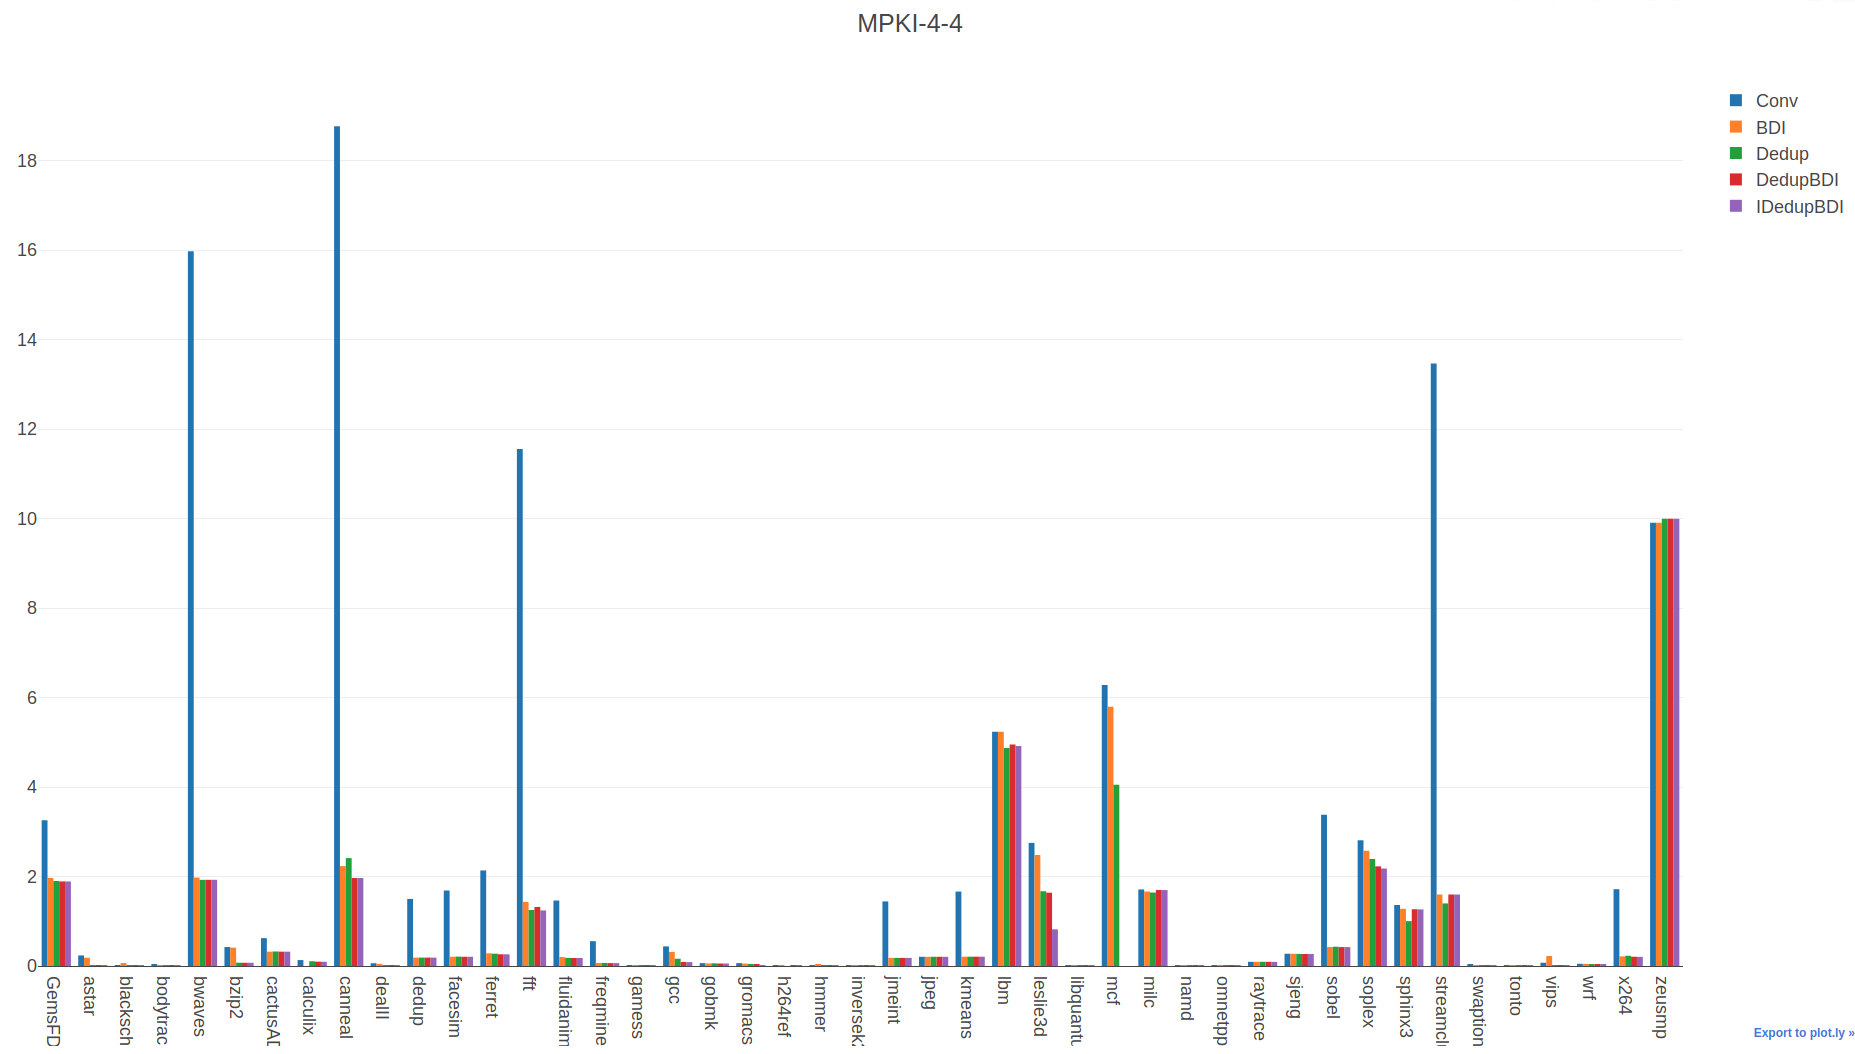
\includegraphics[width=\textwidth]{all4-mpki.png}
    \end{subfigure}
    \caption[All benchmarks: MPKI]{Showing LLC MPKI for conventional and all types of compressed 0.5 and 4MB caches with tags four times data.}
    \label{fig:all_mpki}
\end{figure}
\begin{figure}
    \begin{subfigure}{\textwidth}
        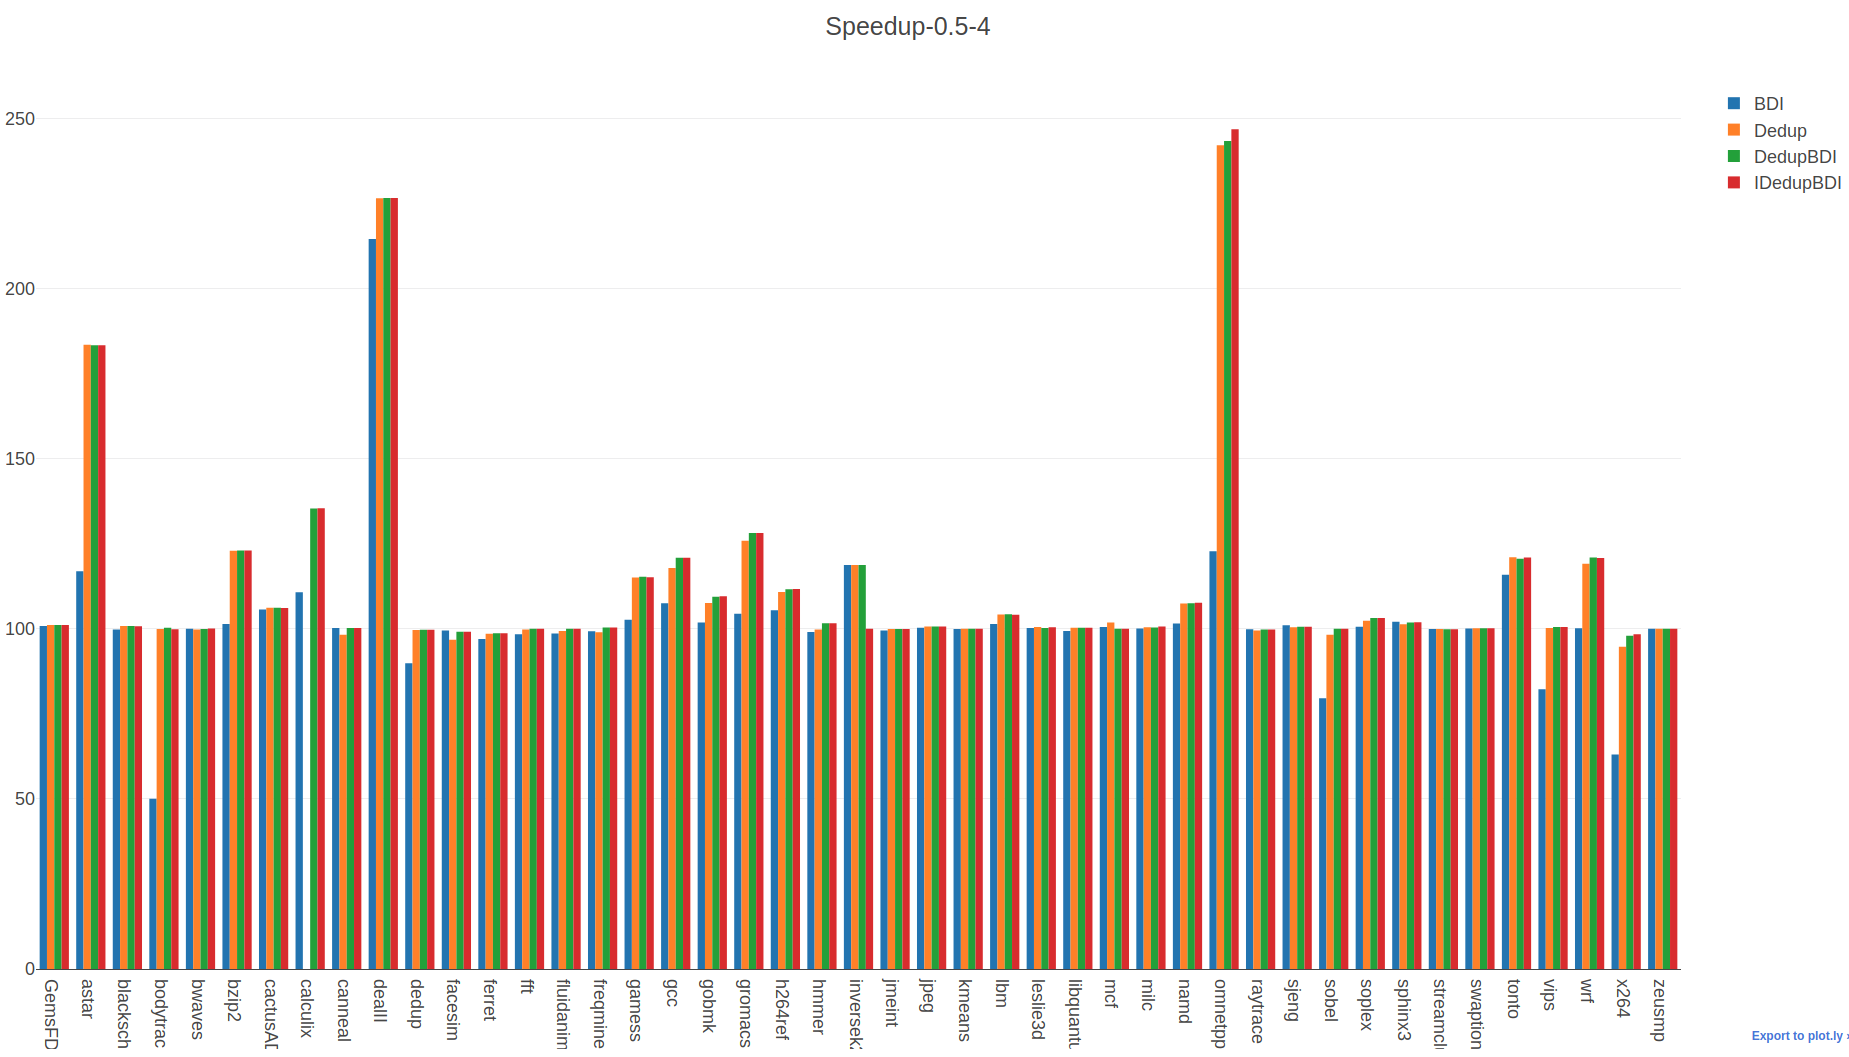
\includegraphics[width=\textwidth]{all05-speedup.png}
    \end{subfigure}
    \begin{subfigure}{\textwidth}
        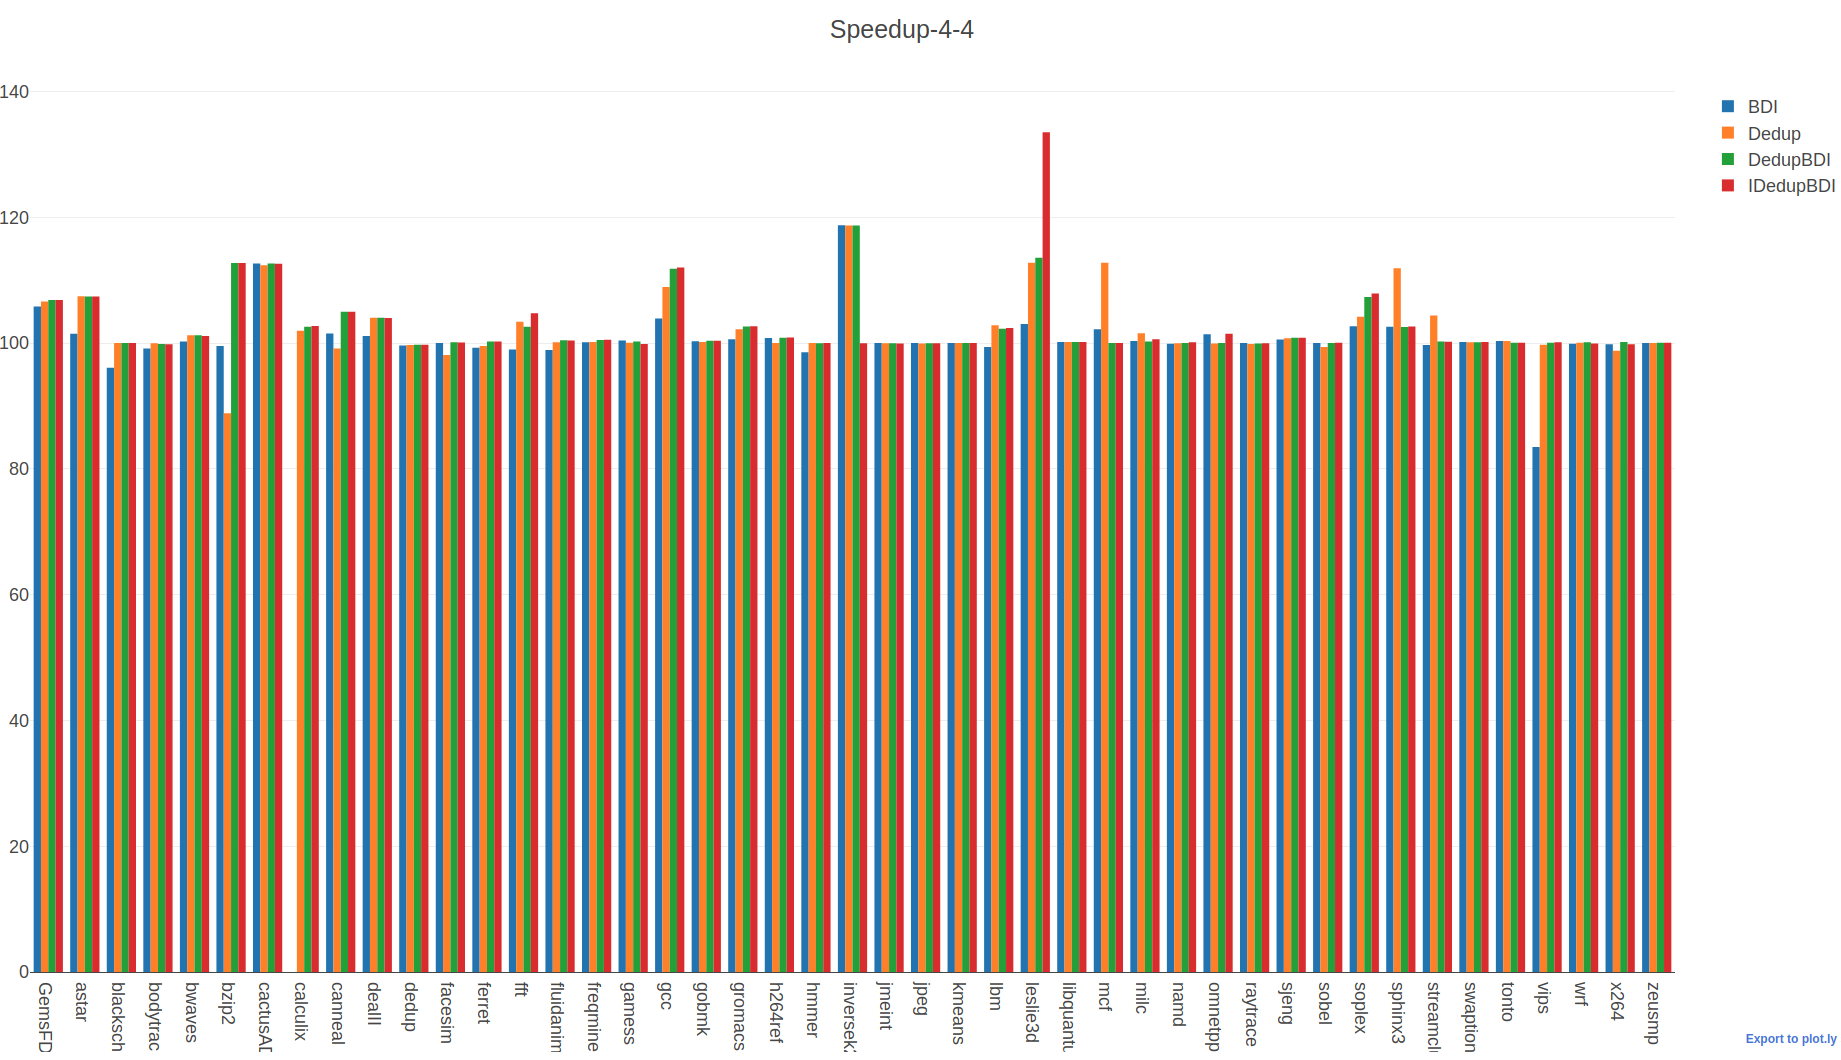
\includegraphics[width=\textwidth]{all4-speedup.png}
    \end{subfigure}
    \caption[All benchmarks: Speedup]{Showing Speedup for all types of compressed 0.5 and 4MB caches with tags four times data against conventional same size caches.}
    \label{fig:all_speedup}
\end{figure}
Figure \ref{fig:all_mpki} shows the MPKI for all the benchmarks when simulated with conventional and compressed 0.5MB and 4MB LLC caches with tags four times the data lines. It shows that compressed caches reduce MPKIs in LLC. DedupBDI is either the same as Dedup or BDI or is outperforming them.\par
However, the decrease of MPKI doesn't always necessitate speedup. The benchmark access patterns and cache sensitivity also play a role. Table \ref{tab:cachesense} shows the behavior of all benchmarks over a range fo cache sizes. Every benchmark is classified as cache sensitive, cache insensitive, or cache sensitive at a specific cache size range.
Figure \ref{fig:all_speedup} shows the speedup for all the benchmarks when simulated with a compressed 0.5MB and 4MB LLC caches with tags four times the data lines, respectively. We have chosen those two sizes because some benchmarks are only cache sensitive with lower cache sizes while others are only cache sensitive at higher cache sizes.\par
For the cache insensitive benchmarks, the DedupBDI cache performs as fast as the conventional caches. It does not provide anymore speedup. But it allows the data to be compressed, providing area and power savings. For the cache sensitive benchmarks, DedupBDI outperforms the conventional, Dedup, and DedupBDI caches altogether.

\section{Tag to Data Ratio}
\label{sec:tagratio}
\begin{figure}
    \begin{subfigure}{\textwidth}
        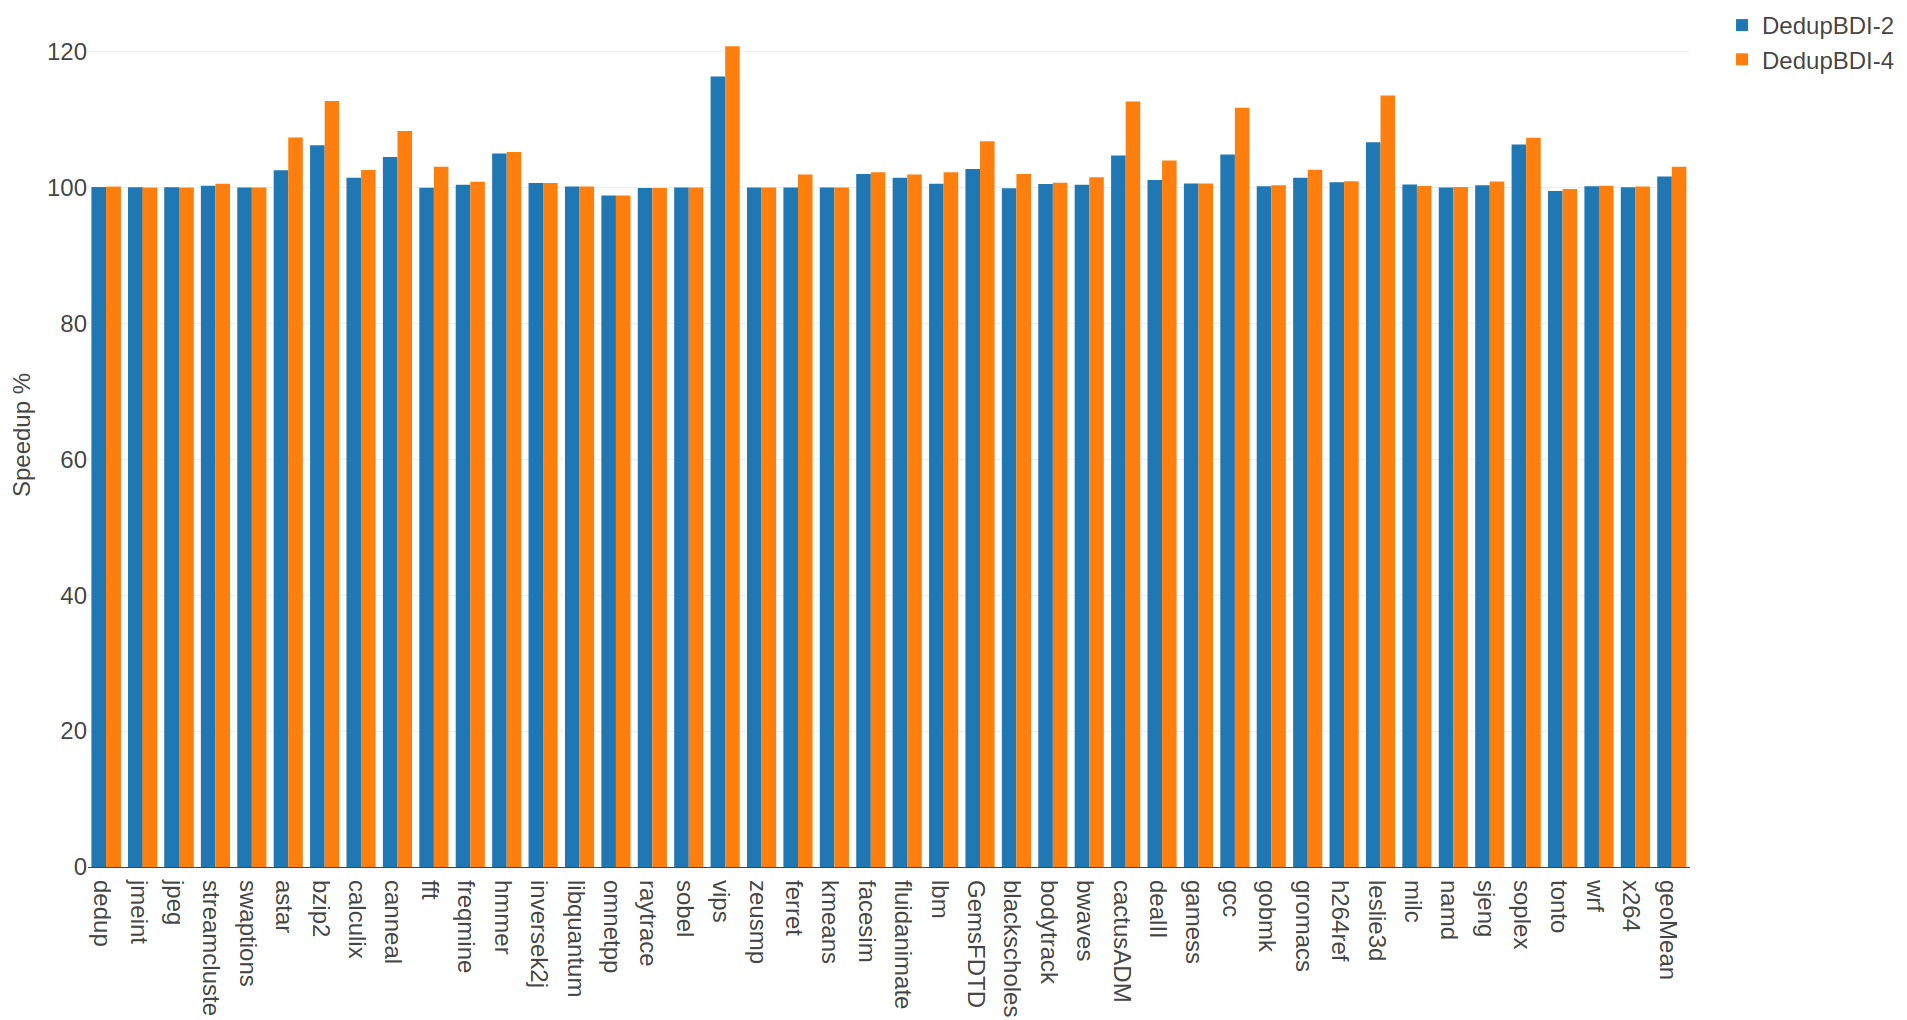
\includegraphics[width=\textwidth]{compare-speedup.png}
    \end{subfigure}
    \begin{subfigure}{\textwidth}
        \includegraphics[width=\textwidth]{compare-compression.png}
    \end{subfigure}
    \caption[All benchmarks: Tag Ratio]{Showing performance and compression ratio for all benchmarks using DedupBDI 4MB caches with tags four times data and twice the data.}
    \label{fig:all_compare}
\end{figure}
Figure \ref{fig:all_compare} shows the difference between two 4MB DedupBDI caches, one with tags twice the data entries and the other with tags four times the entries. Using the tags as four times the data entries means the data array will be twice as small but it also requires compression to be highly effective. Otherwise the cache will run out of data space quickly and throttle the performance. As Figure \ref{fig:all_compare} shows, the smaller 4MB-4 cache achieves better performance than the 4MB-2 and has better compression ratio. We've chosen caches with four times the tags to be our default compressed cache size.


\section{Overhead Analysis}
\label{sec:Overhead}
\begin{table}[]
    \centering
    \begin{tabular}{lllll}
               & Conv   & BDI    & Dedup  & DedupBDI \\ \hline
    Tags       &        &        &        &          \\
    \# Entries & 8192   & 8192   & 8192   & 8192     \\
    Entry Size & 49b    & 49b    & 49b    & 49b      \\
    Overhead   & 6b     & 15b    & 35b    & 42b      \\
    Total Size & 55KB   & 64KB   & 84KB   & 91KB     \\ \hline
    Data       &        &        &        &          \\
    \# Entries & 8192   & 2048   & 2048   & 2048     \\
    Entry Size & 64B    & 64B    & 64B    & 64B      \\
    Overhead   &        &        & 11b    & 11B      \\
    FreeList   &        &        & 2.75KB & 896B     \\
    Total Size & 0.5MB  & 125KB  & 133.5KB & 150.875KB   \\ \hline
    Hash       &        &        &        &          \\
    \# Entries &        &        & 64     & 64       \\
    Entry Size &        &        & 10b    & 10b      \\
    Overhead   &        &        & 11b    & 14b      \\
    Total Size &        &        & 168B   & 192B     \\ \hline
    Total Bank Size & 567KB & 189KB & 217.6KB & 242KB  
    \end{tabular}
    \caption{4MB cache size and overhead in all configurations.}
    \label{tab:overhead}
\end{table}
Table \ref{tab:overhead} shows the overheads in one bank in the cache designs we have, assuming an 8 banked cache, with an associativity of 16, cache size of 4MB and LRU replacement policy. The overhead in all caches comes from three (four) different sources:
\begin{itemize}
    \item \textbf{Tag Overhead:}
    \begin{itemize}
        \item \textbf{conventional:} In conventional caches, assuming LRU replacement policy, the tag overhead per entry consists of one bit for Valid, one for Dirty, and log2(associativity) bits for the LRU replacement. 
        \item \textbf{BDI:} In BDI there's an extra overhead of 4 bits for compression encoding and log2(associativity*\#SegmentsPerLine) bits for segment pointers. Along with the normal overhead from a conventional cache. Note that in BDI the data array has half or one quarter of the associativity of the tag array.
        \item \textbf{Dedup:} On top of the conventional cache overhead, Dedup adds two pointers per tag entry for the next/previous tag to build a linked list, each one of those is log2(\#Tags/associativity) bits. It also adds pointers to the data line associated with it. Since Dedup data arrays are direct mapped the data pointer size is log2(\#Data).
        \item \textbf{DedupBDI:} DedupBDI adds the same overhead as the BDI cache. It also adds the same linked list pointers from the Dedup cache, but it's data pointer size is different from the Dedup cache. Because the data array in DedupBDI maintains its associativity, the data pointer size is log2(\#Data/associativity).
    \end{itemize}
    \item \textbf{Data Overhead:}
    \begin{itemize}
        \item \textbf{conventional:} A conventional cache has no overheads in its data array.
        \item \textbf{BDI:} Similar to a conventional cache, A BDI cache does not have any metadata in its data array and thus does not have any overhead.
        \item \textbf{Dedup:} The data lines in a Dedup cache requires a pointer to the tag, which is enough to pint to the tag set so it has a size of log2(\#Tags/associativity). It also requires each data line to have a deduplication counter, which we described in \ref{ch:BackgroundMotiv} to be 2 bits.
        \item \textbf{DedupBDI:} The DedupBDI data array has the same overhead as its Dedup counterpart. Except the overhead is per segment instead of being per line. that means for each data line we have 8 Dedup data overheads.
    \end{itemize}
    \item \textbf{Extra Data Overhead:}
    \begin{itemize}
        \item \textbf{Dedup:} The Dedup cache maintains a free list of its free data lines. The free list is essentially a FIFO with the same number of entries as data lines, and with a width that's enough to hold a pointer to the corresponding data line (i.e. log2(\#Data)).
        \item \textbf{DedupBDI:} The DedupBDI cache maintains 8 different free lists. Each of them is a FIFO with the same number of sets as data sets (i.e. Data lines/associativity), with a width that's enough to hold a pointer to the set (i.e. log2(\#Data/associativity)).
    \end{itemize}
    \item \textbf{Hash Array:} The Dedup and DedupBDI have the same hash array design. The hash array saves part of the hash as a tag while the other part is used as an index. The hash array then has the size of \#Hash*(HashSize-log2(\#Hash/associativity)). The Dedup and DedupBDI hash arrays then have some extra overhead:
    \begin{itemize}
        \item \textbf{Dedup:} each hash entry has a data pointer of size log2(\#Data)
        \item \textbf{DedupBDI:} each hash entry has a data pointer of size log2(\#Data/associativity) and segment pointer of size log2(associativity*\#SegmentsPerLine) bits.
    \end{itemize}
\end{itemize}
It's obvious that DedupBDI has the highest amount of overhead. But it also gains the most savings and speedups.

\section{Area and Power}
\label{sec:areapower}
\begin{table}[]
    \centering
    \resizebox{\textwidth}{!}{%
    \begin{tabular}{llllll}
    \multicolumn{2}{c}{Cache}                                                 & \multicolumn{1}{c}{\begin{tabular}[c]{@{}c@{}}Access Latency\\ (ns)\end{tabular}} & \multicolumn{1}{c}{\begin{tabular}[c]{@{}c@{}}Dynamic Read\\ Energy (nJ)\end{tabular}} & \multicolumn{1}{c}{\begin{tabular}[c]{@{}c@{}}Leakage Power\\ (mW)\end{tabular}} & \multicolumn{1}{c}{Area (mm2)} \\ \hline
    \multicolumn{1}{l|}{\multirow{5}{*}{CONV}}     & \multicolumn{1}{l|}{0.5} & 1.040842                                                                          & .28134914                                                                              & 353.32648                                                                        & 12.2026068                     \\
    \multicolumn{1}{l|}{}                          & \multicolumn{1}{l|}{1}   & 1.116541                                                                          & .29846783                                                                              & 530.37712                                                                        & 13.073461                      \\
    \multicolumn{1}{l|}{}                          & \multicolumn{1}{l|}{2}   & 1.285388                                                                          & .33135866                                                                              & 884.79016                                                                        & 14.771159                      \\
    \multicolumn{1}{l|}{}                          & \multicolumn{1}{l|}{4}   & 1.46331                                                                           & .3967712                                                                               & 1579.6440                                                                        & 18.129441                      \\
    \multicolumn{1}{l|}{}                          & \multicolumn{1}{l|}{8}   & 1.917741                                                                          & .526493                                                                                & 2978.4016                                                                        & 24.880933                      \\ \cline{1-2}
    \multicolumn{1}{l|}{\multirow{5}{*}{BDI}}      & \multicolumn{1}{l|}{0.5} & 1.010391                                                                          & .26910215                                                                              & 236.31936                                                                        & 11.605206                      \\
    \multicolumn{1}{l|}{}                          & \multicolumn{1}{l|}{1}   & 1.045793                                                                          & .27524057                                                                              & 298.75176                                                                        & 11.921437                      \\
    \multicolumn{1}{l|}{}                          & \multicolumn{1}{l|}{2}   & 1.126943                                                                          & .28691374                                                                              & 415.8200                                                                         & 12.527563                      \\
    \multicolumn{1}{l|}{}                          & \multicolumn{1}{l|}{4}   & 1.297986                                                                          & .3083546                                                                               & 655.4520                                                                         & 13.701536                      \\
    \multicolumn{1}{l|}{}                          & \multicolumn{1}{l|}{8}   & 1.385186                                                                          & .3511512                                                                               & 1130.4840                                                                        & 15.981861                      \\ \cline{1-2}
    \multicolumn{1}{l|}{\multirow{5}{*}{DEDUP}}    & \multicolumn{1}{l|}{0.5} & 1.026490                                                                          & .26946535                                                                              & 240.20488                                                                        & 11.623081                      \\
    \multicolumn{1}{l|}{}                          & \multicolumn{1}{l|}{1}   & 1.070838                                                                          & .27615777                                                                              & 310.98856                                                                        & 11.976806                      \\
    \multicolumn{1}{l|}{}                          & \multicolumn{1}{l|}{2}   & 1.156487                                                                          & .28876076                                                                              & 440.1304                                                                         & 12.642104                      \\
    \multicolumn{1}{l|}{}                          & \multicolumn{1}{l|}{4}   & 1.396239                                                                          & .3130041                                                                               & 714.2168                                                                         & 13.976212                      \\
    \multicolumn{1}{l|}{}                          & \multicolumn{1}{l|}{8}   & 1.481563                                                                          & .3610318                                                                               & 1263.6328                                                                        & 16.601801                      \\ \cline{1-2}
    \multicolumn{1}{c|}{\multirow{5}{*}{DEDUPBDI}} & \multicolumn{1}{l|}{0.5} & .971216                                                                           & .27016215                                                                              & 246.69448                                                                        & 11.655013                      \\
    \multicolumn{1}{c|}{}                          & \multicolumn{1}{l|}{1}   & 1.085028                                                                          & .27733513                                                                              & 324.34256                                                                        & 12.039511                      \\
    \multicolumn{1}{c|}{}                          & \multicolumn{1}{l|}{2}   & 1.172562                                                                          & .29132959                                                                              & 468.7792                                                                         & 12.778273                      \\
    \multicolumn{1}{c|}{}                          & \multicolumn{1}{l|}{4}   & 1.428335                                                                          & .3183339                                                                               & 773.8560                                                                         & 14.257854                      \\
    \multicolumn{1}{c|}{}                          & \multicolumn{1}{l|}{8}   & 1.522417                                                                          & .3725894                                                                               & 1392.7656                                                                        & 17.212904                      \\ \cline{1-2}
    \end{tabular}%
    }
    \caption{Area, Power, Energy, and Access Latency for all cache sizes and configurations.}
    \label{tab:areapower}
\end{table}
We used cacti6\cite{cacti} to get power and area estimations for all the cache types and sizes we simulated. The results are shown in \ref{tab:areapower}. The results in the table are consistent with what we've discussed so far. Compressed caches have lower access latencies, energy and power consumption than their conventional counterparts because of their lesser size. With DedupBDI consuming the most resources out of the compressed caches. The extra resources however are justified as they allow better speedup and compression.
%% The following is a directive for TeXShop to indicate the main file
%%!TEX root = diss.tex

\chapter{Related Work}
\label{ch:Related Work}
In this section we describe some of the previous work in cache compression. We discuss how they are different that our picked algorithms.
\section{Special Case Schemes}
\subsection{Zero Content Augmented Cache}
The Zero Content Augmented~\cite{zca} cache takes advantage of the fact that zero lines are very common in today's benchmarks. It uses a special structure called zero content cache to complement normal caches. This zero content cache only saves tags for data lines that are completely null. Special care has to taken to handle cases where a line changes and thus has to be moved from one of the caches to the other one. The choice to use an external zero content cache simplifies the design process. It allows seamless integration with any normal cache without changing its underlying structure.

\section{Data Compression}
\subsection{Frequent Pattern Compression}
\label{ssec:FPC}
Frequent Pattern Compression~\cite{fpc} is one of the earliest cache compression techniques proposed. It is focused on compressing data on an intra-line granularity. If is based on the observation that some patterns are more frequent in data and can be represented by fewer bits. It takes advantage of this observation by dividing each cache line to words. Each word is represented as a 3-bit encoding prefix then a (un)compressed data form. The patterns are frequent enough to achieve good compression, but in the worst case scenario an uncompressed data work will be represented in 35 bits instead of 32. The FPC cache uses tag and data array decoupling, similar to Dedup, to allow more tags than data lines. This simple scheme provides good compression ratios and is not complex to implement.
\subsection{SC2}
The SC2 cache~\cite{sc2} is a statistical compression caches. It uses Huffman-coding~\cite{huffman1952method} to assign variable length codes to data based on their probability of occurance. This allows saving small codes for values with high probability of occurance like zeros for example. While this cache achieves good compression ratios, its downside is that it requires a sampling phase to collect statistics on the frequency of values, and requires an extra structure for recording the frequency of values, it also requires software routines to do encoding after sampling.
\subsection{HyComp}
The HyComp cache compression~\cite{hycomp} is a hybrid cache compression algorithm. It selects different cache compression algorithm depending on the data type. It first employs a predictor to predict the data type in each line. Then it tries to use the appropriate cache compression for this data type. It uses SC2 for integer compression, BDI for pointer compression, ZCA for zero lines, and it also introduces a new compression technique called FP-H for floating points. The combination of those different algorithms and using them with different data types allows this cache to achieve high compression ratios. However, It also increases the complexity and overhead. Because of this, we chose to only implement BDI as intra-line compression, although our implementation should be extendable to support any intra-line compression. It will only require changing the compression/decompression hardware, and the compression metadata in the cache arrays.

\section{Dictionary Based Compression}
\subsection{CPACK}
CPACK is a combination of dictionary compression and frequent pattern compression (not to be mistaken with the~\ref{ssec:FPC}). It uses encoding for frequently observed patterns and combines this with using dictionaries or partial dictionaries for frequently encountered data values. It maintains dictionaries per data line and is able to compress multiple words in parallel at the same time.
\subsection{Dictionary Sharing}
The Dictionary Sharing cache (DISH) is a dictionary based compression cache. The authors make the observation that there is sufficient value locality in consecutive data lines to merit using dictionaries on a scale bigger than one data line. They use dictionaries on a granularity from one cache line to a super-block (four cache lines). Like other compressed caches it also increases tags over data entries, but it does so using one single tag for a whole super-block.

% \section{Software Compression}


%    3. Notes
%    4. Footnotes

%    5. Bibliography
\begin{singlespace}
\raggedright
\bibliographystyle{abbrvnat}
\bibliography{biblio}
\end{singlespace}

\appendix
%    6. Appendices (including copies of all required UBC Research
%       Ethics Board's Certificates of Approval)
%\include{reb-coa}	% pdfpages is useful here
\chapter{Supporting Materials}

This would be any supporting material not central to the dissertation.
For example:
\begin{itemize}
\item additional details of methodology and/or data;
\item diagrams of specialized equipment developed.;
\item copies of questionnaires and survey instruments.
\end{itemize}


\backmatter
%    7. Index
% See the makeindex package: the following page provides a quick overview
% <http://www.image.ufl.edu/help/latex/latex_indexes.shtml>


\end{document}
